%===========================================================
% This is the thesis template for the Statistics major at
% Amherst College. Brittney E. Bailey (bebailey@amherst.edu)
% adapted this template from the Reed College LaTeX thesis
% template in January 2019 with major updates in April 2020.
% Please send any comments/suggestions: bebailey@amherst.edu

% Most of the work for the original document class was done
% by Sam Noble (SN), as well as this template. Later comments
% etc. by Ben Salzberg (BTS). Additional restructuring and
% APA support by Jess Youngberg (JY). Email: cus@reed.edu
%===========================================================

\documentclass[12pt, twoside]{amherstthesis}
\usepackage{graphicx,latexsym}
\usepackage{amsmath}
\usepackage{amssymb,amsthm}
\usepackage{longtable,booktabs} %setspace loaded in .cls
\usepackage[hyphens]{url}
\usepackage{hyperref}
\usepackage{lmodern}
\usepackage{float}
\floatplacement{figure}{H}
\usepackage{rotating}
\usepackage{fancyvrb}
% User-added packages:
	\usepackage{booktabs}
 \usepackage{longtable}
 \usepackage{array}
 \usepackage{multirow}
 \usepackage{wrapfig}
 \usepackage{float}
 \usepackage{colortbl}
 \usepackage{pdflscape}
 \usepackage{tabu}
 \usepackage{threeparttable}
 \usepackage{threeparttablex}
 \usepackage[normalem]{ulem}
 \usepackage{makecell}
 \usepackage{xcolor}
% End user-added packages

%===========================================================
% BIBLIOGRAPHY FORMATTING

% Next line commented out by CII
%%% \usepackage{natbib}
% Comment out the natbib line above and uncomment the
% following two lines to use the new biblatex-chicago style,
% for Chicago A. Also make some changes at the end where the
% bibliography is included.
%\usepackage{biblatex-chicago}
%\bibliography{thesis}


%===========================================================
% HYPERLINK FORMATTING

% Added by CII (Thanks, Hadley!)
% Use ref for internal links
\renewcommand{\hyperref}[2][???]{\autoref{#1}}
\def\chapterautorefname{Chapter}
\def\sectionautorefname{Section}
\def\subsectionautorefname{Subsection}
% End of CII addition
\usepackage{xcolor}
\hypersetup{
    colorlinks,
    linkcolor={red!50!black},
    citecolor={blue!50!black},
    urlcolor={blue!80!black}
}

%===========================================================
% CAPTION FORMATTING

% Added by CII
\usepackage{caption}
\captionsetup{width=5in}
% End of CII addition

%===========================================================
% TITLE FORMATTING

\renewcommand{\contentsname}{Table of Contents}

\usepackage{titlesec}
%%%%%%%%
% How to use titlesec:
% \titleformat{⟨command⟩}[⟨shape⟩]{⟨format⟩}{⟨label⟩}{⟨sep⟩}
%  {⟨before-code⟩}[⟨after-code⟩]
%%%%%%%%

\titleformat{\chapter}[hang]
{\normalfont%
    \Large% %change this size to your needs for the first line
    \bfseries}{\chaptertitlename\ \thechapter}{1em}{%
      %change this size to your needs for the second line
    }[]

\titleformat{\section}[hang]
{\normalfont%
    \large % %change this size to your needs for the first line
    \bfseries}{\thesection}{1em}{%
     %change this size to your needs for the second line
    }[]

\titleformat{\subsection}[hang]
{\normalfont%
    \normalsize % %change this size to your needs for the first line
    \bfseries}{\thesubsection}{1em}{%
     %change this size to your needs for the second line
    }[]

% \titleformat{\section}[display]
% {\normalfont%
%     \large% %change this size to your needs for the first line
%     \bfseries}{\chaptertitlename\ \thechapter}{20pt}{%
%     \normalsize %change this size to your needs for the second line
%     }


%===========================================================
% DOCUMENT FONT

% \usepackage{times}
% other fonts available eg: times, bookman, charter, palatino


%===========================================================
% PASSING FORMATS FROM RMD --> LATEX

%%%%%%%%
% NOTE: Dollar signs pass parameters between YAML inputs
% in index.Rmd and LaTeX
%%%%%%%%

\Abstract{
The abstract should be a short summary of your thesis work. A paragraph is usually sufficient here.

Missing data is ubiquitious in statistics: from nonresponse in survey studies to issues with data collection in field studies, it is
often unavoidable to encounter missing data in practice. Our thesis begins with an overview of missingness, specifically with
left-censored data, and introduces four different methods: substitution, maxmimum likelihood, kaplan-meier, and regression on order
statistics to combat this. We explore a simulation study to compare and contrast the effectiveness of these methods when considering
for the distribution of the data, censoring rates, and the size of the dataset in order to validate several claims made in several
papers regarding these methods. Finally, we explore left-censored data in the form of coal ash contamination in groundwater wells,
and apply our findings to this case study. Our results from our simulation study show that BLAH.
}

\Acknowledgments{
Use this space to thank those who have helped you in the thesis process (professors, staff, friends, family, etc.). If you had special funding to conduct your thesis work, that should be acknowledged here as well.
}

\Dedication{

}

\Preface{

}

% Formatting R code display
% Syntax highlighting #22
  \usepackage{color}
  \usepackage{fancyvrb}
  \newcommand{\VerbBar}{|}
  \newcommand{\VERB}{\Verb[commandchars=\\\{\}]}
  \DefineVerbatimEnvironment{Highlighting}{Verbatim}{commandchars=\\\{\}}
  % Add ',fontsize=\small' for more characters per line
  \usepackage{framed}
  \definecolor{shadecolor}{RGB}{248,248,248}
  \newenvironment{Shaded}{\begin{snugshade}}{\end{snugshade}}
  \newcommand{\AlertTok}[1]{\textcolor[rgb]{0.94,0.16,0.16}{#1}}
  \newcommand{\AnnotationTok}[1]{\textcolor[rgb]{0.56,0.35,0.01}{\textbf{\textit{#1}}}}
  \newcommand{\AttributeTok}[1]{\textcolor[rgb]{0.77,0.63,0.00}{#1}}
  \newcommand{\BaseNTok}[1]{\textcolor[rgb]{0.00,0.00,0.81}{#1}}
  \newcommand{\BuiltInTok}[1]{#1}
  \newcommand{\CharTok}[1]{\textcolor[rgb]{0.31,0.60,0.02}{#1}}
  \newcommand{\CommentTok}[1]{\textcolor[rgb]{0.56,0.35,0.01}{\textit{#1}}}
  \newcommand{\CommentVarTok}[1]{\textcolor[rgb]{0.56,0.35,0.01}{\textbf{\textit{#1}}}}
  \newcommand{\ConstantTok}[1]{\textcolor[rgb]{0.00,0.00,0.00}{#1}}
  \newcommand{\ControlFlowTok}[1]{\textcolor[rgb]{0.13,0.29,0.53}{\textbf{#1}}}
  \newcommand{\DataTypeTok}[1]{\textcolor[rgb]{0.13,0.29,0.53}{#1}}
  \newcommand{\DecValTok}[1]{\textcolor[rgb]{0.00,0.00,0.81}{#1}}
  \newcommand{\DocumentationTok}[1]{\textcolor[rgb]{0.56,0.35,0.01}{\textbf{\textit{#1}}}}
  \newcommand{\ErrorTok}[1]{\textcolor[rgb]{0.64,0.00,0.00}{\textbf{#1}}}
  \newcommand{\ExtensionTok}[1]{#1}
  \newcommand{\FloatTok}[1]{\textcolor[rgb]{0.00,0.00,0.81}{#1}}
  \newcommand{\FunctionTok}[1]{\textcolor[rgb]{0.00,0.00,0.00}{#1}}
  \newcommand{\ImportTok}[1]{#1}
  \newcommand{\InformationTok}[1]{\textcolor[rgb]{0.56,0.35,0.01}{\textbf{\textit{#1}}}}
  \newcommand{\KeywordTok}[1]{\textcolor[rgb]{0.13,0.29,0.53}{\textbf{#1}}}
  \newcommand{\NormalTok}[1]{#1}
  \newcommand{\OperatorTok}[1]{\textcolor[rgb]{0.81,0.36,0.00}{\textbf{#1}}}
  \newcommand{\OtherTok}[1]{\textcolor[rgb]{0.56,0.35,0.01}{#1}}
  \newcommand{\PreprocessorTok}[1]{\textcolor[rgb]{0.56,0.35,0.01}{\textit{#1}}}
  \newcommand{\RegionMarkerTok}[1]{#1}
  \newcommand{\SpecialCharTok}[1]{\textcolor[rgb]{0.00,0.00,0.00}{#1}}
  \newcommand{\SpecialStringTok}[1]{\textcolor[rgb]{0.31,0.60,0.02}{#1}}
  \newcommand{\StringTok}[1]{\textcolor[rgb]{0.31,0.60,0.02}{#1}}
  \newcommand{\VariableTok}[1]{\textcolor[rgb]{0.00,0.00,0.00}{#1}}
  \newcommand{\VerbatimStringTok}[1]{\textcolor[rgb]{0.31,0.60,0.02}{#1}}
  \newcommand{\WarningTok}[1]{\textcolor[rgb]{0.56,0.35,0.01}{\textbf{\textit{#1}}}}

% Formatting R code: set baselinestretch = 1.5 for double-spacing
\DefineVerbatimEnvironment{Highlighting}{Verbatim}{
  baselinestretch = 1,
  commandchars=\\\{\}}

% Formatting R output display: set baselinestretch = 1.5 for double-spacing
\DefineVerbatimEnvironment{verbatim}{Verbatim}{
  baselinestretch = 1,
  % indent from left margin
  xleftmargin = 1mm,
  % vertical grey bar on left side of R output
  frame = leftline,
  framesep = 0pt,
  framerule = 1.5mm, rulecolor = \color{black!15}
  }

\title{Parameter Estimation Methods with Left-Censored Missingness}
\author{Tony Ni}
\date{April 28, 2021}
\division{}
\advisor{Brittney Bailey}
% for second advisor
\institution{Amherst College}
\degree{Bachelor of Arts}
\department{Mathematics and Statistics}

% Fix from pandoc about cslreferences?
% https://github.com/mpark/wg21/issues/54
\newlength{\cslhangindent}
\setlength{\cslhangindent}{1.5em}
\newenvironment{CSLReferences}%
  {}%
  {\par}

% Added by CII
%%% Copied from knitr
%% maxwidth is the original width if it's less than linewidth
%% otherwise use linewidth (to make sure the graphics do not exceed the margin)
\makeatletter
\def\maxwidth{ %
  \ifdim\Gin@nat@width>\linewidth
    \linewidth
  \else
    \Gin@nat@width
  \fi
}
\makeatother

% ===========================================
% DOCUMENT SPACING

\setlength{\parskip}{0pt}
% Added by CII

\providecommand{\tightlist}{%
  \setlength{\itemsep}{0pt}\setlength{\parskip}{0pt}}


% ===========================================
% ===========================================
% ===========================================
\begin{document}

\doublespace
% Everything below added by CII
  \maketitle

\frontmatter % this stuff will be roman-numbered
\pagenumbering{roman}
\pagestyle{fancyplain}
%\pagestyle{fancy} % this removes page numbers from the frontmatter

  \begin{abstract}
    The abstract should be a short summary of your thesis work. A paragraph is usually sufficient here.

    Missing data is ubiquitious in statistics: from nonresponse in survey studies to issues with data collection in field studies, it is
    often unavoidable to encounter missing data in practice. Our thesis begins with an overview of missingness, specifically with
    left-censored data, and introduces four different methods: substitution, maxmimum likelihood, kaplan-meier, and regression on order
    statistics to combat this. We explore a simulation study to compare and contrast the effectiveness of these methods when considering
    for the distribution of the data, censoring rates, and the size of the dataset in order to validate several claims made in several
    papers regarding these methods. Finally, we explore left-censored data in the form of coal ash contamination in groundwater wells,
    and apply our findings to this case study. Our results from our simulation study show that BLAH.
  \end{abstract}
  \begin{acknowledgments}
    Use this space to thank those who have helped you in the thesis process (professors, staff, friends, family, etc.). If you had special funding to conduct your thesis work, that should be acknowledged here as well.
  \end{acknowledgments}

  \hypersetup{linkcolor=black}
  \setcounter{tocdepth}{2}
  \tableofcontents

  \addcontentsline{toc}{chapter}{List of Tables}\listoftables

  \addcontentsline{toc}{chapter}{List of Figures}\listoffigures


\mainmatter % here the regular arabic numbering starts
\pagenumbering{arabic}
\pagestyle{fancyplain} % turns page numbering back on

\hypertarget{intro}{%
\chapter{Introduction}\label{intro}}

The concept of missing data is ubiquitous across academic disciplines and often complicates real-world studies. Most studies utilize data collected through surveys, questionnaires, and/or field research which is why missing data is often unavoidable. Missing data can hinder one's ability to work with and analyze the phenomena at hand, giving rise to inaccurate or even misleading analyses.

Barnard \& Meng (1999) outline several significant issues when conducting analysis on missing data. Firstly, missing data can introduce bias in regards to parameter estimation. It can also lead to a reduction in statistical power, which can affect the conclusions one makes during studies involving hypothesis testing. Finally, missing data can introduce complications with statistical software and lead to functions not working as intended, if they have not accounted for the possibility of the data containing missingness.

This thesis will go into a more specific instance of missing data known as censoring, which is \emph{the condition when one has only partial information regarding the values of a measurement within a dataset}. In this chapter, we will introduce and define the three types of censored data, discuss the challenges with the reporting of censored data, and explore common statistical approaches to handling censored data.

\hypertarget{censored_data}{%
\section{Censored Data}\label{censored_data}}

As discussed previously, censored data is a specific type of missingness where one has only partial information regarding the values of a measurement in a dataset. There are three types of censoring which can occur: right censoring, interval censoring, and left censoring.

\hypertarget{right}{%
\subsection{Right Censoring}\label{right}}

Right censoring is a specific instance in which we only know that the true value of a data point lies above a certain threshold, but it is unknown by how much. Suppose a study on income and mortality is conducted with the variable of interest, \(T\), being the time measured from the start of the study to the death of the participant. The study has a duration of 5 years, in which participants are expected to submit a form regarding their annual income. The value for the participant would be considered to be right-censored if at any point during the study, they failed to follow-up, or if the participant was still alive at the conclusion of the 5 year study. In this design study, several possibilities can occur, illustrated in Figure \ref{fig:rightcensoringexample}.
\begin{figure}

{\centering 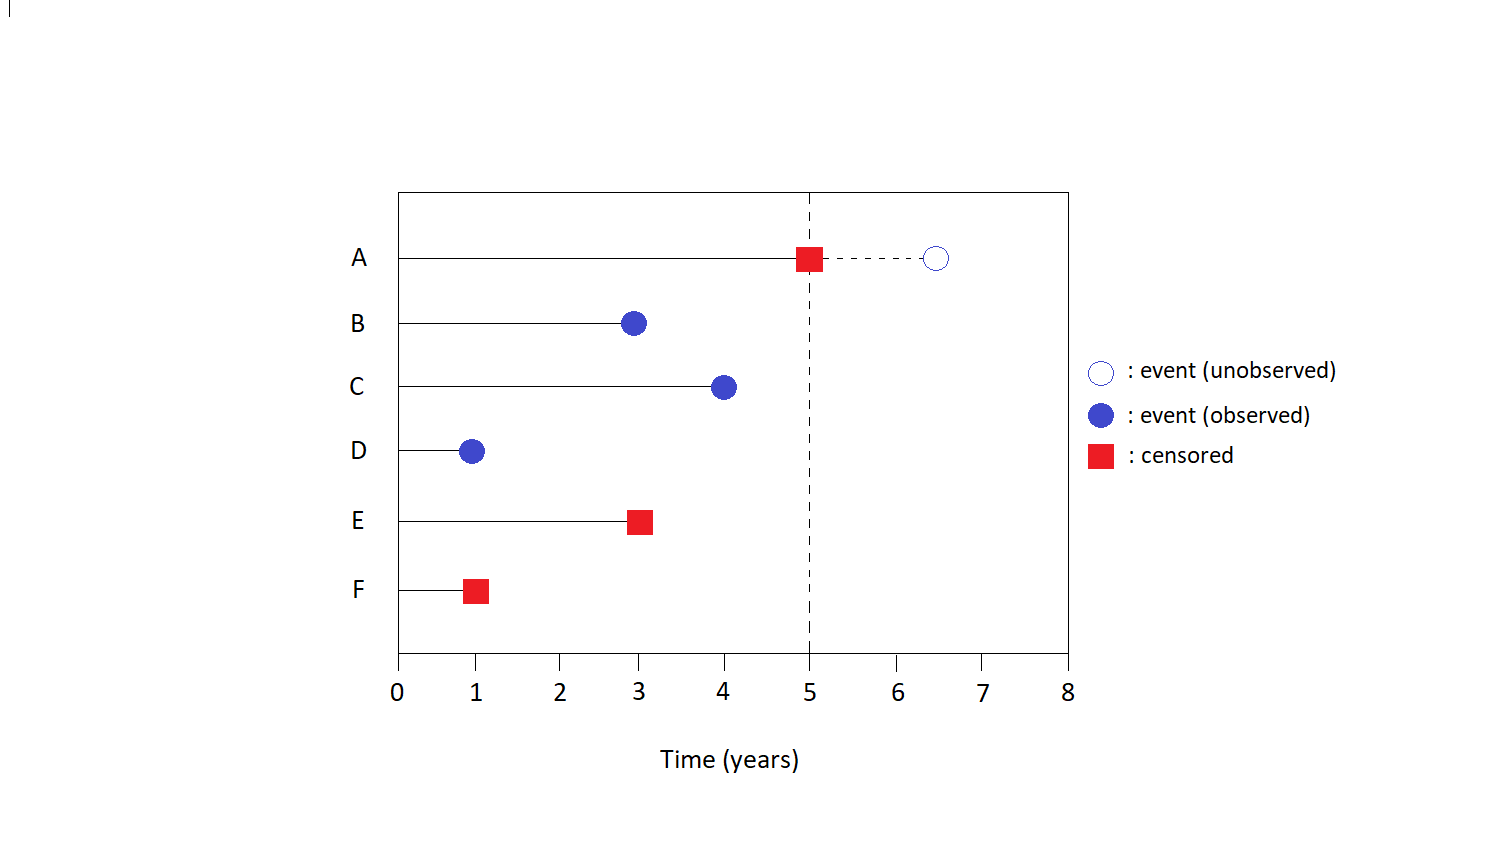
\includegraphics[width=1\linewidth]{figures/right_censoring_example} 

}

\caption{Right Censoring Example}\label{fig:rightcensoringexample}
\end{figure}
As illustrated by individual A in Figure \ref{fig:rightcensoringexample}, this individual lives on until the termination of the study. We don't know at what point they passed away exactly, since they didn't pass away during the time constraints of the study. As such, the only information we have is \(T > 5\).

If an individual does pass away at some point, \(t_i\), \emph{during} the study, then \(T = t_i\). This can be illustrated within Figure \ref{fig:rightcensoringexample} by individuals B, C, and D for which \(T = 3\), \(T = 4\), and \(T = 1\).

There is a final possibility for individuals who choose to censor themselves. Illustrated in Figure \ref{fig:rightcensoringexample} by individuals E and F, we can see that they are marked as censored at \(T = 3\) and \(T = 1\), respectively. These individuals may have chosen to stop submitting information to the study or drop out of the study entirely without warning. As we have no information about whether or not if they died or simply did not submit their form, all we know is that the individual died/will die at some point after the point at which they were censored.

Right censoring is the most common type of censoring and can often be found in clinical trial studies, mortality studies, and other forms of surival analyses.

\hypertarget{left}{%
\subsection{Left Censoring}\label{left}}
\begin{figure}

{\centering 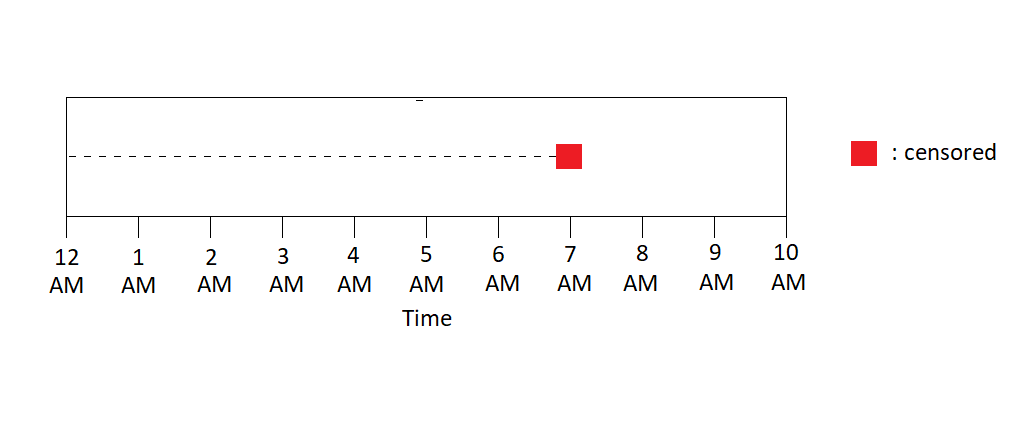
\includegraphics[width=1\linewidth]{figures/left_censoring_example_fix} 

}

\caption{Left Censoring Example}\label{fig:leftcensoringexample}
\end{figure}
In contrast with right censoring, left censoring is a specific instance of censoring in which we only know that the true value of a data point falls below a certain threshold which we call the \emph{limit of detection} (LOD).

To understand this concept better, consider the following example. Imagine a scenario in which you are attempting to estimate the time at which the sun rises each morning. You plan to wake up every morning far before the sun rises, but on the first day of the study, you oversleep and wake up at 7:00 A.M. with the sun already out. We now have an instance of left-censored data. We want to know the time at which the sun rose, but all we have is an upper limit (7:00 A.M.).

Left censoring is commonly found in environmental, water quality, and chemical-related research where the focus is on the concentration of an analyte. Due to limitations on measuring instruments, left censored data are commonly found in these types of studies. The most pressing issue of left-censored data mostly lie in the difficulty of distinguishing between extremely low values and statistical noise (Hall, Perry, \& Anderson, 2020).

\hypertarget{interval}{%
\subsection{Interval Censoring}\label{interval}}
\begin{figure}

{\centering 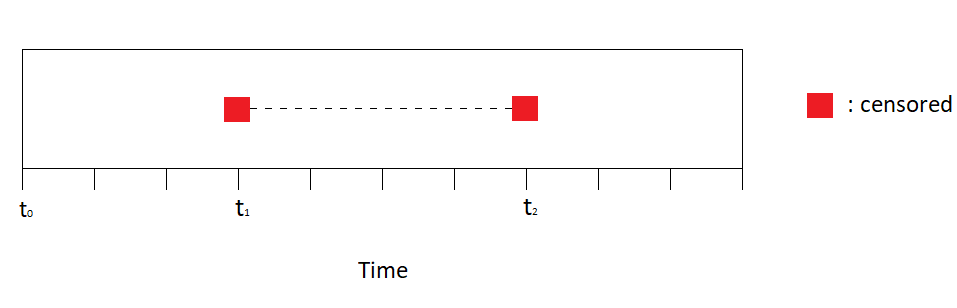
\includegraphics[width=1\linewidth]{figures/interval_censoring_example_fix} 

}

\caption{Interval Censoring Example}\label{fig:intervalcensoringexample}
\end{figure}
Interval censoring is another form of censoring in which the random variable of interest is known to be between an interval of two values. Considering a random variable \(T\), which denotes the survival time of interest, if interval censoring is at hand, we can denote the interval containing \(T\) to be \(I = [t_1, t_2]\), with \(t_1\) being the beginning of the interval and \(t_2\) being the end of the interval. Left and right censoring are special cases of interval censoring. In the case of left censoring, \(t_1 = 0\); and conversely in the case of right censoring, \(t_2 = \infty\).

To conceptualize interval censoring, we can consider a example study on virus testing in which participants get their blood drawn in order to detect whether or not they test positive for a virus or not. The random variable in question is \(T\), which represents the exact timepoint at which the subject contracted the virus. If an individual was first tested at time \(t_1\) and tested negative, but was tested again at a later time \(t_2\) and tested positive, the specific time \(t\) at which the subject contracted the virus is unknown. All we know is that it lies somewhere between the interval, \(I = [t_1, t_2]\), but not the exact time at which they contracted it.

The focus of my thesis deals specifically with the challenges of reporting and working with left-censored data.

\hypertarget{challenges}{%
\section{Challenges of Reporting Censored Data}\label{challenges}}

There is no universal reporting practice for values below the LOD which can lead to confusion amongst researchers. The lack of standardization makes it difficult to distinguish values below the LOD and uncensored values. This can lead to values below the LOD unintentionally being overlooked, causing faulty analysis or conclusions which are heavily flawed.

In a study involving the precision of lead measurements near concentrations of the limit of detection, Berthouex (1993) discusses the disparity among chemists regarding practices involving the recording values below the LOD. He enumerates the following list.
\begin{enumerate}
  \item Reporting the letters ND, "not detected"
  \item Reporting the numeric value of the LOD
  \item Reporting "< LOD", where LOD is the numeric value of the LOD 
  \item Reporting some value between 0 and the LOD, such as one-half the LOD
  \item Reporting the actual measured concentration, even if it falls below the LOD
  \item Reporting the actual measured concentration, followed by "(LOD)" 
  \item Reporting the actual measured concentration with a precision ($\pm$) statement
\end{enumerate}
According to Gilbert (1987), the latter three methods are the best procedures to follow, especially from a practical and statistical point of view. He argues that assuming the small concentration values are not from some sort of measurement error during data collection, then the measured concentration holds value. As such, recording a measurement as ``below LOD'' without any sort of accompanying value would be discarding useful information which could have been used in practice and analysis.

Berthouex (1993) discusses the prevalence in regards to the practice of censoring data by reporting only values which are above the detection limit and discarding those which fail to yield quantifiable results. In the study he conducted, five laboratories were assigned tasks to measure samples of a certain solution. The laboratories were not given information regarding the intent of the study, but a general statement that the concentrations being measured were of ``low'' concentrations. All but one laboratory recorded the actual measured concentrations even though they fell below the LOD. Fortunately, the original measurements for the laboratory that did not report values for all samples were maintained and able to be recovered. Berthouex (1993) stresses the importance of standardization in reporting practices for laboratories and suggested reporting all measurements accompanied with some precision statement, so that data is not lost.

Further supporting the stance of keeping all concentration measurements rather than only those above the detection limit, Monte-Carlo experiments were conducted by Gllllom, Kirsch, Gilroy, \& Survey (1984) to investigate trend-detection for water-quality data. Trend detection is the practice of determining whether the values of a random variable generally increase or decrease over a period of time. They found a general relationship of decreasing trend detection percentages with increased censoring levels, attributing this to the limited availability of information in censored data.

\hypertarget{Approaches}{%
\section{Parameter Estimation Techniques for Left-Censored Data}\label{Approaches}}

It is important to note that the values below the LOD still contain information, specifically that the values is between the lower bound value (if it exists) and the LOD (Chen et al., 2011). As such, there are a variety of statistical treatments to handle censored data which have been popularized in the statistical literature.

Before we discuss the techniques which have been popularized through literature and studies regarding parameter estimation with left-censored data, it important to discuss \emph{omission}, the deletion of data points which are deemed to be invalid as a result of left-censoring or any other deficiencies in the data. As a result of being simple to comprehend and implement, omission is a common technique used in lieu of specialized techniques designed to handle missing data.

One type of omission is known as \emph{available-case analysis}, in which statistical analysis is conducted while only considering the observations which have no missing data on the variables of interest, and excluding the observations with missing values (May, 2012). May argues against this approach and claims that the loss of information from discarding data and the inflation of standard errors of estimates (when discussing missingness in a regression context) will invariably be inflated as a result of the decreased sample size.

Over the past century, a myriad of methods to deal with censoring have been developed to counter this issue of discarding data with omission-based techniques -- some more statistically sound than others. We will review some of the more common methods to estimate descriptive statistics involving censored data, which include: substitution, maximum likelihood estimation, Kaplan-Meier, and regression on order statistics.

\hypertarget{Substitution}{%
\subsection{Substitution Method}\label{Substitution}}

The first technique we will discuss is the substitution method, which involves imputing in a replacement value in lieu of the censored data point. As a method commonly condemned in papers as a statistically unsound method to handle censored data, substitution methods are ubiquitous in the chemical and environmental sciences (Canales, 2018).

Substitution techniques are easy to understand and to implement, akin to the omission techniques we discussed previously. Observations for which measurements fall below the LOD are replaced with a replacement value, which is non-specific and can vary between studies. A non-exhaustive list of common replacement values include: \(\frac{LOD}{2}, \frac{LOD}{\sqrt2}\), and the \(LOD\) itself (Lee \& Helsel, 2005).

Proponents of the substitution method claim that the replacement value \(\frac{LOD}{2}\) is useful for data sets in which the majority of the data are below the LOD or when the distribution of the data is highly skewed; the definition of ``highly skewed'' being any distribution with a geometric standard deviation (a measure of spread commonly used in tandem with log-normal distributions) of 3 or more (Hornung \& Reed, 1989). They also suggest using \(\frac{LOD}{\sqrt2}\) when there are only a few data points below the LOD or when the data is not highly skewed.

Regardless of which replacement value is used, once a dataset is generated containing these replacement values, analysis continues as is, utilizing this new dataset.

As mentioned previously, contention between whether this method is statistically sound or not remains to the present day. The lack of a global, standardized replacement value to substitute is one of the most pronounced downsides of this method. Different disciplines have their own suggested ``best'' replacement value to use, an example being \(\frac{3}{4}\) times the LOD being a common replacement value in geochemistry (Crovelli, 1993). Due to the lack of standardization, many regard substitution techniques as a non-rigorous, statistically unsound method for handling left-censored data (Chen et al., 2011).

Lee \& Helsel (2005) also provides a critique on substitution methods and claim that they can often introduce a ``signal'' which was not originally present within the data, or even obstruct an actual signal which was originally present in the data -- leading to misleading and/or inaccurate results. Supporting Lee \& Helsel (2005)'s claim, Glass and Gray (2001) found the substitution method to introduce large errors and biases when calculating descriptive statistics of interest with left-censored data. Thompson and Nelson (2001) conducted a study in which they found similar results, in that it often led to biased parameter estimates and ``artificially small standard error estimates.'' Hewett and Ganser (2007) also found in their simulation study that the substitution method yielded the lowest average bias and root mean squared error values (comparison metrics to measure accuracy) in their estimation of the mean. Overall, the overall consensus seems to advise against the practice of these substitution techniques.

\hypertarget{MLE}{%
\subsection{Maximum Likelihood Estimation}\label{MLE}}

Maximum likelihood (ML) estimation is a parametric technique which allows us to estimate the parameters of a model when the data are from a known distribution.

Let the random variables \(X_i, \cdots, X_n\) be independent and identically distributed with probability function \(f(x_i|\theta)\), where \(\theta\) is the parameter we are interested in estimating.

For every observed random sample \(x_1,\cdots,x_n\), the joint density function is:

\[f(x_1,...,x_n|\theta) = f(x_1|\theta)...f(x_n|\theta) = \prod_{i=1}^{n}f(x_i|\theta)\]

Our goal is to find the value of \(\theta\) which is most likely to generate our observed data. In order to solve this inverse problem, we introduce the likelihood function, which is defined as a function of the parameter given the observed data:

\[L(\theta) = L(\theta|x_i, \cdots, x_n) = \prod_{i=1}^{n}f(x_i|\theta)\]
Our \emph{maximum likelihood estimate} of our parameter \(\theta\), then, is the value \(\hat{\theta}\) that maximizes the likelihood function, \(L(\theta)\).

When left censoring is present, the likelihood function changes in order to account for both the censored observations and the uncensored observations. We define \(F(x_i|\theta)\) to the cumulative distribution function for our RVs conditioned on \(\theta\). Our new likelihood function when left censoring is present is:

\[lik(\theta) = \prod_{i=1}^n f(x_i|\theta)^{\delta_{i}} \ \times F(x_i|\theta)^{1-{\delta_{i}}}\]

\noindent where \(\delta_{i}\) indicates whether or not the \(i\)th observation is censored:

\[\delta_i =
\begin{cases}
  0 & \text{if censored} \\
  1 & \text{if uncensored}
\end{cases}\]
It is then possible to follow typical procedures to find the maximum likelihood estimates of the parameteres of interest (mean, variance, etc.) from our censored data.

Yavuz, Tekindal, \& Dog (2017) discusses the usage of ML estimation when missing data is present, and notes it is only appropriate for non-negative probability distributions such as the exponential, log-normal, and Weibull models. This is one limitation of ML estimation, it cannot be applied for data which do not fit a specified model -- and is very limited in scope.

ML estimation is one of the most well-known parametric approaches to handling left-censored data. Many studies use ML estimation as a baseline method of handling censored values, to which they compare their new techniques (Ganser \& Hewett, 2010). Despite its prevalence, ML estimation has its weaknesses. Canales (2018) found that the ML estimation seems to underperform when the data in question was highly skewed, producing overinflated mean squared errors. Additionally, because ML estimation is so heavily dependent upon distributional assumptions, an incorrect specification of the distribution of the censored data will inevitably lead to misleading results (Bolks, DeWire, \& Harcum, 2014). Regardless of these limitations, it is a definite staple in the field of parameter estimation with regards to censored data.

\hypertarget{rkm}{%
\subsection{Kaplan-Meier Method}\label{rkm}}

As a phenomenon, censoring is most often discussed in survival analysis, which concerns itself with techniques to analyze a \emph{time to an event} variable. As its name suggests, these variables measure the time which passes until some event of interest occurs. This can be as innocuous as the time until a device breaks, time until birds migrate away from their homes, time until a person passes away, etc. In all cases, there is a possibility of the data being censored.

The Kaplan-Meier (KM) method is a common nonparametric technique used to deal with censored data. Nonparametric methods do not make assumptions about the underlying distribution of the data. The KM method was originally developed to handle right-censored survival analysis data (Hall, Perry, \& Anderson, 2020). The advantages of the KM method lies in its robustness as a nonparametric method -- it performs well without having to depend upon distributional assumptions. Many recommend its usage in cases of severe censoring, instances where more than 90\% of the data is censored (Canales, 2018).

The KM-estimator is a statistic used to estimate the survival curve from the data while accounting for censoring. It does this by assuming that censoring is independent from the event of interest and that survival probabilities remain the same in observations found early in the study and those recruited later in the study (Gillespie et al., 2010).

The KM-estimator of the survival curve at time \(t\) is:

\[\hat{S}(t) = \prod_{\ t_i \le \ t }\left(1-\frac{d_i}{n_i}\right)\]

where \(t_i\) is the distinct event time, \(d_i\) is the number of event occurrences at time \(t_i\), and \(n_i\) is the number of followup times (\(t_i\)) that are greater than or equal to \(t_i\) (how many observations in sample survived until at least time \(t_i\)) (Klein \& Moeschberge, 2003).

Typically, the KM-estimator is used to estimate the distribution function of right-censored data. Helsel (2005, as cited in Yavuz et al., 2017) provided a simple modification of the KM-estimator to allow for the estimation of the survival curve with left-censored values. In his implementation, he ran the left-censored data through a transformation algorithm before using the KM method to change them into right-censored data.

The transformation algorithm works as follows: First, all the left-censored values in the dataset are arranged in descending order of magnitude. Then these left-censored values are subtracted from \(M\), to get \(M-x_i\), the newly transformed, right-censored value (\(M\) is a constant bigger than the maximum value in the dataset). Finally, the non-censored values and the newly transformed values are then arranged in ascending order to be used to estimate the survival function through the Kaplan-Meier estimator.

The KM-method is not an imputation procedure, but instead an estimation technique that allows for the calculation of descriptive statistics for left-censored datasets. She (1997) gives the expressions to calculate the estimated mean, median, and variance:
\begin{table}[h]
\begin{tabular}{ll}
\textbf{Descriptive Statistic} & \textbf{Expression}                                                                                              \\
Mean ($\hat{\mu}$)             & $\hat{\mu} = \displaystyle \int_{0}^{\infty} \hat{S}(t) \ dt$                                                    \\
Median ($\hat{M}$)             & $\hat{M} = \displaystyle \hat{S}^{-1} \left (\frac{1}{2} \right)$                                                              \\
Variance ($Var(\hat{\mu}$)     & $Var(\hat{\mu}) = \displaystyle \sum_{i=1}^{r} \left( \int_{t_i}^{\infty}\hat{S}(t) \ dt \right)^2 \frac{d_i}{n_i(n_i - d_i)}$
\end{tabular}
\end{table}
\hypertarget{ROS}{%
\subsection{Regression on Order Statistics}\label{ROS}}

Lastly, regression on order statistics (ROS) combines both the parametric nature of the MLE approach and nonparametric nature of the KM method. ROS is a semi-parametric method which assumes an underlying distribution (usually lognormal) for the censored measurements but makes no assumption towards the distribution of uncensored measurements.

Environmental Protection Agency (2009) provides a a more detailed explanation to the methodology of ROS, but the basic procedures will be outlined in this thesis.

A brief explanation as to how ROS works is as follows. ROS begins with the estimation of the cumulative probability associated with each distinct LOD. This cumulative probability is distributed equally between the censored values with a common LOD. Once the censored values are ranked, a linear regression model is fit between the uncensored values and the distributional z-scores from the censored probability plot. The parameters of the regression model (slope and intercept of the regression line) is then used to estimate the mean and standard deviation of the distributional model which are then used to generate imputed values for the censored observations.

Delving into the mathematics behind this procedure, we need to first define several variables.

We define \(k\) be the number of distinct LOD values in the data, \(A_i\) as the number of uncensored values between the \(i\)th and \((i+1)\)th LOD for \(i=1\) to \(k-1\), and \(A_k\) as the number of uncensored values above the highest LOD, \(A_0\) as the number of uncensored values below the lowest LOD.

We also define \(B_i\) as the total number of observations (both uncensored and censored) with values below the \(i\)th LOD and \(B_0 = 0\).

We can then write the number of uncensored values below the \(i\)th LOD (\(C_i\)) as:

\[\textrm{Eq. 1.1:} \ \  C_i = B_i - B_{i-1}-A_{i-1}\]

for \(i = 1\) to \(k\).

We can also calculate what is known as the \emph{exceedance probability} (\(pe_{i}\)) for each of our \(k\) LOD values, which represents the proportion of the data greater than or equal to each distinct LOD:

\[\textrm{Eq. 1.2:} \ \  pe_i = pe_{i+1} + \frac{A_i}{A_i+B_i}(1 - pe_{i+1})\]
where \(pe_i\) is the proportion of the data which exceeds the \(i\)th LOD.

Once we obtain exceedance probabilities for each of our distinct LOD values, we compute the plotting positions, aka. the cumulative probabilities, for each of our uncensored values between the \(i\)th and \((i+1)\)th LOD values with the following equation:

\[\textrm{Eq. 1.3:} \ \  pu_{ij} = (1-pe_i)+(\frac{j}{A_i+1})*(pe_i-pe_{i+1})\]

for \(j = 1\) to \(A_i\) and for \(i = 0\) to \(k\).

We also similarly compute the plotting positions for our censored values with:

\[\textrm{Eq. 1.4:} \ \  pc_{ij} = (\frac{j}{C_i+1})*(1-pe_i)\]

for \(j = 1\) to \(C_i\) and for \(i = 1\) to \(k\).

Having defined the relevant variables and equations, we can detail a step-by-step algorithmic procedure on how the ROS method works.
\begin{enumerate}
\def\labelenumi{\arabic{enumi}.}
\item
  Given a dataset with \(n\) observations, identify and sort the \(k\) distinct LOD values.
\item
  Compute \(A_0\), \(A_k\), \(A_i\)'s for \(i=1\) to \(k-1\), and \(B_i\) for \(i=1\) to \(k\).
\item
  Use Eq. 1.1 to compute \(C_i\) for \(i=1\) to \(k\).
\item
  Let \(pe_0 = 1\) and \(pe_{k+1} = 0\). Use Eq. 1.2 to compute \(pe_i\) for \(i=1\) to \(k\).
\item
  Sort all \(pe_i\) from \(i=1\) to \(k\). Use Eq. 1.3 to compute \(pu_{ij}\).
\item
  Compute normal quantiles (z-scores) by computing \(z_{ij}^{d} = \Phi^{-1}(pd_{ij})\), where \(\Phi^{-1}\) is the inverse standard normal CDF.
\item
  Construct censored probability plots using the z-scores from step 6.
\item
  Plot \(z_{ij}^{d}\) against a transformation, \(f(\cdot)\), (ex: log, square root, inverse, etc.) of the uncensored values \(x_{ij}^{d}\).
\item
  Compute correlation coefficient between the \(z_{ij}^{d}\) and \(f(x_{ij}^{d})\) pairs. The transformation which yields the highest correlation coefficient is the one which most optimizes the left-censored values.
\item
  Compute a linear regression of the transformed values, \(f(x_{ij}^{d})\) against the z-scores, \(z_{ij}^{d}\).
\item
  Use Eq. 1.4 to compute \(pc_{ij}\) and repeat steps 6 through 8, to obtain z-scores for the censored values.
\item
  Obtain the transformed imputed values using the slope and intercept from the regression model in step 10 and the censored z-scores from step 11 using the following expression:
\end{enumerate}
\[f(\hat{x}_{ij}^c) = {Intercept} \ + Slope \ * z_{ij}^{c}\]
\begin{enumerate}
\def\labelenumi{\arabic{enumi}.}
\setcounter{enumi}{12}
\tightlist
\item
  Combine the transformed imputed values for the censored values with the transformed uncensored values to obtain estimates for the population mean and standard deviation as normal.
\end{enumerate}
There are of course, also limitations to the ROS method. In order for ROS to be utilized, there needs to be at least 5 known values and more than half the values within the censored variables must be known. As regression is utilized in this method, the response variable must also be a linear function of the explanatory variable (quantiles). Additionally, the errors should have constant variance (Lee \& Helsel, 2005).

We have now covered

\hypertarget{simulations}{%
\chapter{Simulations}\label{simulations}}

Having discussed the various methods to handle left-censored data in the previous chapter, we now turn to a simulation study in order to evaluate the strengths and weaknesses of each method in cases of differing censoring rate, sample size, and distribution. We will also discuss the implementation of the methods, data generating mechanisms, and specific evaluation metrics to assess the performance of each method.

\hypertarget{aims}{%
\section{Aims}\label{aims}}

The question of which method is the best to use is frequently discussed topic within the field. Many studies have been conducted over the years to evaluate the performance of these methods to handle left-censored data, with the results being widely varied and largely inconclusive. First and foremost, a large issue comes in that every conducted study widely differs in the methods being investigated and the scope of the study. As an example of the broad differences between studies which can make comparisons difficult, (Antweiler, 2015) evaluates the effectiveness of 11 different methods with several censoring rates and distributional assumptions, using the median absolute deviation (MAD) as their performance metric of choice. Meanwhile, (Hall, Perry, \& Anderson, 2020) focuses instead on the applications of such methods from a water-quality focused context and investigates the performance of the four methods used in this thesis while disregarding distributional assumptions and censoring rates.

As each of these studies are concerned with their own goals -- specifics of their study will inevitably be different. Studies that are more focused on a general, broad audience, with no assumptions as to what sort of data the individual is working with -- may find more use with the conclusion and results that investigators like Antweiler come up with. There may also be individuals who are more focused on the performance of such methods in a specific context, as in the study conducted by Hall. There is no common ground between statisticians on the optimality of methods, prompting our own foray into this topic. I wish to incorporate the detailed specifications of a simulation study, in essence, taking into consideration distributional parameters of the data-generating mechanism, censoring rates, and sample sizes for each run, while also keeping it applicable to our case-study specific data.

With our simulation study, we wish to identify settings where a method can be effective but also those in which the methods may not be able to perform quite as well. Several investigators in this field have found issues with certain methods underperforming under certain conditions, and brings up the possibility of particular methods being more equipped than others to deal with different rates of censoring. To provide an example of an instance when investigators have found a certain method to perform better than others, we can take a look at Canales (2018)'s study on methods to handle left-censored microbial risk assessment. They found that the substitution method seemed to work much better than expected while other methods, such as the MLE method, seemed to have trouble when applied to highly skewed data. Meanwhile Antweiler (2015)'s report suggest that regardless of the method or sample size, obtaining reliable estimates from datasets where censoring was greater than 40\% was unfeasible.

Claims regarding the effectiveness of methods with regards to censoring rates, distribution of data, and sample size are all highly contentious. In order to get a better idea of sense of how these claims hold up, our goal is to evaluate the validity of those claims by conducting a simulation study of our own to put these methods into practice. We expect the results of our simulation study to largely depend on how we specify our data generating mechanism, which will be discussed shortly.

\hypertarget{data_generating_mechanisms}{%
\section{Data-Generating Mechanisms}\label{data_generating_mechanisms}}

The data generated for use in our study will be obtained by using parametric draws from user-specified distributions (log-normal, exponential, and Weibull), as the methods utilized can only be used with non-negative distributions (Yavuz, Tekindal, \& Dog, 2017). Our data-generating mechanism also alters criterion such as the sample size, \(n_{obs} = \{10, 100, 1000\}\) and censoring rate, \(R = \{0.10, 0.30, 0.50\}\). In the following sections, we will often interchangeably use ``small, medium, large'' and ``low, medium, and high'' to differentiate between the different values for sample size and censoring rate, respectively. For example, ``small sample size'' is equivalent to \(n_{obs} = 10\) and ``high censoring rate'' is equivalent to \(R = {0.50}\).

We begin by generating draws from a specified distribution of size \(n_obs\), and then determine our censored values by arranging the uncensored observations in ascending order, and then setting those in the lowest \(100R \ \%\) to be censored. If the censoring rate were to be \(R = 0.10\), the lowest 10\% of the observations will be marked as censored while the rest remain uncensored.

\newpage

\hypertarget{estimands}{%
\section{Estimands}\label{estimands}}

Each of the four methods discussed in the previous chapter are designed for usage in obtaining summary statistics for left censored data (Shoari, 2018). In our simulation study, we will be using the sample mean as an estimator for our estimand, the population mean, \(\mu\).

\hypertarget{performance_measures}{%
\section{Performance Measures}\label{performance_measures}}

Morris, White, \& Crowther (2019) define performance measures as numeric metrics used to assess the performance of the method in question. The criterion we will use to assess the performance of each of our four methods will consist of: bias, variance, and mean squared error (MSE).

\hypertarget{variance}{%
\subsection{Variance}\label{variance}}

Prior to defining variance, we must discuss the concept of \emph{precision}. Precision simply refers to how far away estimates from different samples are from one another. Low precision indicates that the estimates from each sample are far from one another in value, while high precision indicates the opposite. Knowing this, \emph{variance} is a metric which informs us on the precision of an estimator. It is defined as the average squared deviation of the estimator from its average:

\[Variance = E[(\hat{\mu}-E(\hat{\mu}))^2]\]

Estimators with low variances generally remain close in value throughout all samples, while those with high variance may wildly differ between samples. It is generally preferable to have an estimator with low variance. Precision measurements, such as the variance, are not a sole indicator of an estimator's performance (Walther \& Moore, 2005). While useful for assessing how close values are to one another, it is just as important to obtain the estimator's \(bias\), a measure of how close the obtained estimate is to the true value.

\hypertarget{bias}{%
\subsection{Bias}\label{bias}}

The next performance metric which we will use is bias, which is defined as the difference between an estimator's expected value and the true value of the parameter. In our case, we are using the estimator \(\hat{\mu}\) to estimate the true population mean, \(\mu\), in each of our samples. The formal definition of bias is as follows:

\[Bias = E(\hat{\mu}) - \mu\]

Bias informs us on the difference of the estimator from the true parameter. A natural question to ask is often whether if an estimator is any ``good.'' One possible measures of this idea ``good,'' naturally comes in the idea of an unbiased estimator. If the bias of an estimator were to be equal to zero, we would define the estimator to be \emph{unbiased}, meaning that the estimator produces parameter estimates which are on average, equal to the true value.

An estimator being unbiased does not necessarily equate to it being ideal. An unbiased estimator could have high variance, which would mean that the estimator in each sample would be significantly different from one another, but on average -- they equal the true population estimand.

On the opposite hand, it would also not be very useful if an estimator had low variance but high bias. This would mean that each sample would consistently produce similar estimates which are very far from the true population estimand.

\hypertarget{mean-squared-error-mse}{%
\subsection{Mean Squared Error (MSE)}\label{mean-squared-error-mse}}

Evidently we do not want our estimator to be too biased nor too variant. This conflict is known as the \emph{bias-variance tradeoff}, a dilemma in which we can never simultaneously minimize the bias and variance of our estimator.

While we generally would like estimators which have low bias and low variance, it can be difficult to achieve both at once. As such, it is common to instead turn to a quantity known as the \emph{mean squared error} (MSE), which is a quantitative measurement used to assess the accuracy of an estimator. The MSE measures how far away, on average, an estimator is from its true value and makes use of both bias and variance in its calculations. The formal definition of MSE is:

\[MSE = E[(\hat{\mu} -\mu)^2] = Var(\hat{\mu})+[Bias(\hat{\mu})]^2\]

We can show that the MSE of estimator can be rewritten in terms of its variance and bias:

\[E[(\hat{\mu} -\mu)^2] = E(\hat{\mu}^2) + \mu^2 - 2E(\hat{\mu})\mu\]
From \(Bias = E(\hat{\mu}) - \mu\), it follows that:

\[Bias^2 = E^2(\hat{\mu}) +\mu^2 -2E(\hat{\mu})\theta\]

From \(Variance = E[(\hat{\mu}-E(\hat{\mu}))^2] = E(\hat{\mu}^2) - E^2(\hat{\mu})\), we can combine the square of the bias with variance, which yields:

\[Bias^2 + Var = [E^2(\hat{\mu}) +\mu^2 -2E(\hat{\mu})\theta] + [E(\hat{\mu}^2) - E^2(\hat{\mu})]\]

The \(E^2(\hat{\mu})\) terms cancel out, and we are left with:

\[E^2(\hat{\mu}) +\mu^2 -2E(\hat{\mu})\theta = E[(\hat{\mu} -\mu)^2] = Bias\]

As the MSE is always positive, MSE values closer to zero are more desirable -- as it is an indicator that the estimator is accurate.

\hypertarget{results}{%
\section{Results}\label{results}}

The results of our simulation study are presented in the following tables below.
\begin{table}

\caption{\label{tab:unnamed-chunk-1}Performance metrics of our our 
             4 methods with data derived from the log-normal 
             distribution with mean = 1 and SD = 0.5.}
\centering
\fontsize{11.5}{13.5}\selectfont
\begin{tabular}[t]{lrrrrr}
\toprule
  & Sample Size & Avg. Mean & Bias & Variance & MSE\\
\midrule
\addlinespace[0.3em]
\multicolumn{6}{l}{\textbf{Censoring Rate = 0.1}}\\
\hspace{1em}km & 10 & 1.009 & 0.00924 & 0.02289 & 0.02295\\
\hspace{1em}mle & 10 & 0.997 & -0.00262 & 0.02276 & 0.02275\\
\hspace{1em}ros & 10 & 0.991 & -0.00923 & 0.02190 & 0.02197\\
\hspace{1em}substitution & 10 & 0.981 & -0.01901 & 0.02201 & 0.02235\\
\hspace{1em}km & 100 & 1.008 & 0.00766 & 0.00263 & 0.00268\\
\hspace{1em}mle & 100 & 0.998 & -0.00178 & 0.00263 & 0.00263\\
\hspace{1em}ros & 100 & 0.999 & -0.00142 & 0.00258 & 0.00258\\
\hspace{1em}substitution & 100 & 0.983 & -0.01707 & 0.00255 & 0.00284\\
\hspace{1em}km & 1000 & 1.009 & 0.00913 & 0.00024 & 0.00033\\
\hspace{1em}mle & 1000 & 1.000 & -0.00004 & 0.00024 & 0.00024\\
\hspace{1em}ros & 1000 & 1.001 & 0.00127 & 0.00024 & 0.00024\\
\hspace{1em}substitution & 1000 & 0.985 & -0.01536 & 0.00024 & 0.00047\\
\addlinespace[1em]
\multicolumn{6}{l}{\textbf{Censoring Rate = 0.3}}\\
\hspace{1em}km & 10 & 1.050 & 0.05015 & 0.02754 & 0.03002\\
\hspace{1em}mle & 10 & 0.968 & -0.03235 & 0.02431 & 0.02534\\
\hspace{1em}ros & 10 & 0.976 & -0.02381 & 0.02374 & 0.02429\\
\hspace{1em}substitution & 10 & 0.937 & -0.06286 & 0.02298 & 0.02691\\
\hspace{1em}km & 100 & 1.049 & 0.04904 & 0.00288 & 0.00528\\
\hspace{1em}mle & 100 & 0.974 & -0.02628 & 0.00252 & 0.00321\\
\hspace{1em}ros & 100 & 1.000 & -0.00001 & 0.00259 & 0.00259\\
\hspace{1em}substitution & 100 & 0.944 & -0.05642 & 0.00241 & 0.00559\\
\hspace{1em}km & 1000 & 1.049 & 0.04939 & 0.00026 & 0.00270\\
\hspace{1em}mle & 1000 & 0.974 & -0.02554 & 0.00024 & 0.00089\\
\hspace{1em}ros & 1000 & 1.004 & 0.00377 & 0.00024 & 0.00025\\
\hspace{1em}substitution & 1000 & 0.945 & -0.05540 & 0.00022 & 0.00329\\
\addlinespace[1em]
\multicolumn{6}{l}{\textbf{Censoring Rate = 0.5}}\\
\hspace{1em}km & 10 & 1.148 & 0.14806 & 0.03718 & 0.05907\\
\hspace{1em}mle & 10 & 0.908 & -0.09188 & 0.02236 & 0.03078\\
\hspace{1em}ros & 10 & 0.967 & -0.03257 & 0.02810 & 0.02914\\
\hspace{1em}substitution & 10 & 0.908 & -0.09229 & 0.02368 & 0.03217\\
\hspace{1em}km & 100 & 1.129 & 0.12867 & 0.00372 & 0.02027\\
\hspace{1em}mle & 100 & 0.904 & -0.09649 & 0.00240 & 0.01171\\
\hspace{1em}ros & 100 & 0.996 & -0.00399 & 0.00316 & 0.00317\\
\hspace{1em}substitution & 100 & 0.904 & -0.09614 & 0.00250 & 0.01174\\
\hspace{1em}km & 1000 & 1.129 & 0.12885 & 0.00035 & 0.01695\\
\hspace{1em}mle & 1000 & 0.905 & -0.09535 & 0.00023 & 0.00932\\
\hspace{1em}ros & 1000 & 1.005 & 0.00515 & 0.00029 & 0.00032\\
\hspace{1em}substitution & 1000 & 0.905 & -0.09484 & 0.00023 & 0.00923\\
\bottomrule
\end{tabular}
\end{table}
\begin{table}

\caption{\label{tab:unnamed-chunk-2}Performance metrics of our our 3 
             methods (MLE method absent) with data derived from the 
             exponential distribution with a shape parameter = 1.}
\centering
\fontsize{11.5}{13.5}\selectfont
\begin{tabular}[t]{lrrrrr}
\toprule
  & Sample Size & Avg. Mean & Bias & Variance & MSE\\
\midrule
\addlinespace[0.3em]
\multicolumn{6}{l}{\textbf{Censoring Rate = 0.1}}\\
\hspace{1em}km & 10 & 1.012 & 0.01191 & 0.06330 & 0.06341\\
\hspace{1em}mle & 10 &  &  &  \vphantom{2} & \\
\hspace{1em}ros & 10 & 0.997 & -0.00265 & 0.06173 & 0.06170\\
\hspace{1em}substitution & 10 & 0.992 & -0.00761 & 0.06186 & 0.06189\\
\hspace{1em}km & 100 & 1.010 & 0.00974 & 0.00646 & 0.00656\\
\hspace{1em}mle & 100 &  &  &  \vphantom{2} & \\
\hspace{1em}ros & 100 & 1.005 & 0.00469 & 0.00647 & 0.00648\\
\hspace{1em}substitution & 100 & 0.994 & -0.00553 & 0.00649 & 0.00652\\
\hspace{1em}km & 1000 & 1.007 & 0.00693 & 0.00067 & 0.00072\\
\hspace{1em}mle & 1000 &  &  &  \vphantom{2} & \\
\hspace{1em}ros & 1000 & 1.003 & 0.00308 & 0.00066 & 0.00067\\
\hspace{1em}substitution & 1000 & 0.992 & -0.00798 & 0.00071 & 0.00077\\
\addlinespace[1em]
\multicolumn{6}{l}{\textbf{Censoring Rate = 0.3}}\\
\hspace{1em}km & 10 & 1.063 & 0.06291 & 0.07325 & 0.07717\\
\hspace{1em}mle & 10 &  &  &  \vphantom{1} & \\
\hspace{1em}ros & 10 & 0.991 & -0.00916 & 0.06389 & 0.06394\\
\hspace{1em}substitution & 10 & 0.970 & -0.02978 & 0.06372 & 0.06457\\
\hspace{1em}km & 100 & 1.053 & 0.05270 & 0.00719 & 0.00996\\
\hspace{1em}mle & 100 &  &  &  \vphantom{1} & \\
\hspace{1em}ros & 100 & 1.011 & 0.01140 & 0.00685 & 0.00698\\
\hspace{1em}substitution & 100 & 0.972 & -0.02764 & 0.00717 & 0.00793\\
\hspace{1em}km & 1000 & 1.054 & 0.05368 & 0.00073 & 0.00361\\
\hspace{1em}mle & 1000 &  &  &  \vphantom{1} & \\
\hspace{1em}ros & 1000 & 1.017 & 0.01683 & 0.00085 & 0.00113\\
\hspace{1em}substitution & 1000 & 0.974 & -0.02557 & 0.00152 & 0.00217\\
\addlinespace[1em]
\multicolumn{6}{l}{\textbf{Censoring Rate = 0.5}}\\
\hspace{1em}km & 10 & 1.193 & 0.19309 & 0.10925 & 0.14648\\
\hspace{1em}mle & 10 &  &  &  & \\
\hspace{1em}ros & 10 & 0.992 & -0.00789 & 0.07636 & 0.07638\\
\hspace{1em}substitution & 10 & 0.968 & -0.03151 & 0.07419 & 0.07514\\
\hspace{1em}km & 100 & 1.162 & 0.16154 & 0.00992 & 0.03601\\
\hspace{1em}mle & 100 &  &  &  & \\
\hspace{1em}ros & 100 & 1.023 & 0.02269 & 0.00792 & 0.00844\\
\hspace{1em}substitution & 100 & 0.961 & -0.03925 & 0.00946 & 0.01100\\
\hspace{1em}km & 1000 & 1.163 & 0.16301 & 0.00201 & 0.02858\\
\hspace{1em}mle & 1000 &  &  &  & \\
\hspace{1em}ros & 1000 & 1.036 & 0.03598 & 0.00164 & 0.00293\\
\hspace{1em}substitution & 1000 & 0.964 & -0.03594 & 0.00405 & 0.00534\\
\bottomrule
\end{tabular}
\end{table}
\begin{table}

\caption{\label{tab:unnamed-chunk-3}Performance metrics of our our 3 methods 
             (MLE method absent) with data derived from the Weibull 
             distribution with a shape parameter = 1 and 
             scale parameter = 1.}
\centering
\fontsize{11.5}{13.5}\selectfont
\begin{tabular}[t]{lrrrrr}
\toprule
  & Sample Size & Avg. Mean & Bias & Variance & MSE\\
\midrule
\addlinespace[0.3em]
\multicolumn{6}{l}{\textbf{Censoring Rate = 0.1}}\\
\hspace{1em}km & 10 & 1.010 & 0.00977 & 0.07703 & 0.07710\\
\hspace{1em}mle & 10 &  &  &  \vphantom{2} & \\
\hspace{1em}ros & 10 & 0.997 & -0.00339 & 0.07518 & 0.07516\\
\hspace{1em}substitution & 10 & 0.993 & -0.00678 & 0.07525 & 0.07527\\
\hspace{1em}km & 100 & 1.010 & 0.00998 & 0.00768 & 0.00778\\
\hspace{1em}mle & 100 &  &  &  \vphantom{2} & \\
\hspace{1em}ros & 100 & 1.006 & 0.00626 & 0.00768 & 0.00772\\
\hspace{1em}substitution & 100 & 0.998 & -0.00215 & 0.00768 & 0.00768\\
\hspace{1em}km & 1000 & 1.006 & 0.00625 & 0.00077 & 0.00081\\
\hspace{1em}mle & 1000 &  &  &  \vphantom{2} & \\
\hspace{1em}ros & 1000 & 1.004 & 0.00374 & 0.00077 & 0.00079\\
\hspace{1em}substitution & 1000 & 0.995 & -0.00548 & 0.00081 & 0.00084\\
\addlinespace[1em]
\multicolumn{6}{l}{\textbf{Censoring Rate = 0.3}}\\
\hspace{1em}km & 10 & 1.067 & 0.06660 & 0.08638 & 0.09078\\
\hspace{1em}mle & 10 &  &  &  \vphantom{1} & \\
\hspace{1em}ros & 10 & 0.996 & -0.00440 & 0.07540 & 0.07540\\
\hspace{1em}substitution & 10 & 0.981 & -0.01896 & 0.07526 & 0.07559\\
\hspace{1em}km & 100 & 1.054 & 0.05434 & 0.00845 & 0.01140\\
\hspace{1em}mle & 100 &  &  &  \vphantom{1} & \\
\hspace{1em}ros & 100 & 1.016 & 0.01566 & 0.00804 & 0.00829\\
\hspace{1em}substitution & 100 & 0.982 & -0.01761 & 0.00825 & 0.00856\\
\hspace{1em}km & 1000 & 1.055 & 0.05451 & 0.00085 & 0.00382\\
\hspace{1em}mle & 1000 &  &  &  \vphantom{1} & \\
\hspace{1em}ros & 1000 & 1.021 & 0.02059 & 0.00094 & 0.00136\\
\hspace{1em}substitution & 1000 & 0.984 & -0.01618 & 0.00152 & 0.00178\\
\addlinespace[1em]
\multicolumn{6}{l}{\textbf{Censoring Rate = 0.5}}\\
\hspace{1em}km & 10 & 1.221 & 0.22073 & 0.12826 & 0.17694\\
\hspace{1em}mle & 10 &  &  &  & \\
\hspace{1em}ros & 10 & 1.009 & 0.00898 & 0.08864 & 0.08869\\
\hspace{1em}substitution & 10 & 0.998 & -0.00169 & 0.08642 & 0.08639\\
\hspace{1em}km & 100 & 1.173 & 0.17290 & 0.01172 & 0.04162\\
\hspace{1em}mle & 100 &  &  &  & \\
\hspace{1em}ros & 100 & 1.033 & 0.03267 & 0.00934 & 0.01040\\
\hspace{1em}substitution & 100 & 0.980 & -0.01968 & 0.01051 & 0.01090\\
\hspace{1em}km & 1000 & 1.173 & 0.17294 & 0.00201 & 0.03192\\
\hspace{1em}mle & 1000 &  &  &  & \\
\hspace{1em}ros & 1000 & 1.045 & 0.04497 & 0.00165 & 0.00367\\
\hspace{1em}substitution & 1000 & 0.982 & -0.01751 & 0.00372 & 0.00402\\
\bottomrule
\end{tabular}
\end{table}
From the results of our simulation study, we can see that with the data generated from the log-normal distribution, in the case of low censoring (0.10), when dealing with sample sizes of 10 and 100, the methods are largely comparable to one another. Substitution and KM do not perform quite as well as ROS and MLE, both displaying an increase in absolute bias and MSE when compared to the latter two. Substitution performs significant worse than KM. MLE and ROS perform rather equally well in all sample sizes for low-censoring.

When considering medium censoring (0.30), much of the same observations still hold true. Substitution performs the worse, followed by KM. MLE and ROS both perform well. However, ROS has a slight edge over MLE, especially as sample sizes increase, attaining lower MSE values than the latter.

All four methods begin to perform worse when the censoring rate is increased to 0.5, which is to be expected. As more and more missingness is introduced within the dataset, it becomes more difficult to obtain accurate estimates for all methods. Once again, substitution and KM attain high absolute bias and MSE values. However, it is now KM which performs worse than substitution in the setting of high censoring. Similarly to before, albeit being more noticeable now, ROS performs better than MLE with all sample sizes.

We can see with the exponential and Weibull cases, all three methods perform equally well in the case of low (0.10) censoring with all sample sizes, obtaining similar bias and MSE values across all sample sizes for both the exponential and Weibull datasets. KM consistently performs the worst with with medium (0.30) and high (0.50) censoring when compared to the other methods across all sample sizes. In these censoring settings, it is also the case that ROS performs the best with substitution not far behind.

In summary, regardless of distributional assumptions all of the methods perform well when censoring is low, with very minute differences in performance metrics. KM does not perform well in the lognormal distribution with high censoring rates and struggles in the exponential and Weibull cases with medium and high censoring rates. While MLE was only used in the case of the lognormal data, it also performs quite well, although not quite as well as ROS. ROS performed the best in the case of medium and high censoring across all 3 distributions.

\hypertarget{discussion}{%
\section{Discussion}\label{discussion}}

It important to note that while there are a large number of papers which discuss the ideal method or strategy to handle left-censored data,these studies have a large number of differences in censoring rates, distribution used, methods used, and other aspects of design setups which make comparisons regarding the results obtained from the studies quite difficult. As such, descriptions of specifics regarding the study design in the following studies will be omitted as necessary.

Several results from our simulation studies agree with previous findings conducted from other investigators in the field. Gilliom \& Helsel (1986) claims that with the lognormal distribution, the ROS method was superior. This claim is furthered with our own results: we find that the ROS method is rather robust, even with censoring and produces an accurate and precise estimate of the mean in all cases in our simulation study.

Another investigation by Kroll \& Stedinger (1996) found that with regards to a lognormal distribution only, ROS and MLE worked extremely well, with MLE outperforming the other methods especially in highly censored cases. While the MLE method did perform rather well in most cases in our simulation study, it did not outperform the ROS method, which in fact obtained much better estimates of the mean in highly censored settings.

There are of course also studies which offer differing results from the ones we obtained in our simulation study.

Schmoyer, Beauchamp, Brandt, \& Hoffman (1996) compared only MLE and KM and found that the KM method performed nearly as well as the MLE in the case of the lognormal distribution. However, this was not the case in our simulation study. While the KM and MLE methods were able to perform adequately in the case of low (0.1) and medium (0.3) censoring, they performed the worst out of all four methods when dealing with highly censored cases. The censoring rates used in their study consisted of 25\%, 50\%, and 70\% -- which far exceeded the censoring values used in this thesis.

She (1997) conducted a study investigating censored water quality data with the intent of investigating how well the KM method performs with regards to the same methods we utilize in this thesis. The results from She's study showed that KM outperformed all other methods, which contradicts the findings in the simulation study conducted in this thesis. Upon further investigation, the size of the dataset utilized by She consisted of 56 observations from water monitoring stations, in which around 11 were censored (20\% of the dataset). While the KM method is not ideal for highly censored cases from the results of our simulation study, it certainly is able to be used for smaller sample sizes -- which is further supported with She's findings. There may be a difference in how well the methods perform with actual data as compared to simulated data -- which we will investigate in the next chapter.

\hypertarget{limitations}{%
\subsection{Limitations}\label{limitations}}

Shortcomings in the results presented in this study may come from the fact that we generated data with known distributional parameters. It could be the case that the effectiveness of our methods were only due to having such artificial data. Alterations in our study to instead generate data from methods such as randomized pulls from an a real-world dataset of interest via. methods such as bootstrapping could provide different insights. As we discussed previously with the results from She (1997), methods may perform differently when utilized with artificial datasets as compared to real world, left censored data. We do not claim our findings in the simulation study to be representative for all cases of left censored data.

\hypertarget{real_data}{%
\section{Study on Real Data}\label{real_data}}

{[}can write this section after some preliminary exploration with coal groundwater data{]}

\hypertarget{casestudy}{%
\chapter{Case Study}\label{casestudy}}

\hypertarget{background}{%
\section{Background}\label{background}}

Coal is one of the most prevalent combustible fuels being utilized all over the world, as it is one of the easiest methods of obtaining energy due to the abundance of the substance. Generally, coal plants produce electricity by burning coal, which produces coal ash as a byproduct. Over 100 million tons of coal ash are produced every year at these plants, which are then disposed through landfills and waste ponds at these plants. The main concern of ecologists regarding this matter is that the coal ash produced by these plants can often contaminate the local groundwater, leading to toxic contaminants being found in local water sources. Coal ash is dangerous due to its composition, which contains a long list of dangerous chemicals including -- but not limited to: arsenic, radium, boron, and other contaminants which have been found to be toxic to humans and animals alike (Kelderman et al., 2019).

Only recently has there been an increase in the frequency of complaints and concerns regarding the disposing practices of coal plants. This is due to disturbances at coal plants, such as the 2010 Kingston Fossil Plant coal ash incident in Tennessee. This area has become an attractive location in which many sites of ecological studies have been conducted the years following the incident. Leaching experiments conducted by Ruhl, Vengosh, Dwyer, Hsu-Kim, \& Deonarine (2010) has revealed significant levels of dissolved arsenic, boron, strontium, and barium in the water which has been in contact with the coal ash, which they specifically note to be threat to aquatic life in the surrounding area. Prompted by environmental organizations, groups, and individuals alike, an onslaught of pressure was put on the Environmental Protection Agency, which resulted in the Coal Ash Rule being put into effect in 2015 (Kelderman et al., 2019).

This rule has forced over 265 coal plants -- about 3/4 of all coal plants in the US -- to make data regarding chemical concentrations publicly available to the general population. In their analysis using this data, the Environmental Integrity Project (2020), a non-profit organization dedicated to environmental justice issues, have discussed the prevalence of groundwater contamination for in the wells located in these coal related facilities.
\begin{figure}

{\centering 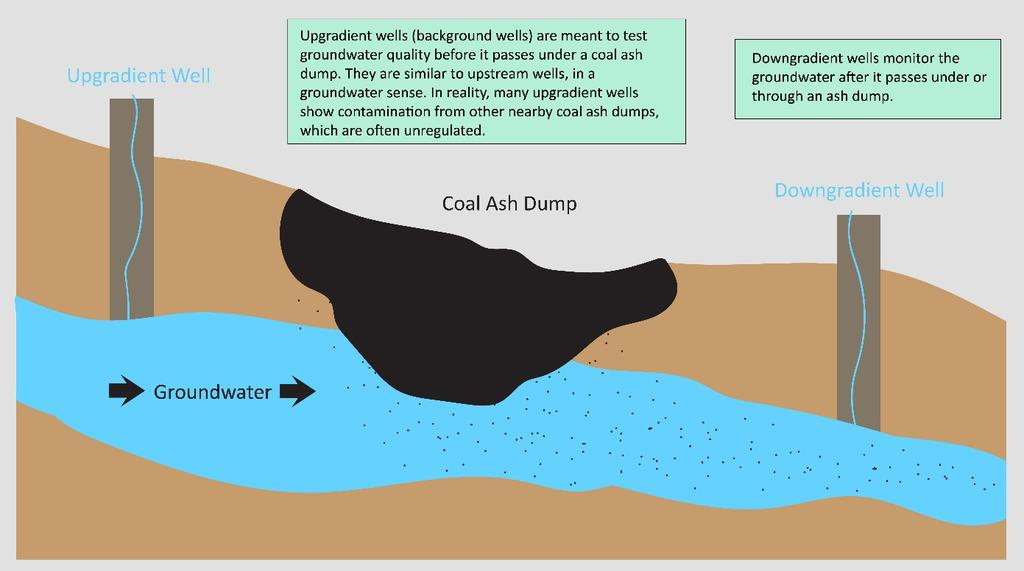
\includegraphics[width=1\linewidth]{figures/upgradientdowngradient} 

}

\caption{Difference Between Upgradient and Downgradient Wells}\label{fig:upgradientdowngradient}
\end{figure}
Typically in a coal ash plant, there exists two types of wells: upgradient wells and downgradient wells. These wells are essential to measure the amount of contamination being caused by coal ash. Upgradient wells, also known as background wells, measures the concentrations of chemicals in groundwater before it passes through an coal ash dump. Conversely, downgradient wells measure the concentrations of chemicals in groundwater after it passes through a coal ash dump. Figure \ref{fig:upgradientdowngradient} is a useful visualization detailing the specifics regarding the differences between the two types of wells. While both types of well are susceptible to contamination through coal ash related means, it is more frequently the case that we focus on the concentrations of downgradient wells as they are good indicators of possible contamination in the water being accessed by the general public.

The goal of the study conducted by Kelderman et al. (2019) was to identify the percentage of coal plants which have unsafe levels of contamination. High concentrations of toxic chemicals are what classify a well as being contaminated or not. More specifically, we obtain the mean concentrations of the contaminant in question for all the wells measuring a specific chemical in a site. If the mean contamination of a contaminant in question, say, arsenic, was above the health-based thresholds set by the EPA, then that well would be marked as an ``exceedance,'' and deemed to be contaminated.

Kelderman et al. (2019) notes the possibility of contamination being caused by an external factor, unrelated to the coal ash, and provides a stipulation as how to account for this. In the process of calculating mean concentrations, they excluded wells in which the mean downgradient values were lower than the mean upgradient values, as this would mean that the contamination was not caused by the coal plant itself. They also exclude upgradient wells in this calculation, as the focus is on possible contamination in downgradient well in the coal plant.

\hypertarget{data}{%
\section{Data}\label{data}}

It is important to note where the data used originated from, before we delve into the details of our case study. As such, a brief history regarding the Coal Ash Rule and its origin will be explored, alongside details regarding our coal ash dataset.

\hypertarget{coalashrule}{%
\subsection{Coal Ash Rule}\label{coalashrule}}

A large coal ash spill at the Tennessee Valley Authority which occurred on December 22, 2008 in Kingston, TN -- prompted the Environmental Protection Agency (EPA) to propose a set of standardized regulations and procedures to address the concerns regarding coal ash plants nationwide in the US. This was known as the Coal Ash Rule, which passed legislation on December 19, 2014 (Environmental Protection Agency, 2020). Over the years, several changes were made to the Coal Ash Rule in the form of amendments. One of these amendments (published on the April 15, 2015) stated that coal plants would be required to publish data regarding the concentrations of contaminants in the wells and other facility information to the general public.

\hypertarget{source-of-data}{%
\subsection{Source of Data}\label{source-of-data}}

The data used in the study are from a collection of results published by each coal plant in their ``Annual Groundwater Monitoring and Corrective Action Reports.'' These reports are coal-specific, in PDF format, and can often be up to thousands of pages long, which makes it difficult for individuals to parse through data in a meaningful way. Due to this inaccessibility, the Environmental Integrity Project (2020) began a long project to parse and wrangle through these reports to compile them into a more accessible machine-readable format. This compilation contains information from over 443 annual groundwater monitoring reports posted by 265 coal ash plants, and is downloadable from the EIP's website. This dataset compiled by the Environmental Integrity Project are what we will utilize in our case study.

\hypertarget{variables}{%
\subsection{Variables}\label{variables}}

The coal dataset contains information regarding chemical concentrations at coal plants. A coal plant consists of multiple disposal areas for the coal ash that it produces. At each disposal area, there are specific locations that groundwater is being measured, known as wells, which represent an observation in the dataset. There are over 265 coal plants, also known as ``sites,'' in this dataset. A single site is divided into multiple subsections, known as ``disposal areas.'' Each well can be associated with a disposal area and subsequently, a site.

Specifics regarding the variables in the coal dataset can be viewed in Table \ref{tab:datadictionary}. Each observation in the dataset represents a well which measures the concentration of the contaminant in question. Most of the variables are explanatory, such as the state, site, and disposal area in which the well is located in. However, there are several variables specific to groundwater data collection which are important to note.

There are four different types that each well can be classified as, which is represented in the \texttt{type} variable. These consist of: \texttt{L}, \texttt{M}, \texttt{SI}, and \texttt{U} which stand for ``landfill,'' ``mixed,'' ``surface-impacted,'' and ``unknown.'' We have already mentioned downgradient and upgradient wells during our discussion of the coal ash rule, but we will provide more detail now. In a groundwater monitoring system it is common to have designated wells for specific purposes. A common approach in a coal site is to have separate wells, upgradient wells, whose purpose is to measure ``natural'' water conditions and downgradient wells, which measures water conditions after it passes through a coal ash disposal area.

Coal plants may also follow different reporting protocols, which necessitates the ``measurement unit'' column. While some contaminants such as radium, are measured only in one unit (pCi/L) -- most others are measured differently across sites. One site may measure arsenic with using milligrams/L while another site uses micrograms/L.

The remaining variables in our dataset are mostly self explanatory, containing information regarding the date when sample was collected, unique ID of the well, and whether if the measurement is below the limit of detection. A data dictionary of all variables in the dataset can be viewed in Table \ref{tab:datadictionary}.
\begin{table}

\caption{\label{tab:datadictionary}Data dictionary for the coal dataset.}
\centering
\begin{tabular}[t]{ll>{\raggedright\arraybackslash}p{7.6cm}}
\toprule
Variable & Variable Name & Description\\
\midrule
State & state & The state where the site is located.\\
\addlinespace
Site & site & The name of the site as it is presented in its
             groundwater monitoring \vphantom{1} report.\\
\addlinespace
Disposal Area & disposal.area & The name of the disposal area(s) as they are presented 
             in the groundwater monitoring report. Note: some wells 
             monitor groundwater from more than one disposal unit.\\
\addlinespace
Type of Well & type & The type of disposal unit. SI = surface impoundment, 
             L= landfill, M = mixed multi-unit (landfill and surface 
             impoundment), and U = unknown.\\
\addlinespace
ID of Well & well.id & The identifier given to each monitoring well in the 
             groundwater monitoring report.\\
\addlinespace
Gradient Type & gradient & The location of the groundwater monitoring well 
             relative to the regulated ash disposal unit it 
             monitors.\\
\addlinespace
Sample Date & samp.date & The date the well was sampled.\\
\addlinespace
Contaminant Name & contaminant & The contaminant name. These have been standardized to 
             allow for analyses across plants.\\
\addlinespace
Measurement Unit & measurement.unit & The concentration units. These include mg/l, ug/l, 
             pCi/l, and standard units (SU) for pH.\\
\addlinespace
Below Detection & below.detection & LOD status for the concentration, '<' indicates that 
             the concentration was below the LOD.\\
\addlinespace
Concentration & concentration & The concentration of the contaminant.\\
\bottomrule
\end{tabular}
\end{table}
\hypertarget{plan-of-action}{%
\subsection{Plan of Action}\label{plan-of-action}}

The investigation conducted by Kelderman et al. (2019) mentions certain restrictions within the data that we believe may have caused their analysis to potentially be inaccurate. The limit of detection problem arises when measuring devices used to measure chemical concentrations are unable to detect below a certain threshold, causing large numbers of observations to be considered ``below detection.'' These values are often encoded as NA or even mistakenly marked as 0.

Our end goal remains the same as the original research question proposed by Kelderman et al. (2019), which is to identify (the top ten most) contaminated coal plants. Around 2/3 of all wells in the dataset have concentrations found to be below the detection limit. This is a significant portion of the data being censored, which we believe may have significant consequences in the results obtained during analysis. Kelderman et al. (2019) handled these censored values by assuming that their concentration was one half of the detection limit. In essence, they employed the substitution method we discussed previously, with a replacement value of \(\frac{1}{2}\) LOD for the values below the detection limit.

The goal of our case study is to employ the techniques we introduced back in chapter 2 to see if they would result in potential differently conclusions. Specifically, we wish to check if the proportion of wells in the U.S. in which contamination is present would be altered if we used our mean estimation techniques to calculate the average concentrations of the contaminants. We would also like to implement a baseline (control) method in which we calculate mean estimates while disregarding the censoring status of the observations and see if our methods truly offer any different conclusions than the claims made by Kelderman et al. (2019) regarding the top 10 most contaminated wells in the U.S.

\hypertarget{application}{%
\section{Application}\label{application}}

\hypertarget{background-tentative-title}{%
\subsection{Background (tentative title)}\label{background-tentative-title}}

As we can see from Figure \ref{fig:usmap}, out of the 265 sites in our dataset, most are concentrated heavily in the mid-western and southern areas of the United States. The report written by Kelderman et al. (2019) pointed out that 91\% of these sites (242 sites, to be precise) had groundwater wells with contaminants at an unsafe level determined by the health-based threshold put out by the EPA.
\begin{figure}

{\centering 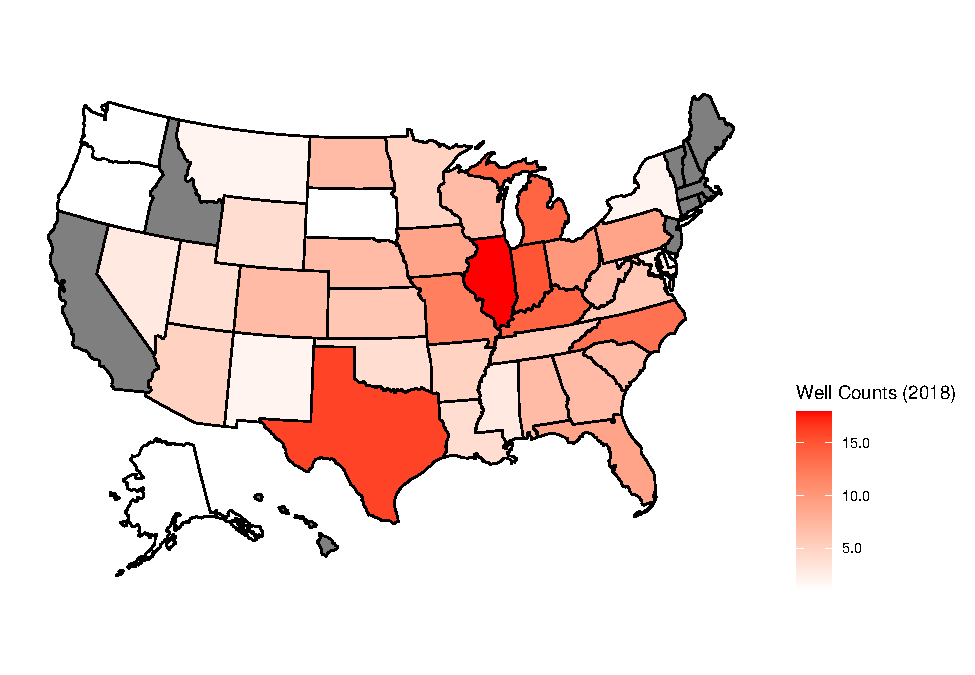
\includegraphics{Tony-Ni_StatThesis_files/figure-latex/usmap-1} 

}

\caption{Counts of Coal Sites in the United States (gray indicates no sites for that state).}\label{fig:usmap}
\end{figure}
\hypertarget{keldermans-top-10-sites}{%
\subsection{Kelderman's Top 10 Sites}\label{keldermans-top-10-sites}}

As stated previously, Kelderman et al. (2019) compiled a list of the top ten most contaminated sites across the U.S., following the EPA's health-based threshold for specific contaminants. We will briefly follow with a discussion on their methodology in determining these top ten most contaminated sites.

First, they calculated the average mean concentration for all contaminants in each well across all dates. To ensure that all observations used in this calculation were attributable to the coal site in question, there are several guidelines that were followed.

After these values are obtained, any wells with average downgradient concentrations lower than the highest average upgradient concentration for that specific contaminant and disposal area were removed. It is also important to note that since upgradient wells measure the quality of the water \emph{before} it passes through a coal site, they are also removed.

These two exclusion principles are followed to ensure that we did not use any wells that potentially had contamination from an external source, apart from the coal site. The remaining average mean concentrations of the contaminants in question for each site are then compared to the health-based thresholds set by the EPA, these thresholds can be viewed in Table \ref{tab:hbt}.
\begin{table}

\caption{\label{tab:hbt}Health-based thresholds set by EPA.}
\centering
\begin{tabular}[t]{lll}
\toprule
Contaminant & Exceedance Limit & Unit\\
\midrule
Antimony & 6 & ug/L\\
\addlinespace
Arsenic & 10 & ug/L\\
\addlinespace
Barium & 2 & mg/L\\
\addlinespace
Beryllium & 4 & ug/L\\
\addlinespace
Boron & 3 & mg/L\\
\addlinespace
Cadmium & 5 & ug/L\\
\addlinespace
Chromium & 100 & ug/L\\
\addlinespace
Cobalt & 6 & ug/L\\
\addlinespace
Fluoride & 4 & mg/L\\
\addlinespace
Lead & 15 & ug/L\\
\addlinespace
Lithium & 40 & ug/L\\
\addlinespace
Mercury & 2 & ug/L\\
\addlinespace
Molybdenum & 40 & ug/L\\
\addlinespace
Radium & 5 & pCi/L\\
\addlinespace
Selenium & 50 & ug/L\\
\addlinespace
Sulfate & 500 & mg/L\\
\addlinespace
Thallium & 2 & ug/L\\
\bottomrule
\end{tabular}
\end{table}
For each site, the wells with the highest average concentration of each contaminant were identified and compared to their respective health-based thresholds. A ratio is then calculated for each of these highest average contaminants to the health-based thresholds. These contaminant-specific ratios are then summed together in order to get a cumulative ``contamination score'' for each site. Contamination scores of a higher magnitude indicates more ``severe'' contamination, with the top ten highest contamination scores comprising the top ten most contaminated sites.

While the contamination scores are not explicitly published in Kelderman et al. (2019)'s report, the site names of the top ten most contaminated sites in the country according to their analysis which in descending order severity are as follows:
\begin{verbatim}
  1. San Miguel Plant,
  2. Allen Steam Station
  3. Jim Bridger Power Plant
  4. Naughton Power Plant
  5. New Castle Generating Station
  6. Allen Fossil Plant
  7. Brandywine Ash Management Facility
  8. Hunter Power Plant
  9. R.D. Morrow, Sr. Generating Station
  10. Ghent Generating Station
\end{verbatim}
We will follow their criterion(s) for determining if a well is contaminated, with the only difference being how we obtain the average concentrations of the contaminants in the wells. We will use our several left-censored estimation techniques to obtain mean estimates of the concentrations while accounting for the values below the limit of detection and see if our results significantly differ from the top ten list of most contaminated sites obtained by Kelderman et al. (2019). We will also have a baseline implementation of the methods described by Kelderman et al. (2019), without any attempts to account for the censored data. This implementation will serve as our control in which we will compare our left-censored estimation techniques towards.

\hypertarget{our-top-ten-most-contaminated-sites}{%
\subsection{(Our) Top Ten Most Contaminated Sites}\label{our-top-ten-most-contaminated-sites}}
\begin{table}

\caption{\label{tab:top10baseline}Top 10 most contaminated sites 
             for our baseline (control) implementation.}
\centering
\fontsize{11.5}{13.5}\selectfont
\begin{tabular}[t]{lr}
\toprule
Site & Composite Score\\
\midrule
San Miguel Plant & 940\\
\addlinespace
Allen Steam Station & 565\\
\addlinespace
New Castle Generating Station & 441\\
\addlinespace
Brandywine Ash Management Facility & 422\\
\addlinespace
R.D. Morrow, Sr. Generating Station & 402\\
\addlinespace
Allen Fossil Plant & 368\\
\addlinespace
Hunter Power Plant & 345\\
\addlinespace
Naughton Power Plant & 273\\
\addlinespace
Jim Bridger Power Plant & 266\\
\addlinespace
Sebree Generating Station & 266\\
\bottomrule
\end{tabular}
\end{table}
\begin{table}

\caption{\label{tab:top10substitution}Top 10 most contaminated sites 
             for our substitution method implementation.}
\centering
\fontsize{11.5}{13.5}\selectfont
\begin{tabular}[t]{lr}
\toprule
Site & Composite Score\\
\midrule
San Miguel Plant & 939\\
\addlinespace
Allen Steam Station & 565\\
\addlinespace
New Castle Generating Station & 441\\
\addlinespace
Brandywine Ash Management Facility & 419\\
\addlinespace
R.D. Morrow, Sr. Generating Station & 403\\
\addlinespace
Allen Fossil Plant & 367\\
\addlinespace
Hunter Power Plant & 345\\
\addlinespace
Naughton Power Plant & 272\\
\addlinespace
Jim Bridger Power Plant & 265\\
\addlinespace
Sebree Generating Station & 264\\
\bottomrule
\end{tabular}
\end{table}
\begin{table}

\caption{\label{tab:top10km}Top 10 most contaminated sites 
             for our KM method implementation.}
\centering
\fontsize{11.5}{13.5}\selectfont
\begin{tabular}[t]{lr}
\toprule
Site & Composite Score\\
\midrule
San Miguel Plant & 941\\
\addlinespace
Allen Steam Station & 565\\
\addlinespace
New Castle Generating Station & 441\\
\addlinespace
Brandywine Ash Management Facility & 422\\
\addlinespace
R.D. Morrow, Sr. Generating Station & 404\\
\addlinespace
Allen Fossil Plant & 368\\
\addlinespace
Ghent Generating Station & 363\\
\addlinespace
Hunter Power Plant & 345\\
\addlinespace
Naughton Power Plant & 274\\
\addlinespace
Jim Bridger Power Plant & 265\\
\bottomrule
\end{tabular}
\end{table}
The results from our baseline implementation which calculates mean estimates without any attempt to account for censoring, obtains the top ten sites presented in Table \ref{tab:top10baseline}. When comparing this to the original substitution method using 1/2(LOD) implemented by Kelderman et al. (2019), 9 out of the 10 sites are shared, with the only major difference being the order in which the sites are presented. As the composite scores of the sites were not originally published in Kelderman et al. (2019)'s report, we are unable to delve into more of the specifics regarding the magnitude of difference between the two implementations. As such, we found it prudent to perform their analysis using the substitution method, the results of which are presented in Table \ref{tab:top10substitution}.

Something unexpected to note is that although we followed the procedures outlined by Kelderman et al. (2019) in their implementation of the substitution method, our top ten sites presented in Table \ref{tab:top10km} somewhat differ from theirs. Reproducible code was not provided in their report and attempts to completely reproduce their top ten list would not be conducive to the goal of this report. As such, from now on, we will proceed with the analysis with \emph{our} top ten list produced by the substitution method as the norm, for the sake of comparability with our other methods.

It is also important to note that the MLE method and the ROS method are absent from this case-study. It can be recalled that in our previous discussion regarding the MLE method, we discussed noted a limitation of the MLE method being how it can obtain overinflated estimates when the data is highly skewed. In our attempt to use the MLE method, we found that the estimates we obtained did not provide very useful information. To exemplify this, we had one well with an abnormally large concentration, a sign that it was most likely contaminated, and hundreds of smaller wells in which the concentration is 0. The MLE method gave us mean estimates nearing infinity, which threw our analysis into disarray. As such, we refrained from utilizing the MLE method in this specific case study.

The ROS method was absent for a similar reason, but with the limitations more-so being on the capabilities of the method itself. As we discussed previously, the ROS method can only be used in settings when more than half the data is uncensored. Unfortunately with our data, censoring far exceeds 50\%, and as such, the ROS method is unable to be implemented (Environmental Protection Agency, 2009).

The top ten sites obtained using our substitution implementation are the same sites as the ones obtained from our baseline implementation, with the same ordering but slight differences in the composite scores. With our KM method, the Ghent Generating Station replaces the Sebree Generating Station as one of the top ten most contaminated sites, with some slight differences in the ordering of the sites in the latter half of the list.

It is not a surprise that our left-censoring mean estimation techniques did not provide much of a different result than what we obtained with our baseline implementation. Left-censoring techniques are not as useful with this case-study, where we are focused on finding the extremities of the dataset, i.e.~wells with the highest concentration of contaminants. If the research question was instead, identifying wells that were potentially contaminated, the distinction between the results obtained by these methods would be more visible. Kelderman et al. (2019)'s implementation of the substitution method as a way to account for left-censoring is justifiable due to its ease of implementation and the results we just discussed, regarding the lack of differences in top ten sites when comparing all three implementations we used.

\hypertarget{conclusion}{%
\chapter{Conclusion}\label{conclusion}}

{[}write a few paragraphs to wrap up entire thesis{]}

\appendix

\hypertarget{main-appendix}{%
\chapter{Main Appendix}\label{main-appendix}}

This first appendix includes all of the R chunks of code that were hidden throughout the document (using the \texttt{include\ =\ FALSE} chunk tag) to help with readibility and/or setup.

\hypertarget{in-the-main-file-refref-labels}{%
\section{In the main file \ref{ref-labels}:}\label{in-the-main-file-refref-labels}}

\hypertarget{in-chapter-refref-labels}{%
\section{In Chapter \ref{ref-labels}:}\label{in-chapter-refref-labels}}

\hypertarget{in-chapter-3}{%
\section{In Chapter 3:}\label{in-chapter-3}}
\begin{Shaded}
\begin{Highlighting}[]
\CommentTok{\#breaking apart into different datasets for each region}
\NormalTok{northeast }\OtherTok{\textless{}{-}}\NormalTok{ import\_df }\SpecialCharTok{\%\textgreater{}\%}
  \FunctionTok{filter}\NormalTok{(state }\SpecialCharTok{\%in\%} \FunctionTok{c}\NormalTok{(}\StringTok{"ME"}\NormalTok{, }\StringTok{"NH"}\NormalTok{, }\StringTok{"VT"}\NormalTok{, }\StringTok{"NY"}\NormalTok{, }\StringTok{"PA"}\NormalTok{, }\StringTok{"NJ"}\NormalTok{, }\StringTok{"MD"}\NormalTok{, }
                      \StringTok{"MA"}\NormalTok{, }\StringTok{"DE"}\NormalTok{, }\StringTok{"RI"}\NormalTok{, }\StringTok{"CT"}\NormalTok{)) }\SpecialCharTok{\%\textgreater{}\%}
  \FunctionTok{mutate}\NormalTok{(}\AttributeTok{region =} \StringTok{"northeast"}\NormalTok{)}

\NormalTok{midwest }\OtherTok{\textless{}{-}}\NormalTok{ import\_df }\SpecialCharTok{\%\textgreater{}\%}
  \FunctionTok{filter}\NormalTok{(state }\SpecialCharTok{\%in\%} \FunctionTok{c}\NormalTok{(}\StringTok{"OH"}\NormalTok{, }\StringTok{"IN"}\NormalTok{, }\StringTok{"MI"}\NormalTok{, }\StringTok{"IL"}\NormalTok{, }\StringTok{"WI"}\NormalTok{, }\StringTok{"MN"}\NormalTok{, }\StringTok{"IA"}\NormalTok{, }
                      \StringTok{"MO"}\NormalTok{, }\StringTok{"ND"}\NormalTok{, }\StringTok{"SD"}\NormalTok{, }\StringTok{"NE"}\NormalTok{, }\StringTok{"KS"}\NormalTok{))}\SpecialCharTok{\%\textgreater{}\%}
  \FunctionTok{mutate}\NormalTok{(}\AttributeTok{region =} \StringTok{"midwest"}\NormalTok{)}

\NormalTok{west }\OtherTok{\textless{}{-}}\NormalTok{ import\_df }\SpecialCharTok{\%\textgreater{}\%}
  \FunctionTok{filter}\NormalTok{(state }\SpecialCharTok{\%in\%} \FunctionTok{c}\NormalTok{(}\StringTok{"WA"}\NormalTok{, }\StringTok{"MT"}\NormalTok{, }\StringTok{"OR"}\NormalTok{, }\StringTok{"ID"}\NormalTok{, }\StringTok{"WY"}\NormalTok{, }\StringTok{"CA"}\NormalTok{, }\StringTok{"NV"}\NormalTok{, }
                      \StringTok{"UT"}\NormalTok{, }\StringTok{"CO"}\NormalTok{, }\StringTok{"AZ"}\NormalTok{, }\StringTok{"NM"}\NormalTok{, }\StringTok{"AK"}\NormalTok{, }\StringTok{"HI"}\NormalTok{)) }\SpecialCharTok{\%\textgreater{}\%}
  \FunctionTok{mutate}\NormalTok{(}\AttributeTok{region =} \StringTok{"west"}\NormalTok{)}

\NormalTok{south }\OtherTok{\textless{}{-}}\NormalTok{ import\_df }\SpecialCharTok{\%\textgreater{}\%}
  \FunctionTok{filter}\NormalTok{(state }\SpecialCharTok{\%in\%} \FunctionTok{c}\NormalTok{(}\StringTok{"WV"}\NormalTok{, }\StringTok{"VA"}\NormalTok{, }\StringTok{"KY"}\NormalTok{, }\StringTok{"TN"}\NormalTok{, }\StringTok{"NC"}\NormalTok{, }\StringTok{"SC"}\NormalTok{, }\StringTok{"GA"}\NormalTok{, }
                      \StringTok{"FL"}\NormalTok{, }\StringTok{"MS"}\NormalTok{, }\StringTok{"AL"}\NormalTok{, }\StringTok{"LA"}\NormalTok{, }\StringTok{"AR"}\NormalTok{, }\StringTok{"OK"}\NormalTok{, }\StringTok{"TX"}\NormalTok{, }\StringTok{"PR"}\NormalTok{)) }\SpecialCharTok{\%\textgreater{}\%}
  \FunctionTok{mutate}\NormalTok{(}\AttributeTok{region =} \StringTok{"south"}\NormalTok{)}

\CommentTok{\#rejoin them back together for future ref. if needed}
\NormalTok{full }\OtherTok{\textless{}{-}} \FunctionTok{list}\NormalTok{(northeast, midwest, west, south) }\SpecialCharTok{\%\textgreater{}\%} 
  \FunctionTok{reduce}\NormalTok{(full\_join) }\SpecialCharTok{\%\textgreater{}\%}
  \FunctionTok{select}\NormalTok{(}\SpecialCharTok{{-}}\FunctionTok{c}\NormalTok{(}\StringTok{"qualifier"}\NormalTok{, }\StringTok{"link"}\NormalTok{))}

\CommentTok{\#getting \# of sites in each state}

\NormalTok{midwest\_n }\OtherTok{\textless{}{-}}\NormalTok{ midwest }\SpecialCharTok{\%\textgreater{}\%}
  \FunctionTok{group\_by}\NormalTok{(state) }\SpecialCharTok{\%\textgreater{}\%}
  \FunctionTok{distinct}\NormalTok{(site) }\SpecialCharTok{\%\textgreater{}\%}
  \FunctionTok{summarize}\NormalTok{(}\AttributeTok{n =} \FunctionTok{n}\NormalTok{())}

\NormalTok{northeast\_n }\OtherTok{\textless{}{-}}\NormalTok{ northeast }\SpecialCharTok{\%\textgreater{}\%}
  \FunctionTok{group\_by}\NormalTok{(state) }\SpecialCharTok{\%\textgreater{}\%}
  \FunctionTok{distinct}\NormalTok{(site) }\SpecialCharTok{\%\textgreater{}\%}
  \FunctionTok{summarize}\NormalTok{(}\AttributeTok{n =} \FunctionTok{n}\NormalTok{())}

\NormalTok{south\_n }\OtherTok{\textless{}{-}}\NormalTok{ south }\SpecialCharTok{\%\textgreater{}\%}
  \FunctionTok{group\_by}\NormalTok{(state) }\SpecialCharTok{\%\textgreater{}\%}
  \FunctionTok{distinct}\NormalTok{(site) }\SpecialCharTok{\%\textgreater{}\%}
  \FunctionTok{summarize}\NormalTok{(}\AttributeTok{n =} \FunctionTok{n}\NormalTok{())}

\NormalTok{west\_n }\OtherTok{\textless{}{-}}\NormalTok{ west }\SpecialCharTok{\%\textgreater{}\%}
  \FunctionTok{group\_by}\NormalTok{(state) }\SpecialCharTok{\%\textgreater{}\%}
  \FunctionTok{distinct}\NormalTok{(site) }\SpecialCharTok{\%\textgreater{}\%}
  \FunctionTok{summarize}\NormalTok{(}\AttributeTok{n =} \FunctionTok{n}\NormalTok{())}

\NormalTok{states\_n }\OtherTok{\textless{}{-}} \FunctionTok{rbind}\NormalTok{(midwest\_n, northeast\_n, south\_n, west\_n)}

\NormalTok{state\_name }\OtherTok{\textless{}{-}}\NormalTok{ state.name}
\NormalTok{state\_abb }\OtherTok{\textless{}{-}}\NormalTok{ state.abb}
\NormalTok{states\_map }\OtherTok{\textless{}{-}} \FunctionTok{map\_data}\NormalTok{(}\StringTok{"state"}\NormalTok{)}
\end{Highlighting}
\end{Shaded}
\hypertarget{simulation-and-case-study-appendix}{%
\chapter{Simulation and Case Study Appendix}\label{simulation-and-case-study-appendix}}

The second appendix, Appendix B, contains all necessary code required to run the simulation study and for our case study.

\hypertarget{simulation-study}{%
\section{Simulation Study}\label{simulation-study}}

\hypertarget{libraries}{%
\subsection{Libraries}\label{libraries}}
\begin{Shaded}
\begin{Highlighting}[]
\FunctionTok{library}\NormalTok{(tidyverse)}
\FunctionTok{library}\NormalTok{(Metrics) }\CommentTok{\#package to help calculate mse}
\FunctionTok{library}\NormalTok{(NADA) }\CommentTok{\#package with implementation of many methods}
\FunctionTok{library}\NormalTok{(survival)}
\FunctionTok{library}\NormalTok{(kableExtra)}
\end{Highlighting}
\end{Shaded}
\hypertarget{generating-data}{%
\subsection{Generating Data}\label{generating-data}}
\begin{Shaded}
\begin{Highlighting}[]
\CommentTok{\#function will generate a vector of numbers from the lognormal }
\CommentTok{\#distribution and censor them at the given rate}
\CommentTok{\#function will take in arguments for 1) samplesize, 2) logmean, 3)logsd}
\CommentTok{\#4) censoring rate}

\NormalTok{generateLN }\OtherTok{\textless{}{-}} \ControlFlowTok{function}\NormalTok{(sampsize, m, s, censrate)\{}
\NormalTok{  true.value }\OtherTok{\textless{}{-}} \FunctionTok{rlnorm}\NormalTok{(sampsize, }
               \AttributeTok{meanlog=}\FunctionTok{log}\NormalTok{(m}\SpecialCharTok{\^{}}\DecValTok{2} \SpecialCharTok{/} \FunctionTok{sqrt}\NormalTok{(s}\SpecialCharTok{\^{}}\DecValTok{2} \SpecialCharTok{+}\NormalTok{ m}\SpecialCharTok{\^{}}\DecValTok{2}\NormalTok{)),}
               \AttributeTok{sdlog=}\FunctionTok{sqrt}\NormalTok{(}\FunctionTok{log}\NormalTok{(}\DecValTok{1} \SpecialCharTok{+}\NormalTok{ (s}\SpecialCharTok{\^{}}\DecValTok{2} \SpecialCharTok{/}\NormalTok{ m}\SpecialCharTok{\^{}}\DecValTok{2}\NormalTok{))))}
  
\NormalTok{  uncensored\_df }\OtherTok{\textless{}{-}} \FunctionTok{as.data.frame}\NormalTok{(true.value) }\SpecialCharTok{\%\textgreater{}\%}
    \FunctionTok{arrange}\NormalTok{(true.value)}
  
\NormalTok{  censored\_df }\OtherTok{\textless{}{-}}\NormalTok{ uncensored\_df }\SpecialCharTok{\%\textgreater{}\%} \CommentTok{\#take the head(\%) of data to be censored}
    \FunctionTok{slice\_head}\NormalTok{(}\AttributeTok{n=}\FunctionTok{nrow}\NormalTok{(uncensored\_df)}\SpecialCharTok{*}\NormalTok{censrate) }\SpecialCharTok{\%\textgreater{}\%}
    \FunctionTok{mutate}\NormalTok{(}\AttributeTok{censored =} \ConstantTok{TRUE}\NormalTok{)}
  
  \CommentTok{\#full join original df and sliced df}
\NormalTok{  return\_df }\OtherTok{\textless{}{-}} \FunctionTok{full\_join}\NormalTok{(uncensored\_df, censored\_df, }\AttributeTok{by =} \StringTok{"true.value"}\NormalTok{)}

  \CommentTok{\#replace NAs with FALSE}
\NormalTok{  return\_df}\SpecialCharTok{$}\NormalTok{censored }\OtherTok{\textless{}{-}} \FunctionTok{replace\_na}\NormalTok{(return\_df}\SpecialCharTok{$}\NormalTok{censored, }\AttributeTok{replace =} \ConstantTok{FALSE}\NormalTok{)}
  
  \FunctionTok{return}\NormalTok{(return\_df)}
\NormalTok{\}}
\CommentTok{\#function will generate a vector of numbers from the exponential }
\CommentTok{\#distribution and censor them at the given rate}
\CommentTok{\#function will take in arguments for 1) samplesize, 2) rate,}
\CommentTok{\#3) censoring rate}

\NormalTok{generateEXP }\OtherTok{\textless{}{-}} \ControlFlowTok{function}\NormalTok{(sampsize, r, censrate)\{}
\NormalTok{  true.value }\OtherTok{\textless{}{-}} \FunctionTok{rexp}\NormalTok{(sampsize, }\AttributeTok{rate =}\NormalTok{ r)}
  
\NormalTok{  uncensored\_df }\OtherTok{\textless{}{-}} \FunctionTok{as.data.frame}\NormalTok{(true.value) }\SpecialCharTok{\%\textgreater{}\%}
    \FunctionTok{arrange}\NormalTok{(true.value)}
  
\NormalTok{  censored\_df }\OtherTok{\textless{}{-}}\NormalTok{ uncensored\_df }\SpecialCharTok{\%\textgreater{}\%} \CommentTok{\#take the head(\%) of data to be censored}
    \FunctionTok{slice\_head}\NormalTok{(}\AttributeTok{n=}\FunctionTok{nrow}\NormalTok{(uncensored\_df)}\SpecialCharTok{*}\NormalTok{censrate) }\SpecialCharTok{\%\textgreater{}\%}
    \FunctionTok{mutate}\NormalTok{(}\AttributeTok{censored =} \ConstantTok{TRUE}\NormalTok{)}
  
  \CommentTok{\#full join original df and sliced df}
\NormalTok{  return\_df }\OtherTok{\textless{}{-}} \FunctionTok{full\_join}\NormalTok{(uncensored\_df, censored\_df, }\AttributeTok{by =} \StringTok{"true.value"}\NormalTok{)}

  \CommentTok{\#replace NAs with FALSE}
\NormalTok{  return\_df}\SpecialCharTok{$}\NormalTok{censored }\OtherTok{\textless{}{-}} \FunctionTok{replace\_na}\NormalTok{(return\_df}\SpecialCharTok{$}\NormalTok{censored, }\AttributeTok{replace =} \ConstantTok{FALSE}\NormalTok{)}
  
  \FunctionTok{return}\NormalTok{(return\_df)}
\NormalTok{\}}
\CommentTok{\#function will generate a vector of numbers from the Weibull}
\CommentTok{\#distribution and censor them at the given rate}
\CommentTok{\#function will take in arguments for 1) samplesize, 2) rate,}
\CommentTok{\#3) censoring rate}

\NormalTok{generateW }\OtherTok{\textless{}{-}} \ControlFlowTok{function}\NormalTok{(sampsize, sh, sc, censrate)\{}
\NormalTok{  true.value }\OtherTok{\textless{}{-}} \FunctionTok{rweibull}\NormalTok{(sampsize, }\AttributeTok{shape =}\NormalTok{ sh, }\AttributeTok{scale =}\NormalTok{ sc)}
  
\NormalTok{  uncensored\_df }\OtherTok{\textless{}{-}} \FunctionTok{as.data.frame}\NormalTok{(true.value) }\SpecialCharTok{\%\textgreater{}\%}
    \FunctionTok{arrange}\NormalTok{(true.value)}
  
\NormalTok{  censored\_df }\OtherTok{\textless{}{-}}\NormalTok{ uncensored\_df }\SpecialCharTok{\%\textgreater{}\%} \CommentTok{\#take the head(\%) of data to be censored}
    \FunctionTok{slice\_head}\NormalTok{(}\AttributeTok{n=}\FunctionTok{nrow}\NormalTok{(uncensored\_df)}\SpecialCharTok{*}\NormalTok{censrate) }\SpecialCharTok{\%\textgreater{}\%}
    \FunctionTok{mutate}\NormalTok{(}\AttributeTok{censored =} \ConstantTok{TRUE}\NormalTok{)}
  
  \CommentTok{\#full join original df and sliced df}
\NormalTok{  return\_df }\OtherTok{\textless{}{-}} \FunctionTok{full\_join}\NormalTok{(uncensored\_df, censored\_df, }\AttributeTok{by =} \StringTok{"true.value"}\NormalTok{)}

  \CommentTok{\#replace NAs with FALSE}
\NormalTok{  return\_df}\SpecialCharTok{$}\NormalTok{censored }\OtherTok{\textless{}{-}} \FunctionTok{replace\_na}\NormalTok{(return\_df}\SpecialCharTok{$}\NormalTok{censored, }\AttributeTok{replace =} \ConstantTok{FALSE}\NormalTok{)}
  
  \FunctionTok{return}\NormalTok{(return\_df)}
\NormalTok{\}}
\end{Highlighting}
\end{Shaded}
\hypertarget{setup}{%
\subsection{Setup}\label{setup}}
\begin{Shaded}
\begin{Highlighting}[]
\NormalTok{iterations }\OtherTok{\textless{}{-}} \DecValTok{1000} \CommentTok{\#number of iterations}
\NormalTok{censvalues }\OtherTok{\textless{}{-}} \FunctionTok{c}\NormalTok{(}\FloatTok{0.10}\NormalTok{, }\FloatTok{0.30}\NormalTok{, }\FloatTok{0.50}\NormalTok{)}
\NormalTok{sampsizes }\OtherTok{\textless{}{-}} \FunctionTok{c}\NormalTok{(}\DecValTok{10}\NormalTok{, }\DecValTok{100}\NormalTok{, }\DecValTok{1000}\NormalTok{)}

\NormalTok{df.tall }\OtherTok{\textless{}{-}} \FunctionTok{data.frame}\NormalTok{(}\AttributeTok{prop\_cens =} \FunctionTok{numeric}\NormalTok{(),}
                      \AttributeTok{samplesize =} \FunctionTok{numeric}\NormalTok{(),}
                      \AttributeTok{iteration =} \FunctionTok{numeric}\NormalTok{(),}
                      \AttributeTok{method =} \FunctionTok{character}\NormalTok{(),}
                      \AttributeTok{true\_mean =} \FunctionTok{numeric}\NormalTok{(),}
                      \AttributeTok{mean\_complete =} \FunctionTok{numeric}\NormalTok{(),}
                      \AttributeTok{mean\_method =} \FunctionTok{numeric}\NormalTok{(),}
                      \AttributeTok{true\_sd =} \FunctionTok{numeric}\NormalTok{(),}
                      \AttributeTok{SE\_complete =} \FunctionTok{numeric}\NormalTok{(),}
                      \AttributeTok{SE\_method =} \FunctionTok{numeric}\NormalTok{())}
\end{Highlighting}
\end{Shaded}
\hypertarget{lognormal}{%
\subsection{Lognormal}\label{lognormal}}
\begin{Shaded}
\begin{Highlighting}[]
\CommentTok{\#LOGNORMAL}
\FunctionTok{options}\NormalTok{(}\AttributeTok{scipen=}\DecValTok{999}\NormalTok{) }\CommentTok{\#prevent scientific notation}
\FunctionTok{set.seed}\NormalTok{(}\DecValTok{7271999}\NormalTok{)}

\ControlFlowTok{for}\NormalTok{(i }\ControlFlowTok{in}\NormalTok{ censvalues)\{}
  \ControlFlowTok{for}\NormalTok{(j }\ControlFlowTok{in}\NormalTok{ sampsizes)\{}
    \ControlFlowTok{for}\NormalTok{(k }\ControlFlowTok{in} \DecValTok{1}\SpecialCharTok{:}\NormalTok{iterations)\{}
\NormalTok{      m }\OtherTok{\textless{}{-}} \DecValTok{1}
\NormalTok{      s }\OtherTok{\textless{}{-}} \FloatTok{0.5}
\NormalTok{      df }\OtherTok{\textless{}{-}} \FunctionTok{generateLN}\NormalTok{(}\AttributeTok{sampsize =}\NormalTok{ j, }\AttributeTok{m =} \DecValTok{1}\NormalTok{, }\AttributeTok{s =} \FloatTok{0.5}\NormalTok{, }\AttributeTok{censrate =}\NormalTok{ i)}
      
      \CommentTok{\#substitution}
      \CommentTok{\#define LOD to be smallest, uncensored value}
\NormalTok{      LOD }\OtherTok{\textless{}{-}} \FunctionTok{min}\NormalTok{(df}\SpecialCharTok{$}\NormalTok{true.value[df}\SpecialCharTok{$}\NormalTok{censored }\SpecialCharTok{==} \ConstantTok{FALSE}\NormalTok{]) }
\NormalTok{      df }\OtherTok{\textless{}{-}}\NormalTok{ df }\SpecialCharTok{\%\textgreater{}\%}
        \FunctionTok{mutate}\NormalTok{(}\AttributeTok{impSubValue =} \FunctionTok{if\_else}\NormalTok{(censored }\SpecialCharTok{==} \ConstantTok{TRUE}\NormalTok{, LOD}\SpecialCharTok{/}\DecValTok{2}\NormalTok{, true.value))}
      
\NormalTok{      df.tall }\OtherTok{\textless{}{-}}\NormalTok{ df.tall }\SpecialCharTok{\%\textgreater{}\%}
        \FunctionTok{add\_row}\NormalTok{(}\AttributeTok{prop\_cens =}\NormalTok{ i,}
                \AttributeTok{samplesize =}\NormalTok{ j,}
                \AttributeTok{iteration =}\NormalTok{ k,}
                \AttributeTok{method =} \StringTok{"substitution"}\NormalTok{,}
                \AttributeTok{true\_mean =}\NormalTok{ m,}
                \AttributeTok{mean\_complete =} \FunctionTok{mean}\NormalTok{(df}\SpecialCharTok{$}\NormalTok{true.value),}
                \AttributeTok{mean\_method =} \FunctionTok{mean}\NormalTok{(df}\SpecialCharTok{$}\NormalTok{impSubValue),}
                \AttributeTok{true\_sd =}\NormalTok{ s,}
                \AttributeTok{SE\_complete =} 
                  \FunctionTok{sd}\NormalTok{(df}\SpecialCharTok{$}\NormalTok{true.value)}\SpecialCharTok{/}\FunctionTok{sqrt}\NormalTok{((}\FunctionTok{length}\NormalTok{(df}\SpecialCharTok{$}\NormalTok{true.value))),}
                \AttributeTok{SE\_method =} 
                  \FunctionTok{sd}\NormalTok{(df}\SpecialCharTok{$}\NormalTok{impSubValue)}\SpecialCharTok{/}\FunctionTok{sqrt}\NormalTok{((}\FunctionTok{length}\NormalTok{(df}\SpecialCharTok{$}\NormalTok{impSubValue))))}
      
      \CommentTok{\#mle}
\NormalTok{      mle\_res }\OtherTok{=} \FunctionTok{cenmle}\NormalTok{(df}\SpecialCharTok{$}\NormalTok{true.value, df}\SpecialCharTok{$}\NormalTok{censored)}
      
\NormalTok{      df.tall }\OtherTok{\textless{}{-}}\NormalTok{ df.tall }\SpecialCharTok{\%\textgreater{}\%}
        \FunctionTok{add\_row}\NormalTok{(}\AttributeTok{prop\_cens =}\NormalTok{ i,}
                \AttributeTok{samplesize =}\NormalTok{ j,}
                \AttributeTok{iteration =}\NormalTok{ k,}
                \AttributeTok{method =} \StringTok{"mle"}\NormalTok{,}
                \AttributeTok{true\_mean =}\NormalTok{ m,}
                \AttributeTok{mean\_complete =} \FunctionTok{mean}\NormalTok{(df}\SpecialCharTok{$}\NormalTok{true.value),}
                \AttributeTok{mean\_method =} \FunctionTok{mean}\NormalTok{(mle\_res)[}\DecValTok{1}\NormalTok{],}
                \AttributeTok{true\_sd =}\NormalTok{ s,}
                \AttributeTok{SE\_complete =} 
                  \FunctionTok{sd}\NormalTok{(df}\SpecialCharTok{$}\NormalTok{true.value)}\SpecialCharTok{/}\FunctionTok{sqrt}\NormalTok{((}\FunctionTok{length}\NormalTok{(df}\SpecialCharTok{$}\NormalTok{true.value))),}
                \AttributeTok{SE\_method =} \FunctionTok{mean}\NormalTok{(mle\_res)[}\DecValTok{2}\NormalTok{])}
      
      \CommentTok{\#km}
\NormalTok{      km\_res }\OtherTok{=} \FunctionTok{cenfit}\NormalTok{(df}\SpecialCharTok{$}\NormalTok{true.value, df}\SpecialCharTok{$}\NormalTok{censored)}
      
\NormalTok{      df.tall }\OtherTok{\textless{}{-}}\NormalTok{ df.tall }\SpecialCharTok{\%\textgreater{}\%}
        \FunctionTok{add\_row}\NormalTok{(}\AttributeTok{prop\_cens =}\NormalTok{ i,}
                \AttributeTok{samplesize =}\NormalTok{ j,}
                \AttributeTok{iteration =}\NormalTok{ k,}
                \AttributeTok{method =} \StringTok{"km"}\NormalTok{,}
                \AttributeTok{true\_mean =}\NormalTok{ m,}
                \AttributeTok{mean\_complete =} \FunctionTok{mean}\NormalTok{(df}\SpecialCharTok{$}\NormalTok{true.value),}
                \AttributeTok{mean\_method =} \FunctionTok{mean}\NormalTok{(km\_res)[[}\DecValTok{1}\NormalTok{]],}
                \AttributeTok{true\_sd =}\NormalTok{ s,}
                \AttributeTok{SE\_complete =} 
                  \FunctionTok{sd}\NormalTok{(df}\SpecialCharTok{$}\NormalTok{true.value)}\SpecialCharTok{/}\FunctionTok{sqrt}\NormalTok{((}\FunctionTok{length}\NormalTok{(df}\SpecialCharTok{$}\NormalTok{true.value))),}
                \AttributeTok{SE\_method =} \FunctionTok{mean}\NormalTok{(km\_res)[[}\DecValTok{2}\NormalTok{]])}
      
      \CommentTok{\#ros}
\NormalTok{      ros\_res }\OtherTok{=} \FunctionTok{ros}\NormalTok{(df}\SpecialCharTok{$}\NormalTok{true.value, df}\SpecialCharTok{$}\NormalTok{censored)}
      
\NormalTok{      df.tall }\OtherTok{\textless{}{-}}\NormalTok{ df.tall }\SpecialCharTok{\%\textgreater{}\%}
        \FunctionTok{add\_row}\NormalTok{(}\AttributeTok{prop\_cens =}\NormalTok{ i,}
                \AttributeTok{samplesize =}\NormalTok{ j,}
                \AttributeTok{iteration =}\NormalTok{ k,}
                \AttributeTok{method =} \StringTok{"ros"}\NormalTok{,}
                \AttributeTok{true\_mean =}\NormalTok{ m,}
                \AttributeTok{mean\_complete =} \FunctionTok{mean}\NormalTok{(df}\SpecialCharTok{$}\NormalTok{true.value),}
                \AttributeTok{mean\_method =} \FunctionTok{mean}\NormalTok{(ros\_res),}
                \AttributeTok{true\_sd =}\NormalTok{ s,}
                \AttributeTok{SE\_complete =} 
                  \FunctionTok{sd}\NormalTok{(df}\SpecialCharTok{$}\NormalTok{true.value)}\SpecialCharTok{/}\FunctionTok{sqrt}\NormalTok{((}\FunctionTok{length}\NormalTok{(df}\SpecialCharTok{$}\NormalTok{true.value))),}
                \AttributeTok{SE\_method =} 
                  \FunctionTok{sd}\NormalTok{(ros\_res)}\SpecialCharTok{/}\FunctionTok{sqrt}\NormalTok{((}\FunctionTok{length}\NormalTok{(df}\SpecialCharTok{$}\NormalTok{true.value))))}
\NormalTok{    \}}
    \CommentTok{\#end of \# iterations}
\NormalTok{  \}}
\NormalTok{\}}

\CommentTok{\#aggregating performance criteria}

\NormalTok{df.ln }\OtherTok{\textless{}{-}}\NormalTok{ df.tall }\SpecialCharTok{\%\textgreater{}\%}
  \FunctionTok{group\_by}\NormalTok{(prop\_cens, samplesize, method) }\SpecialCharTok{\%\textgreater{}\%}
  \FunctionTok{summarize}\NormalTok{(}\AttributeTok{Avg\_Mean =} \FunctionTok{mean}\NormalTok{(mean\_method),}
            \AttributeTok{Bias =}\NormalTok{ (}\FunctionTok{mean}\NormalTok{(mean\_method) }\SpecialCharTok{{-}}\NormalTok{ true\_mean),}
            \AttributeTok{Variance =} \FunctionTok{var}\NormalTok{(mean\_method),}
            \AttributeTok{MSE =} \FunctionTok{mse}\NormalTok{(true\_mean, mean\_method) }
\NormalTok{            ) }\SpecialCharTok{\%\textgreater{}\%}
  \FunctionTok{distinct}\NormalTok{() }\SpecialCharTok{\%\textgreater{}\%}
  \FunctionTok{ungroup}\NormalTok{()}
\end{Highlighting}
\end{Shaded}
\hypertarget{exponential}{%
\subsection{Exponential}\label{exponential}}
\begin{Shaded}
\begin{Highlighting}[]
\CommentTok{\#EXPONENTIAL}
\FunctionTok{options}\NormalTok{(}\AttributeTok{scipen=}\DecValTok{999}\NormalTok{) }\CommentTok{\#prevent scientific notation}
\FunctionTok{set.seed}\NormalTok{(}\DecValTok{7271999}\NormalTok{)}

\ControlFlowTok{for}\NormalTok{(i }\ControlFlowTok{in}\NormalTok{ censvalues)\{}
  \ControlFlowTok{for}\NormalTok{(j }\ControlFlowTok{in}\NormalTok{ sampsizes)\{}
    \ControlFlowTok{for}\NormalTok{(k }\ControlFlowTok{in} \DecValTok{1}\SpecialCharTok{:}\NormalTok{iterations)\{}
\NormalTok{      r }\OtherTok{=} \DecValTok{1}
\NormalTok{      df }\OtherTok{\textless{}{-}} \FunctionTok{generateEXP}\NormalTok{(}\AttributeTok{sampsize =}\NormalTok{ j, }\AttributeTok{r =}\NormalTok{ r, }\AttributeTok{censrate =}\NormalTok{ i)}

      \CommentTok{\#substitution}
      \CommentTok{\#define LOD to be smallest, uncensored value}
\NormalTok{      LOD }\OtherTok{\textless{}{-}} \FunctionTok{min}\NormalTok{(df}\SpecialCharTok{$}\NormalTok{true.value[df}\SpecialCharTok{$}\NormalTok{censored }\SpecialCharTok{==} \ConstantTok{FALSE}\NormalTok{]) }
\NormalTok{      df }\OtherTok{\textless{}{-}}\NormalTok{ df }\SpecialCharTok{\%\textgreater{}\%}
        \FunctionTok{mutate}\NormalTok{(}\AttributeTok{impSubValue =} \FunctionTok{if\_else}\NormalTok{(censored }\SpecialCharTok{==} \ConstantTok{TRUE}\NormalTok{, LOD}\SpecialCharTok{/}\DecValTok{2}\NormalTok{, true.value))}
      
\NormalTok{      df.tall }\OtherTok{\textless{}{-}}\NormalTok{ df.tall }\SpecialCharTok{\%\textgreater{}\%}
        \FunctionTok{add\_row}\NormalTok{(}\AttributeTok{prop\_cens =}\NormalTok{ i,}
                \AttributeTok{samplesize =}\NormalTok{ j,}
                \AttributeTok{iteration =}\NormalTok{ k,}
                \AttributeTok{method =} \StringTok{"substitution"}\NormalTok{,}
                \AttributeTok{true\_mean =} \DecValTok{1}\SpecialCharTok{/}\NormalTok{r,}
                \AttributeTok{mean\_complete =} \FunctionTok{mean}\NormalTok{(df}\SpecialCharTok{$}\NormalTok{true.value),}
                \AttributeTok{mean\_method =} \FunctionTok{mean}\NormalTok{(df}\SpecialCharTok{$}\NormalTok{impSubValue),}
                \AttributeTok{true\_sd =} \DecValTok{1}\SpecialCharTok{/}\NormalTok{r,}
                \AttributeTok{SE\_complete =} 
                  \FunctionTok{sd}\NormalTok{(df}\SpecialCharTok{$}\NormalTok{true.value)}\SpecialCharTok{/}\FunctionTok{sqrt}\NormalTok{((}\FunctionTok{length}\NormalTok{(df}\SpecialCharTok{$}\NormalTok{true.value))),}
                \AttributeTok{SE\_method =} 
                  \FunctionTok{sd}\NormalTok{(df}\SpecialCharTok{$}\NormalTok{impSubValue)}\SpecialCharTok{/}\FunctionTok{sqrt}\NormalTok{((}\FunctionTok{length}\NormalTok{(df}\SpecialCharTok{$}\NormalTok{impSubValue))))}
      
      \CommentTok{\#mle}
      \CommentTok{\# mle\_res = cenmle(df$true.value, df$censored)}
      \CommentTok{\# }
      \CommentTok{\# df.tall \textless{}{-} df.tall \%\textgreater{}\%}
      \CommentTok{\#   add\_row(prop\_cens = i,}
      \CommentTok{\#           samplesize = j,}
      \CommentTok{\#           iteration = k,}
      \CommentTok{\#           method = "mle",}
      \CommentTok{\#           true\_mean = 1/r,}
      \CommentTok{\#           mean\_complete = mean(df$true.value),}
      \CommentTok{\#           mean\_method = mean(mle\_res)[1],}
      \CommentTok{\#           true\_sd = 1/r,}
      \CommentTok{\#           SE\_complete = }
      \CommentTok{\#             sd(df$true.value)/sqrt((length(df$true.value))),}
      \CommentTok{\#           SE\_method = mean(mle\_res)[2])}
      
\NormalTok{      df.tall }\OtherTok{\textless{}{-}}\NormalTok{ df.tall }\SpecialCharTok{\%\textgreater{}\%}
        \FunctionTok{add\_row}\NormalTok{(}\AttributeTok{prop\_cens =}\NormalTok{ i,}
                \AttributeTok{samplesize =}\NormalTok{ j,}
                \AttributeTok{iteration =}\NormalTok{ k,}
                \AttributeTok{method =} \StringTok{"mle"}\NormalTok{,}
                \AttributeTok{true\_mean =} \ConstantTok{NA}\NormalTok{,}
                \AttributeTok{mean\_complete =} \ConstantTok{NA}\NormalTok{,}
                \AttributeTok{mean\_method =} \ConstantTok{NA}\NormalTok{,}
                \AttributeTok{true\_sd =} \ConstantTok{NA}\NormalTok{,}
                \AttributeTok{SE\_complete =} \ConstantTok{NA}\NormalTok{,}
                \AttributeTok{SE\_method =} \ConstantTok{NA}\NormalTok{)}
      
      \CommentTok{\#km}
\NormalTok{      km\_res }\OtherTok{=} \FunctionTok{cenfit}\NormalTok{(df}\SpecialCharTok{$}\NormalTok{true.value, df}\SpecialCharTok{$}\NormalTok{censored)}
      
\NormalTok{      df.tall }\OtherTok{\textless{}{-}}\NormalTok{ df.tall }\SpecialCharTok{\%\textgreater{}\%}
        \FunctionTok{add\_row}\NormalTok{(}\AttributeTok{prop\_cens =}\NormalTok{ i,}
                \AttributeTok{samplesize =}\NormalTok{ j,}
                \AttributeTok{iteration =}\NormalTok{ k,}
                \AttributeTok{method =} \StringTok{"km"}\NormalTok{,}
                \AttributeTok{true\_mean =} \DecValTok{1}\SpecialCharTok{/}\NormalTok{r,}
                \AttributeTok{mean\_complete =} \FunctionTok{mean}\NormalTok{(df}\SpecialCharTok{$}\NormalTok{true.value),}
                \AttributeTok{mean\_method =} \FunctionTok{mean}\NormalTok{(km\_res)[[}\DecValTok{1}\NormalTok{]],}
                \AttributeTok{true\_sd =} \DecValTok{1}\SpecialCharTok{/}\NormalTok{r,}
                \AttributeTok{SE\_complete =} 
                  \FunctionTok{sd}\NormalTok{(df}\SpecialCharTok{$}\NormalTok{true.value)}\SpecialCharTok{/}\FunctionTok{sqrt}\NormalTok{((}\FunctionTok{length}\NormalTok{(df}\SpecialCharTok{$}\NormalTok{true.value))),}
                \AttributeTok{SE\_method =} \FunctionTok{mean}\NormalTok{(km\_res)[[}\DecValTok{2}\NormalTok{]])}
      
      \CommentTok{\#ros}
\NormalTok{      ros\_res }\OtherTok{=} \FunctionTok{ros}\NormalTok{(df}\SpecialCharTok{$}\NormalTok{true.value, df}\SpecialCharTok{$}\NormalTok{censored)}
      
\NormalTok{      df.tall }\OtherTok{\textless{}{-}}\NormalTok{ df.tall }\SpecialCharTok{\%\textgreater{}\%}
        \FunctionTok{add\_row}\NormalTok{(}\AttributeTok{prop\_cens =}\NormalTok{ i,}
                \AttributeTok{samplesize =}\NormalTok{ j,}
                \AttributeTok{iteration =}\NormalTok{ k,}
                \AttributeTok{method =} \StringTok{"ros"}\NormalTok{,}
                \AttributeTok{true\_mean =} \DecValTok{1}\SpecialCharTok{/}\NormalTok{r,}
                \AttributeTok{mean\_complete =} \FunctionTok{mean}\NormalTok{(df}\SpecialCharTok{$}\NormalTok{true.value),}
                \AttributeTok{mean\_method =} \FunctionTok{mean}\NormalTok{(ros\_res),}
                \AttributeTok{true\_sd =} \DecValTok{1}\SpecialCharTok{/}\NormalTok{r,}
                \AttributeTok{SE\_complete =} 
                  \FunctionTok{sd}\NormalTok{(df}\SpecialCharTok{$}\NormalTok{true.value)}\SpecialCharTok{/}\FunctionTok{sqrt}\NormalTok{((}\FunctionTok{length}\NormalTok{(df}\SpecialCharTok{$}\NormalTok{true.value))),}
                \AttributeTok{SE\_method =} 
                  \FunctionTok{sd}\NormalTok{(ros\_res)}\SpecialCharTok{/}\FunctionTok{sqrt}\NormalTok{((}\FunctionTok{length}\NormalTok{(df}\SpecialCharTok{$}\NormalTok{true.value))))}
\NormalTok{    \}}
    \CommentTok{\#end of \# iterations}
\NormalTok{  \}}
\NormalTok{\}}

\CommentTok{\#aggregating performance criteria}

\NormalTok{df.exp }\OtherTok{\textless{}{-}}\NormalTok{ df.tall }\SpecialCharTok{\%\textgreater{}\%}
  \FunctionTok{group\_by}\NormalTok{(prop\_cens, samplesize, method) }\SpecialCharTok{\%\textgreater{}\%}
  \FunctionTok{summarize}\NormalTok{(}\AttributeTok{Avg\_Mean =} \FunctionTok{mean}\NormalTok{(mean\_method),}
            \AttributeTok{Bias =}\NormalTok{ (}\FunctionTok{mean}\NormalTok{(mean\_method) }\SpecialCharTok{{-}}\NormalTok{ true\_mean),}
            \AttributeTok{Variance =} \FunctionTok{var}\NormalTok{(mean\_method),}
            \AttributeTok{MSE =} \FunctionTok{mse}\NormalTok{(true\_mean, mean\_method) }
\NormalTok{            ) }\SpecialCharTok{\%\textgreater{}\%}
  \FunctionTok{distinct}\NormalTok{() }\SpecialCharTok{\%\textgreater{}\%}
  \FunctionTok{ungroup}\NormalTok{()}
\end{Highlighting}
\end{Shaded}
\hypertarget{weibull}{%
\subsection{Weibull}\label{weibull}}
\begin{Shaded}
\begin{Highlighting}[]
\CommentTok{\#WEIBULL}
\FunctionTok{options}\NormalTok{(}\AttributeTok{scipen=}\DecValTok{999}\NormalTok{) }\CommentTok{\#prevent scientific notation}
\FunctionTok{set.seed}\NormalTok{(}\DecValTok{7271999}\NormalTok{)}

\ControlFlowTok{for}\NormalTok{(i }\ControlFlowTok{in}\NormalTok{ censvalues)\{}
  \ControlFlowTok{for}\NormalTok{(j }\ControlFlowTok{in}\NormalTok{ sampsizes)\{}
    \ControlFlowTok{for}\NormalTok{(k }\ControlFlowTok{in} \DecValTok{1}\SpecialCharTok{:}\NormalTok{iterations)\{}
\NormalTok{      sh }\OtherTok{=} \DecValTok{1}
\NormalTok{      sc }\OtherTok{=} \DecValTok{1}
\NormalTok{      df }\OtherTok{\textless{}{-}} \FunctionTok{generateW}\NormalTok{(}\AttributeTok{sampsize =}\NormalTok{ j, }\AttributeTok{sh =}\NormalTok{ sh, }\AttributeTok{sc =}\NormalTok{ sc, }\AttributeTok{censrate =}\NormalTok{ i)}

      \CommentTok{\#substitution}
      \CommentTok{\#define LOD to be smallest, uncensored value}
\NormalTok{      LOD }\OtherTok{\textless{}{-}} \FunctionTok{min}\NormalTok{(df}\SpecialCharTok{$}\NormalTok{true.value[df}\SpecialCharTok{$}\NormalTok{censored }\SpecialCharTok{==} \ConstantTok{FALSE}\NormalTok{]) }
\NormalTok{      df }\OtherTok{\textless{}{-}}\NormalTok{ df }\SpecialCharTok{\%\textgreater{}\%}
        \FunctionTok{mutate}\NormalTok{(}\AttributeTok{impSubValue =} \FunctionTok{if\_else}\NormalTok{(censored }\SpecialCharTok{==} \ConstantTok{TRUE}\NormalTok{, LOD}\SpecialCharTok{/}\DecValTok{2}\NormalTok{, true.value))}
      
\NormalTok{      df.tall }\OtherTok{\textless{}{-}}\NormalTok{ df.tall }\SpecialCharTok{\%\textgreater{}\%}
        \FunctionTok{add\_row}\NormalTok{(}\AttributeTok{prop\_cens =}\NormalTok{ i,}
                \AttributeTok{samplesize =}\NormalTok{ j,}
                \AttributeTok{iteration =}\NormalTok{ k,}
                \AttributeTok{method =} \StringTok{"substitution"}\NormalTok{,}
                \AttributeTok{true\_mean =}\NormalTok{ sc}\SpecialCharTok{*}\FunctionTok{gamma}\NormalTok{(}\DecValTok{1}\SpecialCharTok{+}\NormalTok{(}\DecValTok{1}\SpecialCharTok{/}\NormalTok{sh)),}
                \AttributeTok{mean\_complete =} \FunctionTok{mean}\NormalTok{(df}\SpecialCharTok{$}\NormalTok{true.value),}
                \AttributeTok{mean\_method =} \FunctionTok{mean}\NormalTok{(df}\SpecialCharTok{$}\NormalTok{impSubValue),}
                \AttributeTok{true\_sd =} \FunctionTok{sqrt}\NormalTok{((sc}\SpecialCharTok{\^{}}\DecValTok{2}\NormalTok{)}\SpecialCharTok{*}\NormalTok{(}\FunctionTok{gamma}\NormalTok{(}\DecValTok{1}\SpecialCharTok{+}\NormalTok{(}\DecValTok{2}\SpecialCharTok{/}\NormalTok{sh)) }\SpecialCharTok{{-}} 
\NormalTok{                                      (}\FunctionTok{gamma}\NormalTok{(}\DecValTok{1}\SpecialCharTok{+}\NormalTok{(}\DecValTok{1}\SpecialCharTok{/}\NormalTok{sh)))}\SpecialCharTok{\^{}}\DecValTok{2}\NormalTok{)),}
                \AttributeTok{SE\_complete =} 
                  \FunctionTok{sd}\NormalTok{(df}\SpecialCharTok{$}\NormalTok{true.value)}\SpecialCharTok{/}\FunctionTok{sqrt}\NormalTok{((}\FunctionTok{length}\NormalTok{(df}\SpecialCharTok{$}\NormalTok{true.value))),}
                \AttributeTok{SE\_method =} 
                  \FunctionTok{sd}\NormalTok{(df}\SpecialCharTok{$}\NormalTok{impSubValue)}\SpecialCharTok{/}\FunctionTok{sqrt}\NormalTok{((}\FunctionTok{length}\NormalTok{(df}\SpecialCharTok{$}\NormalTok{impSubValue))))}
      
      \CommentTok{\#mle}
      \CommentTok{\# mle\_res = cenmle(df$true.value, df$censored)}
      \CommentTok{\# }
      \CommentTok{\# df.tall \textless{}{-} df.tall \%\textgreater{}\%}
      \CommentTok{\#   add\_row(prop\_cens = i,}
      \CommentTok{\#           samplesize = j,}
      \CommentTok{\#           iteration = k,}
      \CommentTok{\#           method = "mle",}
      \CommentTok{\#           true\_mean = 1/r,}
      \CommentTok{\#           mean\_complete = mean(df$true.value),}
      \CommentTok{\#           mean\_method = mean(mle\_res)[1],}
      \CommentTok{\#           true\_sd = 1/r,}
      \CommentTok{\#           SE\_complete = }
      \CommentTok{\#             sd(df$true.value)/sqrt((length(df$true.value))),}
      \CommentTok{\#           SE\_method = mean(mle\_res)[2])}
      
\NormalTok{      df.tall }\OtherTok{\textless{}{-}}\NormalTok{ df.tall }\SpecialCharTok{\%\textgreater{}\%}
        \FunctionTok{add\_row}\NormalTok{(}\AttributeTok{prop\_cens =}\NormalTok{ i,}
                \AttributeTok{samplesize =}\NormalTok{ j,}
                \AttributeTok{iteration =}\NormalTok{ k,}
                \AttributeTok{method =} \StringTok{"mle"}\NormalTok{,}
                \AttributeTok{true\_mean =} \ConstantTok{NA}\NormalTok{,}
                \AttributeTok{mean\_complete =} \ConstantTok{NA}\NormalTok{,}
                \AttributeTok{mean\_method =} \ConstantTok{NA}\NormalTok{,}
                \AttributeTok{true\_sd =} \ConstantTok{NA}\NormalTok{,}
                \AttributeTok{SE\_complete =} \ConstantTok{NA}\NormalTok{,}
                \AttributeTok{SE\_method =} \ConstantTok{NA}\NormalTok{)}
      
      \CommentTok{\#km}
\NormalTok{      km\_res }\OtherTok{=} \FunctionTok{cenfit}\NormalTok{(df}\SpecialCharTok{$}\NormalTok{true.value, df}\SpecialCharTok{$}\NormalTok{censored)}
      
\NormalTok{      df.tall }\OtherTok{\textless{}{-}}\NormalTok{ df.tall }\SpecialCharTok{\%\textgreater{}\%}
        \FunctionTok{add\_row}\NormalTok{(}\AttributeTok{prop\_cens =}\NormalTok{ i,}
                \AttributeTok{samplesize =}\NormalTok{ j,}
                \AttributeTok{iteration =}\NormalTok{ k,}
                \AttributeTok{method =} \StringTok{"km"}\NormalTok{,}
                \AttributeTok{true\_mean =}\NormalTok{ sc}\SpecialCharTok{*}\FunctionTok{gamma}\NormalTok{(}\DecValTok{1}\SpecialCharTok{+}\NormalTok{(}\DecValTok{1}\SpecialCharTok{/}\NormalTok{sh)),}
                \AttributeTok{mean\_complete =} \FunctionTok{mean}\NormalTok{(df}\SpecialCharTok{$}\NormalTok{true.value),}
                \AttributeTok{mean\_method =} \FunctionTok{mean}\NormalTok{(km\_res)[[}\DecValTok{1}\NormalTok{]],}
                \AttributeTok{true\_sd =} \FunctionTok{sqrt}\NormalTok{((sc}\SpecialCharTok{\^{}}\DecValTok{2}\NormalTok{)}\SpecialCharTok{*}\NormalTok{(}\FunctionTok{gamma}\NormalTok{(}\DecValTok{1}\SpecialCharTok{+}\NormalTok{(}\DecValTok{2}\SpecialCharTok{/}\NormalTok{sh)) }\SpecialCharTok{{-}} 
\NormalTok{                                      (}\FunctionTok{gamma}\NormalTok{(}\DecValTok{1}\SpecialCharTok{+}\NormalTok{(}\DecValTok{1}\SpecialCharTok{/}\NormalTok{sh)))}\SpecialCharTok{\^{}}\DecValTok{2}\NormalTok{)),}
                \AttributeTok{SE\_complete =} 
                  \FunctionTok{sd}\NormalTok{(df}\SpecialCharTok{$}\NormalTok{true.value)}\SpecialCharTok{/}\FunctionTok{sqrt}\NormalTok{((}\FunctionTok{length}\NormalTok{(df}\SpecialCharTok{$}\NormalTok{true.value))),}
                \AttributeTok{SE\_method =} \FunctionTok{mean}\NormalTok{(km\_res)[[}\DecValTok{2}\NormalTok{]])}
      
      \CommentTok{\#ros}
\NormalTok{      ros\_res }\OtherTok{=} \FunctionTok{ros}\NormalTok{(df}\SpecialCharTok{$}\NormalTok{true.value, df}\SpecialCharTok{$}\NormalTok{censored)}
      
\NormalTok{      df.tall }\OtherTok{\textless{}{-}}\NormalTok{ df.tall }\SpecialCharTok{\%\textgreater{}\%}
        \FunctionTok{add\_row}\NormalTok{(}\AttributeTok{prop\_cens =}\NormalTok{ i,}
                \AttributeTok{samplesize =}\NormalTok{ j,}
                \AttributeTok{iteration =}\NormalTok{ k,}
                \AttributeTok{method =} \StringTok{"ros"}\NormalTok{,}
                \AttributeTok{true\_mean =}\NormalTok{ sc}\SpecialCharTok{*}\FunctionTok{gamma}\NormalTok{(}\DecValTok{1}\SpecialCharTok{+}\NormalTok{(}\DecValTok{1}\SpecialCharTok{/}\NormalTok{sh)),}
                \AttributeTok{mean\_complete =} \FunctionTok{mean}\NormalTok{(df}\SpecialCharTok{$}\NormalTok{true.value),}
                \AttributeTok{mean\_method =} \FunctionTok{mean}\NormalTok{(ros\_res),}
                \AttributeTok{true\_sd =} \FunctionTok{sqrt}\NormalTok{((sc}\SpecialCharTok{\^{}}\DecValTok{2}\NormalTok{)}\SpecialCharTok{*}\NormalTok{(}\FunctionTok{gamma}\NormalTok{(}\DecValTok{1}\SpecialCharTok{+}\NormalTok{(}\DecValTok{2}\SpecialCharTok{/}\NormalTok{sh)) }\SpecialCharTok{{-}} 
\NormalTok{                                      (}\FunctionTok{gamma}\NormalTok{(}\DecValTok{1}\SpecialCharTok{+}\NormalTok{(}\DecValTok{1}\SpecialCharTok{/}\NormalTok{sh)))}\SpecialCharTok{\^{}}\DecValTok{2}\NormalTok{)),}
                \AttributeTok{SE\_complete =} 
                  \FunctionTok{sd}\NormalTok{(df}\SpecialCharTok{$}\NormalTok{true.value)}\SpecialCharTok{/}\FunctionTok{sqrt}\NormalTok{((}\FunctionTok{length}\NormalTok{(df}\SpecialCharTok{$}\NormalTok{true.value))),}
                \AttributeTok{SE\_method =} 
                  \FunctionTok{sd}\NormalTok{(ros\_res)}\SpecialCharTok{/}\FunctionTok{sqrt}\NormalTok{((}\FunctionTok{length}\NormalTok{(df}\SpecialCharTok{$}\NormalTok{true.value))))}
\NormalTok{    \}}
    \CommentTok{\#end of \# iterations}
\NormalTok{  \}}
\NormalTok{\}}

\CommentTok{\#aggregating performance criteria}

\NormalTok{df.w }\OtherTok{\textless{}{-}}\NormalTok{ df.tall }\SpecialCharTok{\%\textgreater{}\%}
  \FunctionTok{group\_by}\NormalTok{(prop\_cens, samplesize, method) }\SpecialCharTok{\%\textgreater{}\%}
  \FunctionTok{summarize}\NormalTok{(}\AttributeTok{Avg\_Mean =} \FunctionTok{mean}\NormalTok{(mean\_method),}
            \AttributeTok{Bias =}\NormalTok{ (}\FunctionTok{mean}\NormalTok{(mean\_method) }\SpecialCharTok{{-}}\NormalTok{ true\_mean),}
            \AttributeTok{Variance =} \FunctionTok{var}\NormalTok{(mean\_method),}
            \AttributeTok{MSE =} \FunctionTok{mse}\NormalTok{(true\_mean, mean\_method) }
\NormalTok{            ) }\SpecialCharTok{\%\textgreater{}\%}
  \FunctionTok{distinct}\NormalTok{() }\SpecialCharTok{\%\textgreater{}\%}
  \FunctionTok{ungroup}\NormalTok{()}
\end{Highlighting}
\end{Shaded}
\hypertarget{case-study}{%
\section{Case Study}\label{case-study}}

\hypertarget{preliminary}{%
\subsection{Preliminary}\label{preliminary}}
\begin{Shaded}
\begin{Highlighting}[]
\CommentTok{\#breaking apart into different datasets for each region}
\NormalTok{northeast }\OtherTok{\textless{}{-}}\NormalTok{ import\_df }\SpecialCharTok{\%\textgreater{}\%}
  \FunctionTok{filter}\NormalTok{(state }\SpecialCharTok{\%in\%} \FunctionTok{c}\NormalTok{(}\StringTok{"ME"}\NormalTok{, }\StringTok{"NH"}\NormalTok{, }\StringTok{"VT"}\NormalTok{, }\StringTok{"NY"}\NormalTok{, }\StringTok{"PA"}\NormalTok{, }\StringTok{"NJ"}\NormalTok{, }\StringTok{"MD"}\NormalTok{, }
                      \StringTok{"MA"}\NormalTok{, }\StringTok{"DE"}\NormalTok{, }\StringTok{"RI"}\NormalTok{, }\StringTok{"CT"}\NormalTok{)) }\SpecialCharTok{\%\textgreater{}\%}
  \FunctionTok{mutate}\NormalTok{(}\AttributeTok{region =} \StringTok{"northeast"}\NormalTok{)}

\NormalTok{midwest }\OtherTok{\textless{}{-}}\NormalTok{ import\_df }\SpecialCharTok{\%\textgreater{}\%}
  \FunctionTok{filter}\NormalTok{(state }\SpecialCharTok{\%in\%} \FunctionTok{c}\NormalTok{(}\StringTok{"OH"}\NormalTok{, }\StringTok{"IN"}\NormalTok{, }\StringTok{"MI"}\NormalTok{, }\StringTok{"IL"}\NormalTok{, }\StringTok{"WI"}\NormalTok{, }\StringTok{"MN"}\NormalTok{, }\StringTok{"IA"}\NormalTok{, }
                      \StringTok{"MO"}\NormalTok{, }\StringTok{"ND"}\NormalTok{, }\StringTok{"SD"}\NormalTok{, }\StringTok{"NE"}\NormalTok{, }\StringTok{"KS"}\NormalTok{))}\SpecialCharTok{\%\textgreater{}\%}
  \FunctionTok{mutate}\NormalTok{(}\AttributeTok{region =} \StringTok{"midwest"}\NormalTok{)}

\NormalTok{west }\OtherTok{\textless{}{-}}\NormalTok{ import\_df }\SpecialCharTok{\%\textgreater{}\%}
  \FunctionTok{filter}\NormalTok{(state }\SpecialCharTok{\%in\%} \FunctionTok{c}\NormalTok{(}\StringTok{"WA"}\NormalTok{, }\StringTok{"MT"}\NormalTok{, }\StringTok{"OR"}\NormalTok{, }\StringTok{"ID"}\NormalTok{, }\StringTok{"WY"}\NormalTok{, }\StringTok{"CA"}\NormalTok{, }\StringTok{"NV"}\NormalTok{, }
                      \StringTok{"UT"}\NormalTok{, }\StringTok{"CO"}\NormalTok{, }\StringTok{"AZ"}\NormalTok{, }\StringTok{"NM"}\NormalTok{, }\StringTok{"AK"}\NormalTok{, }\StringTok{"HI"}\NormalTok{)) }\SpecialCharTok{\%\textgreater{}\%}
  \FunctionTok{mutate}\NormalTok{(}\AttributeTok{region =} \StringTok{"west"}\NormalTok{)}

\NormalTok{south }\OtherTok{\textless{}{-}}\NormalTok{ import\_df }\SpecialCharTok{\%\textgreater{}\%}
  \FunctionTok{filter}\NormalTok{(state }\SpecialCharTok{\%in\%} \FunctionTok{c}\NormalTok{(}\StringTok{"WV"}\NormalTok{, }\StringTok{"VA"}\NormalTok{, }\StringTok{"KY"}\NormalTok{, }\StringTok{"TN"}\NormalTok{, }\StringTok{"NC"}\NormalTok{, }\StringTok{"SC"}\NormalTok{, }\StringTok{"GA"}\NormalTok{, }
                      \StringTok{"FL"}\NormalTok{, }\StringTok{"MS"}\NormalTok{, }\StringTok{"AL"}\NormalTok{, }\StringTok{"LA"}\NormalTok{, }\StringTok{"AR"}\NormalTok{, }\StringTok{"OK"}\NormalTok{, }\StringTok{"TX"}\NormalTok{, }\StringTok{"PR"}\NormalTok{)) }\SpecialCharTok{\%\textgreater{}\%}
  \FunctionTok{mutate}\NormalTok{(}\AttributeTok{region =} \StringTok{"south"}\NormalTok{)}

\CommentTok{\#rejoin them back together for future ref. if needed}
\NormalTok{full }\OtherTok{\textless{}{-}} \FunctionTok{list}\NormalTok{(northeast, midwest, west, south) }\SpecialCharTok{\%\textgreater{}\%} 
  \FunctionTok{reduce}\NormalTok{(full\_join) }\SpecialCharTok{\%\textgreater{}\%}
  \FunctionTok{select}\NormalTok{(}\SpecialCharTok{{-}}\FunctionTok{c}\NormalTok{(}\StringTok{"qualifier"}\NormalTok{, }\StringTok{"link"}\NormalTok{))}

\CommentTok{\#getting \# of sites in each state}

\NormalTok{midwest\_n }\OtherTok{\textless{}{-}}\NormalTok{ midwest }\SpecialCharTok{\%\textgreater{}\%}
  \FunctionTok{group\_by}\NormalTok{(state) }\SpecialCharTok{\%\textgreater{}\%}
  \FunctionTok{distinct}\NormalTok{(site) }\SpecialCharTok{\%\textgreater{}\%}
  \FunctionTok{summarize}\NormalTok{(}\AttributeTok{n =} \FunctionTok{n}\NormalTok{())}

\NormalTok{northeast\_n }\OtherTok{\textless{}{-}}\NormalTok{ northeast }\SpecialCharTok{\%\textgreater{}\%}
  \FunctionTok{group\_by}\NormalTok{(state) }\SpecialCharTok{\%\textgreater{}\%}
  \FunctionTok{distinct}\NormalTok{(site) }\SpecialCharTok{\%\textgreater{}\%}
  \FunctionTok{summarize}\NormalTok{(}\AttributeTok{n =} \FunctionTok{n}\NormalTok{())}

\NormalTok{south\_n }\OtherTok{\textless{}{-}}\NormalTok{ south }\SpecialCharTok{\%\textgreater{}\%}
  \FunctionTok{group\_by}\NormalTok{(state) }\SpecialCharTok{\%\textgreater{}\%}
  \FunctionTok{distinct}\NormalTok{(site) }\SpecialCharTok{\%\textgreater{}\%}
  \FunctionTok{summarize}\NormalTok{(}\AttributeTok{n =} \FunctionTok{n}\NormalTok{())}

\NormalTok{west\_n }\OtherTok{\textless{}{-}}\NormalTok{ west }\SpecialCharTok{\%\textgreater{}\%}
  \FunctionTok{group\_by}\NormalTok{(state) }\SpecialCharTok{\%\textgreater{}\%}
  \FunctionTok{distinct}\NormalTok{(site) }\SpecialCharTok{\%\textgreater{}\%}
  \FunctionTok{summarize}\NormalTok{(}\AttributeTok{n =} \FunctionTok{n}\NormalTok{())}

\NormalTok{states\_n }\OtherTok{\textless{}{-}} \FunctionTok{rbind}\NormalTok{(midwest\_n, northeast\_n, south\_n, west\_n)}

\NormalTok{state\_name }\OtherTok{\textless{}{-}}\NormalTok{ state.name}
\NormalTok{state\_abb }\OtherTok{\textless{}{-}}\NormalTok{ state.abb}
\NormalTok{states\_map }\OtherTok{\textless{}{-}} \FunctionTok{map\_data}\NormalTok{(}\StringTok{"state"}\NormalTok{)}
\end{Highlighting}
\end{Shaded}
\begin{Shaded}
\begin{Highlighting}[]
\CommentTok{\#we need to standardize values, some wells report concentration of contaminants in different units, we will standardize all units to the units provided by the health{-}based threshold set by the EPA}

\CommentTok{\#template to find different units}
\NormalTok{template }\OtherTok{\textless{}{-}}\NormalTok{ full }\SpecialCharTok{\%\textgreater{}\%}
  \FunctionTok{filter}\NormalTok{(}\FunctionTok{grepl}\NormalTok{(}\StringTok{"Antimony"}\NormalTok{, contaminant)) }\SpecialCharTok{\%\textgreater{}\%} \CommentTok{\#select all rows containing \_\_}
  \FunctionTok{group\_by}\NormalTok{(measurement.unit) }\SpecialCharTok{\%\textgreater{}\%}
  \FunctionTok{summarize}\NormalTok{(}\AttributeTok{n =} \FunctionTok{n}\NormalTok{())}

\CommentTok{\#antimony has units mg/L and ug/L, we need to change all to ug/L}
\NormalTok{antimony }\OtherTok{\textless{}{-}}\NormalTok{ full }\SpecialCharTok{\%\textgreater{}\%}
  \FunctionTok{filter}\NormalTok{(}\FunctionTok{grepl}\NormalTok{(}\StringTok{"Antimony"}\NormalTok{, contaminant)) }\SpecialCharTok{\%\textgreater{}\%}
  \FunctionTok{mutate}\NormalTok{(}\AttributeTok{concentration =} 
           \FunctionTok{case\_when}\NormalTok{(}
\NormalTok{             measurement.unit }\SpecialCharTok{\%in\%} \StringTok{"mg/l"} \SpecialCharTok{\textasciitilde{}}\NormalTok{ concentration}\SpecialCharTok{*}\DecValTok{1000}\NormalTok{,}
\NormalTok{             measurement.unit }\SpecialCharTok{\%in\%} \StringTok{"ug/l"} \SpecialCharTok{\textasciitilde{}}\NormalTok{ concentration),}
         \AttributeTok{measurement.unit =} \StringTok{"ug/l"}\NormalTok{)}
  
\CommentTok{\#arsenic has units mg/L and ug/L, we need to change all to ug/L}
\NormalTok{arsenic }\OtherTok{\textless{}{-}}\NormalTok{ full }\SpecialCharTok{\%\textgreater{}\%}
  \FunctionTok{filter}\NormalTok{(}\FunctionTok{grepl}\NormalTok{(}\StringTok{"Arsenic"}\NormalTok{, contaminant)) }\SpecialCharTok{\%\textgreater{}\%}
  \FunctionTok{mutate}\NormalTok{(}\AttributeTok{concentration =} 
           \FunctionTok{case\_when}\NormalTok{(}
\NormalTok{             measurement.unit }\SpecialCharTok{\%in\%} \StringTok{"mg/l"} \SpecialCharTok{\textasciitilde{}}\NormalTok{ concentration}\SpecialCharTok{*}\DecValTok{1000}\NormalTok{,}
\NormalTok{             measurement.unit }\SpecialCharTok{\%in\%} \StringTok{"ug/l"} \SpecialCharTok{\textasciitilde{}}\NormalTok{ concentration),}
         \AttributeTok{measurement.unit =} \StringTok{"ug/l"}\NormalTok{)}

\CommentTok{\#barium has units  mg/l and ug/l, we need to change all to mg}
\NormalTok{barium }\OtherTok{\textless{}{-}}\NormalTok{ full }\SpecialCharTok{\%\textgreater{}\%}
  \FunctionTok{filter}\NormalTok{(}\FunctionTok{grepl}\NormalTok{(}\StringTok{"Barium"}\NormalTok{, contaminant)) }\SpecialCharTok{\%\textgreater{}\%}
  \FunctionTok{mutate}\NormalTok{(}\AttributeTok{concentration =} 
           \FunctionTok{case\_when}\NormalTok{(}
\NormalTok{             measurement.unit }\SpecialCharTok{\%in\%} \StringTok{"mg/l"} \SpecialCharTok{\textasciitilde{}}\NormalTok{ concentration,}
\NormalTok{             measurement.unit }\SpecialCharTok{\%in\%} \StringTok{"ug/l"} \SpecialCharTok{\textasciitilde{}}\NormalTok{ concentration}\SpecialCharTok{/}\DecValTok{1000}\NormalTok{),}
         \AttributeTok{measurement.unit =} \StringTok{"mg/l"}\NormalTok{)}

\CommentTok{\#beryllium has units mg/l and ug/l, we need to change all to ug}
\NormalTok{beryllium }\OtherTok{\textless{}{-}}\NormalTok{ full }\SpecialCharTok{\%\textgreater{}\%}
  \FunctionTok{filter}\NormalTok{(}\FunctionTok{grepl}\NormalTok{(}\StringTok{"Beryllium"}\NormalTok{, contaminant)) }\SpecialCharTok{\%\textgreater{}\%}
  \FunctionTok{mutate}\NormalTok{(}\AttributeTok{concentration =} 
           \FunctionTok{case\_when}\NormalTok{(}
\NormalTok{             measurement.unit }\SpecialCharTok{\%in\%} \StringTok{"mg/l"} \SpecialCharTok{\textasciitilde{}}\NormalTok{ concentration}\SpecialCharTok{*}\DecValTok{1000}\NormalTok{,}
\NormalTok{             measurement.unit }\SpecialCharTok{\%in\%} \StringTok{"ug/l"} \SpecialCharTok{\textasciitilde{}}\NormalTok{ concentration),}
         \AttributeTok{measurement.unit =} \StringTok{"ug/l"}\NormalTok{)}

\CommentTok{\#boron has units mg/l and ug/l, we need to change all to mg}
\NormalTok{boron }\OtherTok{\textless{}{-}}\NormalTok{ full }\SpecialCharTok{\%\textgreater{}\%}
  \FunctionTok{filter}\NormalTok{(}\FunctionTok{grepl}\NormalTok{(}\StringTok{"Boron"}\NormalTok{, contaminant)) }\SpecialCharTok{\%\textgreater{}\%}
  \FunctionTok{mutate}\NormalTok{(}\AttributeTok{concentration =} 
           \FunctionTok{case\_when}\NormalTok{(}
\NormalTok{             measurement.unit }\SpecialCharTok{\%in\%} \StringTok{"mg/l"} \SpecialCharTok{\textasciitilde{}}\NormalTok{ concentration,}
\NormalTok{             measurement.unit }\SpecialCharTok{\%in\%} \StringTok{"ug/l"} \SpecialCharTok{\textasciitilde{}}\NormalTok{ concentration}\SpecialCharTok{/}\DecValTok{1000}\NormalTok{),}
         \AttributeTok{measurement.unit =} \StringTok{"mg/l"}\NormalTok{)}

\CommentTok{\#cadmium has units mg/l and ug/l, we need to change all to ug}
\NormalTok{cadmium }\OtherTok{\textless{}{-}}\NormalTok{ full }\SpecialCharTok{\%\textgreater{}\%}
  \FunctionTok{filter}\NormalTok{(}\FunctionTok{grepl}\NormalTok{(}\StringTok{"Cadmium"}\NormalTok{, contaminant)) }\SpecialCharTok{\%\textgreater{}\%}
  \FunctionTok{mutate}\NormalTok{(}\AttributeTok{concentration =} 
           \FunctionTok{case\_when}\NormalTok{(}
\NormalTok{             measurement.unit }\SpecialCharTok{\%in\%} \StringTok{"mg/l"} \SpecialCharTok{\textasciitilde{}}\NormalTok{ concentration}\SpecialCharTok{*}\DecValTok{1000}\NormalTok{,}
\NormalTok{             measurement.unit }\SpecialCharTok{\%in\%} \StringTok{"ug/l"} \SpecialCharTok{\textasciitilde{}}\NormalTok{ concentration),}
         \AttributeTok{measurement.unit =} \StringTok{"ug/l"}\NormalTok{)}

\CommentTok{\#chromium has units mg/l and ug/l, we need to change all to ug}
\NormalTok{chromium }\OtherTok{\textless{}{-}}\NormalTok{ full }\SpecialCharTok{\%\textgreater{}\%}
  \FunctionTok{filter}\NormalTok{(}\FunctionTok{grepl}\NormalTok{(}\StringTok{"Chromium"}\NormalTok{, contaminant)) }\SpecialCharTok{\%\textgreater{}\%}
  \FunctionTok{mutate}\NormalTok{(}\AttributeTok{concentration =} 
           \FunctionTok{case\_when}\NormalTok{(}
\NormalTok{             measurement.unit }\SpecialCharTok{\%in\%} \StringTok{"mg/l"} \SpecialCharTok{\textasciitilde{}}\NormalTok{ concentration}\SpecialCharTok{*}\DecValTok{1000}\NormalTok{,}
\NormalTok{             measurement.unit }\SpecialCharTok{\%in\%} \StringTok{"ug/l"} \SpecialCharTok{\textasciitilde{}}\NormalTok{ concentration),}
         \AttributeTok{measurement.unit =} \StringTok{"ug/l"}\NormalTok{)}

\CommentTok{\#cobalt has units mg/l and ug/l, we need to change all to ug}
\NormalTok{cobalt }\OtherTok{\textless{}{-}}\NormalTok{ full }\SpecialCharTok{\%\textgreater{}\%}
  \FunctionTok{filter}\NormalTok{(}\FunctionTok{grepl}\NormalTok{(}\StringTok{"Cobalt"}\NormalTok{, contaminant)) }\SpecialCharTok{\%\textgreater{}\%}
  \FunctionTok{mutate}\NormalTok{(}\AttributeTok{concentration =} 
           \FunctionTok{case\_when}\NormalTok{(}
\NormalTok{             measurement.unit }\SpecialCharTok{\%in\%} \StringTok{"mg/l"} \SpecialCharTok{\textasciitilde{}}\NormalTok{ concentration}\SpecialCharTok{*}\DecValTok{1000}\NormalTok{,}
\NormalTok{             measurement.unit }\SpecialCharTok{\%in\%} \StringTok{"ug/l"} \SpecialCharTok{\textasciitilde{}}\NormalTok{ concentration),}
         \AttributeTok{measurement.unit =} \StringTok{"ug/l"}\NormalTok{)}

\CommentTok{\#fluoride has units mg/l and mg/l, we need to change all to mg}
\NormalTok{fluoride }\OtherTok{\textless{}{-}}\NormalTok{ full }\SpecialCharTok{\%\textgreater{}\%}
  \FunctionTok{filter}\NormalTok{(}\FunctionTok{grepl}\NormalTok{(}\StringTok{"Fluoride"}\NormalTok{, contaminant)) }\SpecialCharTok{\%\textgreater{}\%}
  \FunctionTok{mutate}\NormalTok{(}\AttributeTok{concentration =} 
           \FunctionTok{case\_when}\NormalTok{(}
\NormalTok{             measurement.unit }\SpecialCharTok{\%in\%} \StringTok{"mg/l"} \SpecialCharTok{\textasciitilde{}}\NormalTok{ concentration,}
\NormalTok{             measurement.unit }\SpecialCharTok{\%in\%} \StringTok{"ug/l"} \SpecialCharTok{\textasciitilde{}}\NormalTok{ concentration}\SpecialCharTok{/}\DecValTok{1000}\NormalTok{),}
         \AttributeTok{measurement.unit =} \StringTok{"mg/l"}\NormalTok{)}

\CommentTok{\#lead has units mg/l and ug/l, we need to change all to ug}
\NormalTok{lead }\OtherTok{\textless{}{-}}\NormalTok{ full }\SpecialCharTok{\%\textgreater{}\%}
  \FunctionTok{filter}\NormalTok{(}\FunctionTok{grepl}\NormalTok{(}\StringTok{"Lead"}\NormalTok{, contaminant)) }\SpecialCharTok{\%\textgreater{}\%}
  \FunctionTok{mutate}\NormalTok{(}\AttributeTok{concentration =} 
           \FunctionTok{case\_when}\NormalTok{(}
\NormalTok{             measurement.unit }\SpecialCharTok{\%in\%} \StringTok{"mg/l"} \SpecialCharTok{\textasciitilde{}}\NormalTok{ concentration}\SpecialCharTok{*}\DecValTok{1000}\NormalTok{,}
\NormalTok{             measurement.unit }\SpecialCharTok{\%in\%} \StringTok{"ug/l"} \SpecialCharTok{\textasciitilde{}}\NormalTok{ concentration),}
         \AttributeTok{measurement.unit =} \StringTok{"ug/l"}\NormalTok{)}

\CommentTok{\#lithium has units mg/l and ug/l, we need to change all to ug}
\NormalTok{lithium }\OtherTok{\textless{}{-}}\NormalTok{ full }\SpecialCharTok{\%\textgreater{}\%}
  \FunctionTok{filter}\NormalTok{(}\FunctionTok{grepl}\NormalTok{(}\StringTok{"Lithium"}\NormalTok{, contaminant)) }\SpecialCharTok{\%\textgreater{}\%}
  \FunctionTok{mutate}\NormalTok{(}\AttributeTok{concentration =} 
           \FunctionTok{case\_when}\NormalTok{(}
\NormalTok{             measurement.unit }\SpecialCharTok{\%in\%} \StringTok{"mg/l"} \SpecialCharTok{\textasciitilde{}}\NormalTok{ concentration}\SpecialCharTok{*}\DecValTok{1000}\NormalTok{,}
\NormalTok{             measurement.unit }\SpecialCharTok{\%in\%} \StringTok{"ug/l"} \SpecialCharTok{\textasciitilde{}}\NormalTok{ concentration),}
         \AttributeTok{measurement.unit =} \StringTok{"ug/l"}\NormalTok{)}


\CommentTok{\#mercury has units mg/l and ug/l, we need to change all to ug}
\NormalTok{mercury }\OtherTok{\textless{}{-}}\NormalTok{ full }\SpecialCharTok{\%\textgreater{}\%}
  \FunctionTok{filter}\NormalTok{(}\FunctionTok{grepl}\NormalTok{(}\StringTok{"Mercury"}\NormalTok{, contaminant)) }\SpecialCharTok{\%\textgreater{}\%}
  \FunctionTok{mutate}\NormalTok{(}\AttributeTok{concentration =} 
           \FunctionTok{case\_when}\NormalTok{(}
\NormalTok{             measurement.unit }\SpecialCharTok{\%in\%} \StringTok{"mg/l"} \SpecialCharTok{\textasciitilde{}}\NormalTok{ concentration}\SpecialCharTok{*}\DecValTok{1000}\NormalTok{,}
\NormalTok{             measurement.unit }\SpecialCharTok{\%in\%} \StringTok{"ug/l"} \SpecialCharTok{\textasciitilde{}}\NormalTok{ concentration),}
         \AttributeTok{measurement.unit =} \StringTok{"ug/l"}\NormalTok{)}


\CommentTok{\#molybdenum has units mg/l and ug/l, we need to change all to ug}
\NormalTok{molybdenum }\OtherTok{\textless{}{-}}\NormalTok{ full }\SpecialCharTok{\%\textgreater{}\%}
  \FunctionTok{filter}\NormalTok{(}\FunctionTok{grepl}\NormalTok{(}\StringTok{"Molybdenum"}\NormalTok{, contaminant)) }\SpecialCharTok{\%\textgreater{}\%}
  \FunctionTok{mutate}\NormalTok{(}\AttributeTok{concentration =} 
           \FunctionTok{case\_when}\NormalTok{(}
\NormalTok{             measurement.unit }\SpecialCharTok{\%in\%} \StringTok{"mg/l"} \SpecialCharTok{\textasciitilde{}}\NormalTok{ concentration}\SpecialCharTok{*}\DecValTok{1000}\NormalTok{,}
\NormalTok{             measurement.unit }\SpecialCharTok{\%in\%} \StringTok{"ug/l"} \SpecialCharTok{\textasciitilde{}}\NormalTok{ concentration),}
         \AttributeTok{measurement.unit =} \StringTok{"ug/l"}\NormalTok{)}


\CommentTok{\#radium has units mg/l (14), pCi/l (30k+), ug/l (1), we need to change all to pCi}
\NormalTok{radium }\OtherTok{\textless{}{-}}\NormalTok{ full }\SpecialCharTok{\%\textgreater{}\%}
  \FunctionTok{filter}\NormalTok{(}\FunctionTok{grepl}\NormalTok{(}\StringTok{"Radium"}\NormalTok{, contaminant)) }\SpecialCharTok{\%\textgreater{}\%}
  \FunctionTok{filter}\NormalTok{(measurement.unit }\SpecialCharTok{\%in\%} \StringTok{"pCi/l"}\NormalTok{)}

\CommentTok{\#selenium has units mg/l (23k+), pCi/l (8), ug/l (14k+), we need to change all to ug}
\NormalTok{selenium }\OtherTok{\textless{}{-}}\NormalTok{ full }\SpecialCharTok{\%\textgreater{}\%}
  \FunctionTok{filter}\NormalTok{(}\FunctionTok{grepl}\NormalTok{(}\StringTok{"Radium"}\NormalTok{, contaminant)) }\SpecialCharTok{\%\textgreater{}\%}
  \FunctionTok{filter}\NormalTok{(measurement.unit }\SpecialCharTok{\%in\%} \FunctionTok{c}\NormalTok{(}\StringTok{"mg/l, ug/l"}\NormalTok{)) }\SpecialCharTok{\%\textgreater{}\%}
  \FunctionTok{mutate}\NormalTok{(}\AttributeTok{concentration =} 
           \FunctionTok{case\_when}\NormalTok{(}
\NormalTok{             measurement.unit }\SpecialCharTok{\%in\%} \StringTok{"mg/l"} \SpecialCharTok{\textasciitilde{}}\NormalTok{ concentration}\SpecialCharTok{*}\DecValTok{1000}\NormalTok{,}
\NormalTok{             measurement.unit }\SpecialCharTok{\%in\%} \StringTok{"ug/l"} \SpecialCharTok{\textasciitilde{}}\NormalTok{ concentration),}
         \AttributeTok{measurement.unit =} \StringTok{"ug/l"}\NormalTok{)  }

\CommentTok{\#sulfate has units mg/l and ug/l, we need to change all to mg}
\NormalTok{sulfate }\OtherTok{\textless{}{-}}\NormalTok{ full }\SpecialCharTok{\%\textgreater{}\%}
  \FunctionTok{filter}\NormalTok{(}\FunctionTok{grepl}\NormalTok{(}\StringTok{"Sulfate"}\NormalTok{, contaminant)) }\SpecialCharTok{\%\textgreater{}\%}
  \FunctionTok{mutate}\NormalTok{(}\AttributeTok{concentration =} 
           \FunctionTok{case\_when}\NormalTok{(}
\NormalTok{             measurement.unit }\SpecialCharTok{\%in\%} \StringTok{"mg/l"} \SpecialCharTok{\textasciitilde{}}\NormalTok{ concentration,}
\NormalTok{             measurement.unit }\SpecialCharTok{\%in\%} \StringTok{"ug/l"} \SpecialCharTok{\textasciitilde{}}\NormalTok{ concentration}\SpecialCharTok{/}\DecValTok{1000}\NormalTok{),}
         \AttributeTok{measurement.unit =} \StringTok{"mg/l"}\NormalTok{)}

\CommentTok{\#thallium has units mg/l (23k+), pCi/l (16), ug/l (13k+), we need to change all to ug}
\NormalTok{thallium }\OtherTok{\textless{}{-}}\NormalTok{ full }\SpecialCharTok{\%\textgreater{}\%}
  \FunctionTok{filter}\NormalTok{(}\FunctionTok{grepl}\NormalTok{(}\StringTok{"Thallium"}\NormalTok{, contaminant)) }\SpecialCharTok{\%\textgreater{}\%}
  \FunctionTok{filter}\NormalTok{(measurement.unit }\SpecialCharTok{\%in\%} \FunctionTok{c}\NormalTok{(}\StringTok{"mg/l, ug/l"}\NormalTok{)) }\SpecialCharTok{\%\textgreater{}\%}
  \FunctionTok{mutate}\NormalTok{(}\AttributeTok{concentration =} 
           \FunctionTok{case\_when}\NormalTok{(}
\NormalTok{             measurement.unit }\SpecialCharTok{\%in\%} \StringTok{"mg/l"} \SpecialCharTok{\textasciitilde{}}\NormalTok{ concentration}\SpecialCharTok{*}\DecValTok{1000}\NormalTok{,}
\NormalTok{             measurement.unit }\SpecialCharTok{\%in\%} \StringTok{"ug/l"} \SpecialCharTok{\textasciitilde{}}\NormalTok{ concentration),}
         \AttributeTok{measurement.unit =} \StringTok{"ug/l"}\NormalTok{)  }

\CommentTok{\#recombine back into new standardized df}
\NormalTok{df\_std }\OtherTok{\textless{}{-}} \FunctionTok{rbind}\NormalTok{(antimony, arsenic, barium, beryllium, boron, cadmium,}
\NormalTok{                chromium, cobalt, fluoride, lead, lithium, mercury, }
\NormalTok{                molybdenum, radium, selenium, sulfate, thallium)}
\end{Highlighting}
\end{Shaded}
\begin{Shaded}
\begin{Highlighting}[]
\CommentTok{\#calculation of avg mean concentration for all contaminants in each well across all dates}

\CommentTok{\#get average mean conc for all contaminants in each well}
\NormalTok{avg\_control }\OtherTok{\textless{}{-}}\NormalTok{ df\_std }\SpecialCharTok{\%\textgreater{}\%}
  \FunctionTok{group\_by}\NormalTok{(well.id, contaminant, measurement.unit, gradient, site) }\SpecialCharTok{\%\textgreater{}\%}
  \FunctionTok{summarize}\NormalTok{(}\AttributeTok{avg\_conc =} \FunctionTok{mean}\NormalTok{(concentration)) }\SpecialCharTok{\%\textgreater{}\%}
  \FunctionTok{ungroup}\NormalTok{()}

\CommentTok{\#get highest avg. upgradient concentrations for each contaminant/site}
\NormalTok{upgrad\_control }\OtherTok{\textless{}{-}}\NormalTok{ avg\_control }\SpecialCharTok{\%\textgreater{}\%}
  \FunctionTok{filter}\NormalTok{(gradient }\SpecialCharTok{\%in\%} \StringTok{"Upgradient"}\NormalTok{) }\SpecialCharTok{\%\textgreater{}\%}
  \FunctionTok{group\_by}\NormalTok{(contaminant, site) }\SpecialCharTok{\%\textgreater{}\%}
  \FunctionTok{summarize}\NormalTok{(}\AttributeTok{upgrad\_conc =} \FunctionTok{min}\NormalTok{(avg\_conc)) }\SpecialCharTok{\%\textgreater{}\%}
  \FunctionTok{ungroup}\NormalTok{()}

\CommentTok{\#remove upgradient wells}
\NormalTok{downgrad\_control }\OtherTok{\textless{}{-}}\NormalTok{ avg\_control }\SpecialCharTok{\%\textgreater{}\%}
  \FunctionTok{filter}\NormalTok{(gradient }\SpecialCharTok{\%in\%} \StringTok{"Downgradient"}\NormalTok{) }\SpecialCharTok{\%\textgreater{}\%}
  \FunctionTok{select}\NormalTok{(}\FunctionTok{c}\NormalTok{(well.id, contaminant, site, avg\_conc))}

\CommentTok{\#remove any wells with average downgradient concentrations lower than the highest average upgradient concentration for that specific contaminant/site}

\NormalTok{downgrad\_control2 }\OtherTok{\textless{}{-}} \FunctionTok{left\_join}\NormalTok{(downgrad\_control, upgrad\_control) }\SpecialCharTok{\%\textgreater{}\%}
  \FunctionTok{filter}\NormalTok{(avg\_conc }\SpecialCharTok{\textgreater{}}\NormalTok{ upgrad\_conc) }\CommentTok{\#remove downgradient mean concentrations that were greater than “background” levels}


\CommentTok{\#for each site, identify the well(s) with the highest mean concentration of each contaminant}
\NormalTok{highest\_control }\OtherTok{\textless{}{-}}\NormalTok{ downgrad\_control2 }\SpecialCharTok{\%\textgreater{}\%}
  \FunctionTok{group\_by}\NormalTok{(site, contaminant) }\SpecialCharTok{\%\textgreater{}\%}
  \FunctionTok{slice}\NormalTok{(}\FunctionTok{which.max}\NormalTok{(avg\_conc)) }\SpecialCharTok{\%\textgreater{}\%}
  \FunctionTok{mutate}\NormalTok{(}\AttributeTok{contaminant =} \FunctionTok{recode}\NormalTok{(contaminant,}
                              \StringTok{"Antimony, total"} \OtherTok{=} \StringTok{"Antimony"}\NormalTok{,}
                              \StringTok{"Arsenic, total"} \OtherTok{=} \StringTok{"Arsenic"}\NormalTok{,}
                              \StringTok{"Barium, total"} \OtherTok{=} \StringTok{"Barium"}\NormalTok{,}
                              \StringTok{"Beryllium, total"} \OtherTok{=} \StringTok{"Beryllium"}\NormalTok{,}
                              \StringTok{"Boron, total"} \OtherTok{=} \StringTok{"Boron"}\NormalTok{,}
                              \StringTok{"Cadmium, total"} \OtherTok{=} \StringTok{"Cadmium"}\NormalTok{,}
                              \StringTok{"Chromium, total"} \OtherTok{=} \StringTok{"Chromium"}\NormalTok{,}
                              \StringTok{"Cobalt, total"} \OtherTok{=} \StringTok{"Cobalt"}\NormalTok{,}
                              \StringTok{"Fluoride, total"} \OtherTok{=} \StringTok{"Fluoride"}\NormalTok{,}
                              \StringTok{"Lead, total"} \OtherTok{=} \StringTok{"Lead"}\NormalTok{,}
                              \StringTok{"Lithium, total"} \OtherTok{=} \StringTok{"Lithium"}\NormalTok{,}
                              \StringTok{"Mercury, total"} \OtherTok{=} \StringTok{"Mercury"}\NormalTok{,}
                              \StringTok{"Molybdenum, total"} \OtherTok{=} \StringTok{"Molybdenum"}\NormalTok{,}
                              \StringTok{"Radium 226+228"} \OtherTok{=} \StringTok{"Radium"}\NormalTok{,}
                              \StringTok{"Selenium, total"} \OtherTok{=} \StringTok{"Selenium"}\NormalTok{,}
                              \StringTok{"Thallium, total"} \OtherTok{=} \StringTok{"Thallium"}\NormalTok{))}

\NormalTok{hbt\_case }\OtherTok{\textless{}{-}}\NormalTok{ hbt }\SpecialCharTok{\%\textgreater{}\%} \CommentTok{\#case sensitivity}
  \FunctionTok{rename}\NormalTok{(}\StringTok{"contaminant"} \OtherTok{=} \StringTok{"Contaminant"}\NormalTok{,}
         \StringTok{"limit"} \OtherTok{=} \StringTok{"Exceedance Limit"}\NormalTok{,}
         \StringTok{"unit"} \OtherTok{=} \StringTok{"Unit"}\NormalTok{) }
  
\NormalTok{top10\_control }\OtherTok{\textless{}{-}} \FunctionTok{left\_join}\NormalTok{(highest\_control, hbt\_case, }\AttributeTok{by =} \StringTok{"contaminant"}\NormalTok{) }\SpecialCharTok{\%\textgreater{}\%}
  \FunctionTok{mutate}\NormalTok{(}\AttributeTok{ratio =}\NormalTok{ avg\_conc}\SpecialCharTok{/}\FunctionTok{as.numeric}\NormalTok{(limit)) }\SpecialCharTok{\%\textgreater{}\%} \CommentTok{\#calculate the ratios {-}\textgreater{} ‘highest average’ concentrations/hbt}
  \FunctionTok{group\_by}\NormalTok{(site) }\SpecialCharTok{\%\textgreater{}\%}
  \FunctionTok{summarize}\NormalTok{(}\AttributeTok{composite\_score =} \FunctionTok{sum}\NormalTok{(ratio)) }\SpecialCharTok{\%\textgreater{}\%} \CommentTok{\#sum together all contaminants for a site to get a composite score}
  \FunctionTok{arrange}\NormalTok{(}\FunctionTok{desc}\NormalTok{(composite\_score)) }\SpecialCharTok{\%\textgreater{}\%}
  \FunctionTok{slice}\NormalTok{(}\DecValTok{1}\SpecialCharTok{:}\DecValTok{10}\NormalTok{)}
\end{Highlighting}
\end{Shaded}
\begin{Shaded}
\begin{Highlighting}[]
\CommentTok{\#calculation of avg mean concentration for all contaminants in each well across all dates}

\CommentTok{\#get average mean conc for all contaminants in each well}
\NormalTok{avg\_substitution }\OtherTok{\textless{}{-}}\NormalTok{ df\_std }\SpecialCharTok{\%\textgreater{}\%}
  \FunctionTok{mutate}\NormalTok{(}\AttributeTok{concentration\_new =} \FunctionTok{if\_else}\NormalTok{(below.detection }\SpecialCharTok{\%in\%} \StringTok{"\textless{}"}\NormalTok{, }
\NormalTok{                                     concentration}\SpecialCharTok{/}\DecValTok{2}\NormalTok{, concentration))}\SpecialCharTok{\%\textgreater{}\%}
  \FunctionTok{group\_by}\NormalTok{(well.id, contaminant, measurement.unit, gradient, site) }\SpecialCharTok{\%\textgreater{}\%}
  \FunctionTok{summarize}\NormalTok{(}\AttributeTok{avg\_conc =} \FunctionTok{mean}\NormalTok{(concentration\_new)) }\SpecialCharTok{\%\textgreater{}\%}
  \FunctionTok{ungroup}\NormalTok{()}

\CommentTok{\#get highest avg. upgradient concentrations for each contaminant/site}
\NormalTok{upgrad\_substitution }\OtherTok{\textless{}{-}}\NormalTok{ avg\_substitution }\SpecialCharTok{\%\textgreater{}\%}
  \FunctionTok{filter}\NormalTok{(gradient }\SpecialCharTok{\%in\%} \StringTok{"Upgradient"}\NormalTok{) }\SpecialCharTok{\%\textgreater{}\%}
  \FunctionTok{group\_by}\NormalTok{(contaminant, site) }\SpecialCharTok{\%\textgreater{}\%}
  \FunctionTok{summarize}\NormalTok{(}\AttributeTok{upgrad\_conc =} \FunctionTok{min}\NormalTok{(avg\_conc)) }\SpecialCharTok{\%\textgreater{}\%}
  \FunctionTok{ungroup}\NormalTok{()}

\CommentTok{\#remove upgradient wells}
\NormalTok{downgrad\_substitution }\OtherTok{\textless{}{-}}\NormalTok{ avg\_substitution }\SpecialCharTok{\%\textgreater{}\%}
  \FunctionTok{filter}\NormalTok{(gradient }\SpecialCharTok{\%in\%} \StringTok{"Downgradient"}\NormalTok{) }\SpecialCharTok{\%\textgreater{}\%}
  \FunctionTok{select}\NormalTok{(}\FunctionTok{c}\NormalTok{(well.id, contaminant, site, avg\_conc))}

\CommentTok{\#remove any wells with average downgradient concentrations lower than the highest average upgradient concentration for that specific contaminant/site}
\NormalTok{downgrad\_substitution2 }\OtherTok{\textless{}{-}} \FunctionTok{left\_join}\NormalTok{(downgrad\_substitution, upgrad\_substitution) }\SpecialCharTok{\%\textgreater{}\%}
  \FunctionTok{filter}\NormalTok{(avg\_conc }\SpecialCharTok{\textgreater{}=}\NormalTok{ upgrad\_conc) }\CommentTok{\#remove downgradient mean concentrations that were lower than “background” levels}


\CommentTok{\#for each site, identify the well(s) with the highest mean concentration of each contaminant}
\NormalTok{highest\_substitution }\OtherTok{\textless{}{-}}\NormalTok{ downgrad\_substitution2 }\SpecialCharTok{\%\textgreater{}\%}
  \FunctionTok{group\_by}\NormalTok{(site, contaminant) }\SpecialCharTok{\%\textgreater{}\%}
  \FunctionTok{slice}\NormalTok{(}\FunctionTok{which.max}\NormalTok{(avg\_conc)) }\SpecialCharTok{\%\textgreater{}\%}
  \FunctionTok{mutate}\NormalTok{(}\AttributeTok{contaminant =} \FunctionTok{recode}\NormalTok{(contaminant,}
                              \StringTok{"Antimony, total"} \OtherTok{=} \StringTok{"Antimony"}\NormalTok{,}
                              \StringTok{"Arsenic, total"} \OtherTok{=} \StringTok{"Arsenic"}\NormalTok{,}
                              \StringTok{"Barium, total"} \OtherTok{=} \StringTok{"Barium"}\NormalTok{,}
                              \StringTok{"Beryllium, total"} \OtherTok{=} \StringTok{"Beryllium"}\NormalTok{,}
                              \StringTok{"Boron, total"} \OtherTok{=} \StringTok{"Boron"}\NormalTok{,}
                              \StringTok{"Cadmium, total"} \OtherTok{=} \StringTok{"Cadmium"}\NormalTok{,}
                              \StringTok{"Chromium, total"} \OtherTok{=} \StringTok{"Chromium"}\NormalTok{,}
                              \StringTok{"Cobalt, total"} \OtherTok{=} \StringTok{"Cobalt"}\NormalTok{,}
                              \StringTok{"Fluoride, total"} \OtherTok{=} \StringTok{"Fluoride"}\NormalTok{,}
                              \StringTok{"Lead, total"} \OtherTok{=} \StringTok{"Lead"}\NormalTok{,}
                              \StringTok{"Lithium, total"} \OtherTok{=} \StringTok{"Lithium"}\NormalTok{,}
                              \StringTok{"Mercury, total"} \OtherTok{=} \StringTok{"Mercury"}\NormalTok{,}
                              \StringTok{"Molybdenum, total"} \OtherTok{=} \StringTok{"Molybdenum"}\NormalTok{,}
                              \StringTok{"Radium 226+228"} \OtherTok{=} \StringTok{"Radium"}\NormalTok{,}
                              \StringTok{"Selenium, total"} \OtherTok{=} \StringTok{"Selenium"}\NormalTok{,}
                              \StringTok{"Thallium, total"} \OtherTok{=} \StringTok{"Thallium"}\NormalTok{))}

\NormalTok{top10\_substitution }\OtherTok{\textless{}{-}} \FunctionTok{left\_join}\NormalTok{(highest\_substitution, hbt\_case, }\AttributeTok{by =} \StringTok{"contaminant"}\NormalTok{) }\SpecialCharTok{\%\textgreater{}\%}
  \FunctionTok{mutate}\NormalTok{(}\AttributeTok{ratio =}\NormalTok{ avg\_conc}\SpecialCharTok{/}\FunctionTok{as.numeric}\NormalTok{(limit)) }\SpecialCharTok{\%\textgreater{}\%} \CommentTok{\#calculate the ratios {-}\textgreater{} ‘highest average’ concentrations/hbt}
  \FunctionTok{group\_by}\NormalTok{(site) }\SpecialCharTok{\%\textgreater{}\%}
  \FunctionTok{summarize}\NormalTok{(}\AttributeTok{composite\_score =} \FunctionTok{sum}\NormalTok{(ratio)) }\SpecialCharTok{\%\textgreater{}\%} \CommentTok{\#sum together all contaminants for a site to get a composite score}
  \FunctionTok{arrange}\NormalTok{(}\FunctionTok{desc}\NormalTok{(composite\_score)) }\SpecialCharTok{\%\textgreater{}\%}
  \FunctionTok{slice}\NormalTok{(}\DecValTok{1}\SpecialCharTok{:}\DecValTok{10}\NormalTok{)}
\end{Highlighting}
\end{Shaded}
\begin{Shaded}
\begin{Highlighting}[]
\NormalTok{get\_km\_mean }\OtherTok{\textless{}{-}} \ControlFlowTok{function}\NormalTok{(values, censored)\{}
\NormalTok{  km }\OtherTok{=} \FunctionTok{cenfit}\NormalTok{(values, censored)}
  \FunctionTok{mean}\NormalTok{(km)[[}\DecValTok{1}\NormalTok{]]}
\NormalTok{\}}

\CommentTok{\#calculation of avg mean concentration for all contaminants in each well across all dates}

\CommentTok{\#get average mean conc for all contaminants in each well}
\NormalTok{avg\_km }\OtherTok{\textless{}{-}}\NormalTok{ df\_std }\SpecialCharTok{\%\textgreater{}\%}
  \FunctionTok{mutate}\NormalTok{(}\AttributeTok{censored =} \FunctionTok{if\_else}\NormalTok{(below.detection }\SpecialCharTok{\%in\%} \StringTok{"\textless{}"}\NormalTok{, }
                                     \ConstantTok{TRUE}\NormalTok{, }\ConstantTok{FALSE}\NormalTok{)) }\SpecialCharTok{\%\textgreater{}\%}
  \FunctionTok{group\_by}\NormalTok{(well.id, contaminant, measurement.unit, gradient, site) }\SpecialCharTok{\%\textgreater{}\%}
  \FunctionTok{do}\NormalTok{(}\FunctionTok{summarize}\NormalTok{(., }\AttributeTok{avg\_conc =} \FunctionTok{get\_km\_mean}\NormalTok{(.}\SpecialCharTok{$}\NormalTok{concentration, .}\SpecialCharTok{$}\NormalTok{censored))) }\SpecialCharTok{\%\textgreater{}\%}
  \FunctionTok{ungroup}\NormalTok{()}

\CommentTok{\#get highest avg. upgradient concentrations for each contaminant/site}
\NormalTok{upgrad\_km }\OtherTok{\textless{}{-}}\NormalTok{ avg\_km }\SpecialCharTok{\%\textgreater{}\%}
  \FunctionTok{filter}\NormalTok{(gradient }\SpecialCharTok{\%in\%} \StringTok{"Upgradient"}\NormalTok{) }\SpecialCharTok{\%\textgreater{}\%}
  \FunctionTok{group\_by}\NormalTok{(contaminant, site) }\SpecialCharTok{\%\textgreater{}\%}
  \FunctionTok{summarize}\NormalTok{(}\AttributeTok{upgrad\_conc =} \FunctionTok{min}\NormalTok{(avg\_conc)) }\SpecialCharTok{\%\textgreater{}\%}
  \FunctionTok{ungroup}\NormalTok{()}

\CommentTok{\#remove upgradient wells}
\NormalTok{downgrad\_km }\OtherTok{\textless{}{-}}\NormalTok{ avg\_km }\SpecialCharTok{\%\textgreater{}\%}
  \FunctionTok{filter}\NormalTok{(gradient }\SpecialCharTok{\%in\%} \StringTok{"Downgradient"}\NormalTok{) }\SpecialCharTok{\%\textgreater{}\%}
  \FunctionTok{select}\NormalTok{(}\FunctionTok{c}\NormalTok{(well.id, contaminant, site, avg\_conc))}

\CommentTok{\#remove any wells with average downgradient concentrations lower than the highest average upgradient concentration for that specific contaminant/site}
\NormalTok{downgrad\_km2 }\OtherTok{\textless{}{-}} \FunctionTok{left\_join}\NormalTok{(downgrad\_km, upgrad\_km) }\SpecialCharTok{\%\textgreater{}\%}
  \FunctionTok{filter}\NormalTok{(avg\_conc }\SpecialCharTok{\textgreater{}=}\NormalTok{ upgrad\_conc) }\CommentTok{\#remove downgradient mean concentrations that were lower than “background” levels}


\CommentTok{\#for each site, identify the well(s) with the highest mean concentration of each contaminant}
\NormalTok{highest\_km }\OtherTok{\textless{}{-}}\NormalTok{ downgrad\_km2 }\SpecialCharTok{\%\textgreater{}\%}
  \FunctionTok{group\_by}\NormalTok{(site, contaminant) }\SpecialCharTok{\%\textgreater{}\%}
  \FunctionTok{slice}\NormalTok{(}\FunctionTok{which.max}\NormalTok{(avg\_conc)) }\SpecialCharTok{\%\textgreater{}\%}
  \FunctionTok{mutate}\NormalTok{(}\AttributeTok{contaminant =} \FunctionTok{recode}\NormalTok{(contaminant,}
                              \StringTok{"Antimony, total"} \OtherTok{=} \StringTok{"Antimony"}\NormalTok{,}
                              \StringTok{"Arsenic, total"} \OtherTok{=} \StringTok{"Arsenic"}\NormalTok{,}
                              \StringTok{"Barium, total"} \OtherTok{=} \StringTok{"Barium"}\NormalTok{,}
                              \StringTok{"Beryllium, total"} \OtherTok{=} \StringTok{"Beryllium"}\NormalTok{,}
                              \StringTok{"Boron, total"} \OtherTok{=} \StringTok{"Boron"}\NormalTok{,}
                              \StringTok{"Cadmium, total"} \OtherTok{=} \StringTok{"Cadmium"}\NormalTok{,}
                              \StringTok{"Chromium, total"} \OtherTok{=} \StringTok{"Chromium"}\NormalTok{,}
                              \StringTok{"Cobalt, total"} \OtherTok{=} \StringTok{"Cobalt"}\NormalTok{,}
                              \StringTok{"Fluoride, total"} \OtherTok{=} \StringTok{"Fluoride"}\NormalTok{,}
                              \StringTok{"Lead, total"} \OtherTok{=} \StringTok{"Lead"}\NormalTok{,}
                              \StringTok{"Lithium, total"} \OtherTok{=} \StringTok{"Lithium"}\NormalTok{,}
                              \StringTok{"Mercury, total"} \OtherTok{=} \StringTok{"Mercury"}\NormalTok{,}
                              \StringTok{"Molybdenum, total"} \OtherTok{=} \StringTok{"Molybdenum"}\NormalTok{,}
                              \StringTok{"Radium 226+228"} \OtherTok{=} \StringTok{"Radium"}\NormalTok{,}
                              \StringTok{"Selenium, total"} \OtherTok{=} \StringTok{"Selenium"}\NormalTok{,}
                              \StringTok{"Thallium, total"} \OtherTok{=} \StringTok{"Thallium"}\NormalTok{))}

\NormalTok{top10\_km }\OtherTok{\textless{}{-}} \FunctionTok{left\_join}\NormalTok{(highest\_km, hbt\_case, }\AttributeTok{by =} \StringTok{"contaminant"}\NormalTok{) }\SpecialCharTok{\%\textgreater{}\%}
  \FunctionTok{mutate}\NormalTok{(}\AttributeTok{ratio =}\NormalTok{ avg\_conc}\SpecialCharTok{/}\FunctionTok{as.numeric}\NormalTok{(limit)) }\SpecialCharTok{\%\textgreater{}\%} \CommentTok{\#calculate the ratios {-}\textgreater{} ‘highest average’ concentrations/hbt}
  \FunctionTok{group\_by}\NormalTok{(site) }\SpecialCharTok{\%\textgreater{}\%}
  \FunctionTok{summarize}\NormalTok{(}\AttributeTok{composite\_score =} \FunctionTok{sum}\NormalTok{(ratio)) }\SpecialCharTok{\%\textgreater{}\%} \CommentTok{\#sum together all contaminants for a site to get a composite score}
  \FunctionTok{arrange}\NormalTok{(}\FunctionTok{desc}\NormalTok{(composite\_score)) }\SpecialCharTok{\%\textgreater{}\%}
  \FunctionTok{slice}\NormalTok{(}\DecValTok{1}\SpecialCharTok{:}\DecValTok{10}\NormalTok{)}
\end{Highlighting}
\end{Shaded}
\hypertarget{corrections}{%
\chapter*{Corrections}\label{corrections}}
\addcontentsline{toc}{chapter}{Corrections}

A list of corrections after submission to department.

Corrections may be made to the body of the thesis, but every such correction will be acknowledged in a list under the heading ``Corrections,'' along with the statement ``When originally submitted, this honors thesis contained some errors which have been corrected in the current version. Here is a list of the errors that were corrected.'' This list will be given on a sheet or sheets to be appended to the thesis. Corrections to spelling, grammar, or typography may be acknowledged by a general statement such as ``30 spellings were corrected in various places in the thesis, and the notation for definite integral was changed in approximately 10 places.'' However, any correction that affects the meaning of a sentence or paragraph should be described in careful detail. The files samplethesis.tex and samplethesis.pdf show what the ``Corrections'' section should look like. Questions about what should appear in the ``Corrections'' should be directed to the Chair.

\backmatter

\hypertarget{references}{%
\chapter*{References}\label{references}}
\addcontentsline{toc}{chapter}{References}

\noindent

\setlength{\parindent}{-0.20in}
\setlength{\leftskip}{0.20in}
\setlength{\parskip}{8pt}

\hypertarget{refs}{}
\begin{CSLReferences}{1}{0}
\leavevmode\hypertarget{ref-Antweiler2015}{}%
Antweiler, R. C. (2015). {Evaluation of Statistical Treatments of Left-Censored Environmental Data Using Coincident Uncensored Data Sets. II. Group Comparisons}. http://doi.org/\href{https://doi.org/10.1021/acs.est.5b02385}{10.1021/acs.est.5b02385}

\leavevmode\hypertarget{ref-Barnard1999}{}%
Barnard, J., \& Meng, X. L. (1999). {Applications of multiple imputation in medical studies: From AIDS to NHANES}. \emph{Statistical Methods in Medical Research}, \emph{8}(1), 17--36. http://doi.org/\href{https://doi.org/10.1191/096228099666230705}{10.1191/096228099666230705}

\leavevmode\hypertarget{ref-Berthouex1993}{}%
Berthouex, P. (1993). {A Study of the Precision of Lead Measurements at Concentrations Near the Method Limit of Detection}, \emph{65}(5), 620--629.

\leavevmode\hypertarget{ref-Bolks2014}{}%
Bolks, A., DeWire, A., \& Harcum, J. B. (2014). {Baseline Assessment of Left-Censored Environmental Data Using R}. \emph{Technotes}, \emph{9}(2), 153--172. Retrieved from \url{https://www.epa.gov/sites/production/files/2016-05/documents/tech_notes_10_jun2014_r.pdf}

\leavevmode\hypertarget{ref-Canales2018}{}%
Canales, R. (2018). {Methods for Handling Left-Censored Data in Quantitative Microbial Risk Assessment}, \emph{84}(20), 1--10.

\leavevmode\hypertarget{ref-Chen2011}{}%
Chen, H., Quandt, S. A., Grzywacz, J. G., Arcury, T. A., Environmental, S., Perspectives, H., \ldots{} Arcury, T. A. (2011). {A Distribution-Based Multiple Imputation Method for Handling Bivariate Pesticide Data with Values below the Limit of Detection}, \emph{119}(3), 351--356. http://doi.org/\href{https://doi.org/10.1289/ehp.l002124}{10.1289/ehp.l002124}

\leavevmode\hypertarget{ref-Crovelli1993}{}%
Crovelli, R. A. (1993). {An Objective Replacement Method for Censored Geochemical Data}, \emph{25}(1), 59--80.

\leavevmode\hypertarget{ref-EIP2020}{}%
Environmental Integrity Project. (2020). {Coal Ash Groundwater Contamination: Documenting Coal Ash Pollution}. Retrieved from \url{https://environmentalintegrity.org/coal-ash-groundwater-contamination/}

\leavevmode\hypertarget{ref-EPA2009}{}%
Environmental Protection Agency. (2009). \emph{{STATISTICAL ANALYSIS OF GROUNDWATER MONITORING DATA AT RCRA FACILITIES UNIFIED GUIDANCE}}.

\leavevmode\hypertarget{ref-Car2020}{}%
Environmental Protection Agency. (2020). {Disposal of Coal Combustion Residuals from Electric Utilities Rulemakings}. Retrieved from \url{https://www.epa.gov/coalash/coal-ash-rule}

\leavevmode\hypertarget{ref-Ganser2010}{}%
Ganser, G. H., \& Hewett, P. (2010). {An Accurate Substitution Method for Analyzing Censored Data}, (April), 233--244. http://doi.org/\href{https://doi.org/10.1080/15459621003609713}{10.1080/15459621003609713}

\leavevmode\hypertarget{ref-Gilbert1987}{}%
Gilbert, R. O. (1987). \emph{{Statistical Methods for Environmental Pollution Monitoring}}. New York: Van Nostrand Reinhold Co.

\leavevmode\hypertarget{ref-Gillespie2010}{}%
Gillespie, B. W., Chen, Q., Reichert, H., Franzblau, A., Lepkowski, J., Adriaens, P., \ldots{} Garabrant, D. H. (2010). {Estimating Population Distributions When Some Data Are Below a Limit of Detection by Using a Reverse Kaplan-Meier Estimator}. \emph{Epidemiology}, \emph{21}. http://doi.org/\href{https://doi.org/10.1097/EDE.0b013e3181ce9fD8}{10.1097/EDE.0b013e3181ce9fD8}

\leavevmode\hypertarget{ref-Gilliom1986}{}%
Gilliom, R. J., \& Helsel, D. R. (1986). {Estimation of Distributional Parameters for Censored Trace Level Water Quality}. \emph{Water Resources Research}, \emph{22}(2), 135--146. http://doi.org/\href{https://doi.org/10.1029/WR022i002p00135}{10.1029/WR022i002p00135}

\leavevmode\hypertarget{ref-Gillom1984}{}%
Gllllom, R. J., Kirsch, R. M., Gilroy, E. J., \& Survey, U. S. G. (1984). {Effect of Censoring Trace-Level Water-Quality Data Capability Trend-Detection}, (1), 530--535. http://doi.org/\href{https://doi.org/10.1021/es00125a009}{10.1021/es00125a009}

\leavevmode\hypertarget{ref-Hall2020}{}%
Hall, L. W., Perry, E., \& Anderson, R. D. (2020). {A Comparison of Different Statistical Methods for Addressing Censored Left Data in Temporal Trends Analysis of Pyrethroids in a California Stream}. \emph{Archives of Environmental Contamination and Toxicology}, \emph{79}(4), 508--523. http://doi.org/\href{https://doi.org/10.1007/s00244-020-00769-0}{10.1007/s00244-020-00769-0}

\leavevmode\hypertarget{ref-Hornung1989}{}%
Hornung, R., \& Reed, L. (1989). {Estimation of Average Concentration in the Presence of Nondetectable Values}. \emph{Applied Occupational and Environmental Hygiene}, \emph{5}(1), 46--51.

\leavevmode\hypertarget{ref-Kelderman2019}{}%
Kelderman, K., Kunstman, B., Roy, H., Sivakumar, N., Mccormick, S., \& Bernhardt, C. (2019). {Coal's Poisonous Legacy: Groundwater Contaminated by Coal Ash Across the U.S.}

\leavevmode\hypertarget{ref-Klein2003}{}%
Klein, J. P., \& Moeschberge, M. L. (2003). \emph{{SURVIVAL ANALYSIS: Techniques for Censored and Truncated Data}} (2nd ed., pp. 92--104). New York: Springer-Verlag.

\leavevmode\hypertarget{ref-Kroll1996}{}%
Kroll, C. N., \& Stedinger, J. R. (1996). {Estimation of moments and quantiles using censored data}. \emph{Water Resources Research}, \emph{32}(4), 1005--1012. http://doi.org/\href{https://doi.org/10.1029/95WR03294}{10.1029/95WR03294}

\leavevmode\hypertarget{ref-Lee2005}{}%
Lee, L., \& Helsel, D. (2005). {Statistical analysis of water-quality data containing multiple detection limits : S-language software for regression on order statistics {\$}}, \emph{31}, 1241--1248. http://doi.org/\href{https://doi.org/10.1016/j.cageo.2005.03.012}{10.1016/j.cageo.2005.03.012}

\leavevmode\hypertarget{ref-May2012}{}%
May, R. C. (2012). {Estimation Methods for Data Subject to Detection Limits}, 82.

\leavevmode\hypertarget{ref-Morris2019}{}%
Morris, T. P., White, I. R., \& Crowther, M. J. (2019). {Using simulation studies to evaluate statistical methods}. \emph{Statistics in Medicine}, \emph{38}(11), 2074--2102. http://doi.org/\href{https://doi.org/10.1002/sim.8086}{10.1002/sim.8086}

\leavevmode\hypertarget{ref-Ruhl2010}{}%
Ruhl, L., Vengosh, A., Dwyer, G., Hsu-Kim, H., \& Deonarine, A. (2010). {Environmental Impacts of the Coal Ash Spill in Kingston , Tennessee: An 18-Month Survey}, \emph{44}(24), 9272--9278.

\leavevmode\hypertarget{ref-Schmoyer1996}{}%
Schmoyer, R. L., Beauchamp, J. J., Brandt, C. C., \& Hoffman, F. O. (1996). {Difficulties with the lognormal model in mean estimation and testing}. \emph{Environmental and Ecological Statistics}, \emph{3}(1), 81--97. http://doi.org/\href{https://doi.org/10.1007/bf00577325}{10.1007/bf00577325}

\leavevmode\hypertarget{ref-She1997}{}%
She, N. (1997). {ANALYZING CENSORED WATER QUALITY DATA USING A NON-PARAMETRIC APPROACh}, \emph{33}(3).

\leavevmode\hypertarget{ref-Shoari2018}{}%
Shoari, N. (2018). {Toward Improved Analysis of Concentration Data : Embracing Nondetects}, \emph{37}(3), 643--656. http://doi.org/\href{https://doi.org/10.1002/etc.4046}{10.1002/etc.4046}

\leavevmode\hypertarget{ref-Walther2005}{}%
Walther, B. A., \& Moore, J. L. (2005). {The concepts of bias , precision and accuracy , and their use in testing the performance of species richness estimators , with a literature review of estimator performance}, \emph{6}(July).

\leavevmode\hypertarget{ref-Yavuz2017}{}%
Yavuz, Y., Tekindal, M. A., \& Dog, B. (2017). {Evaluating Left-Censored Data Through Substitution , Parametric , Semi-parametric , and Nonparametric Methods : A Simulation Study}, 153--172. http://doi.org/\href{https://doi.org/10.1007/s12539-015-0132-9}{10.1007/s12539-015-0132-9}

\end{CSLReferences}
% Index?

\end{document}
